\documentclass[conference]{IEEEtran}
\IEEEoverridecommandlockouts
% The preceding line is only needed to identify funding in the first footnote. If that is unneeded, please comment it out.
\usepackage{cite}
\usepackage{amsmath,amssymb,amsfonts}
\usepackage{algorithmic}
\usepackage{graphicx}
\usepackage{textcomp}
\usepackage{xcolor}
\usepackage{placeins}
\usepackage{tabularx}
\usepackage{hyperref}
\usepackage{xurl}

\def\BibTeX{{\rm B\kern-.05em{\sc i\kern-.025em b}\kern-.08em
    T\kern-.1667em\lower.7ex\hbox{E}\kern-.125emX}}

\makeatletter
\renewcommand{\figurename}{Gambar}
\renewcommand{\tablename}{Tabel}
% Abstract
\renewcommand{\abstractname}{Abstrak}

% References
\renewcommand{\refname}{Daftar Pustaka}

% Index Terms
\def\IEEEkeywordsname{Kata Kunci}
\makeatother
    
\begin{document}

\title{Laporan Proyek Reservasi Foodcourt berbasis ERP\\
% {\footnotesize \textsuperscript{*}Note: Sub-titles are not captured in Xplore and
% should not be used}
}

\author{\IEEEauthorblockN{Anak Agung Narendera Sancaya}
\IEEEauthorblockA{\textit{Program Studi Teknologi Informasi, Fakultas Teknik} \\
\textit{Universitas Udayana}\\
Bali, Indonesia \\
sancaya.24038@student.unud.ac.id}
\vspace{1em}

\IEEEauthorblockN{I Made Sandika Wijaya}
\IEEEauthorblockA{\textit{Program Studi Teknologi Informasi, Fakultas Teknik} \\
\textit{Universitas Udayana}\\
Bali, Indonesia \\
wijaya.24082@student.unud.ac.id}
\and
\IEEEauthorblockN{Najwa Tahir}
\IEEEauthorblockA{\textit{Program Studi Teknologi Informasi, Fakultas Teknik} \\
\textit{Universitas Udayana}\\
Bali, Indonesia \\
tahir.24039@student.unud.ac.id}
\vspace{1em}

\IEEEauthorblockN{Anak Agung Gde Putra Purnama}
\IEEEauthorblockA{\textit{Program Studi Teknologi Informasi, Fakultas Teknik} \\
\textit{Universitas Udayana}\\
Bali, Indonesia \\
purnama.24172@student.unud.ac.id}
}

\maketitle

\begin{abstract}
Pengelolaan \textit{food court} secara konvensional rentan terhadap berbagai permasalahan operasional, seperti pemesanan ganda (\textit{double booking}), kesulitan pemantauan ketersediaan meja secara \textit{real-time}, dan kurangnya integrasi data antar-pemangku kepentingan. Penelitian ini mengembangkan Sistem Reservasi \textit{Food Court} berbasis \textit{Enterprise Resource Planning} (ERP) yang mengintegrasikan platform \textit{web frontend} (Next.js) dengan \textit{backend} Odoo ERP melalui XML-RPC API. Sistem ini menyediakan fitur reservasi meja bertahap (\textit{multi-step booking}), peta denah lantai interaktif, \textit{pre-order} menu makanan, integrasi pembayaran digital via Midtrans Snap, serta dasbor analitik bagi manajemen. Pada sisi \textit{backend}, dikembangkan modul kustom \texttt{foodcourt} yang mengimplementasikan \textit{state machine} reservasi tujuh kondisi, mekanisme pencegahan pemesanan ganda, pembuatan pesanan POS otomatis saat \textit{check-in}, serta tiga \textit{cron job} untuk menjaga integritas data secara otomatis. Pengujian dilakukan menggunakan metode \textit{Black-Box Testing} dengan sepuluh skenario yang mencakup seluruh alur bisnis inti. Seluruh skenario pengujian berhasil dieksekusi sesuai dengan hasil yang diharapkan, membuktikan bahwa sistem mampu meningkatkan efisiensi operasional dan kualitas layanan reservasi \textit{food court} secara signifikan.
\end{abstract}

\begin{IEEEkeywords}
Sistem Reservasi, Food Court, Enterprise Resource Planning, Odoo, Next.js \end{IEEEkeywords}


\section{Pendahuluan}


\subsection{Latar Belakang}
Perkembangan teknologi informasi yang semakin pesat telah mendorong berbagai sektor bisnis untuk bertransformasi menuju sistem digital yang lebih terintegrasi. Industri kuliner, khususnya \textit{food court}, menjadi salah satu sektor yang terdampak oleh kebutuhan akan efisiensi dan kecepatan layanan. \textit{Food court} umumnya terdiri dari berbagai tenant yang beroperasi dalam satu area, sehingga membutuhkan sistem pengelolaan yang mampu mengakomodasi banyak proses bisnis secara bersamaan dan merekapitulasi data secara terpusat [1]. Namun, pada kenyataannya, masih banyak \textit{food court} yang belum memanfaatkan sistem terintegrasi secara optimal.

Sebagian besar \textit{food court} masih menggunakan metode konvensional dalam pengelolaan reservasi dan operasional, seperti pencatatan manual atau melalui aplikasi pesan sederhana. Hal ini menyebabkan berbagai kendala, seperti kesulitan dalam memantau ketersediaan meja secara \textit{real-time}, terjadinya antrean panjang saat jam sibuk, serta kurangnya koordinasi aliran informasi antara tenant, kasir, dan manajemen [2]. Selain itu, pengelolaan reservasi secara manual rentan terhadap kesalahan manusia (\textit{human error}) seperti pemesanan ganda [3]. Data transaksi dan reservasi juga sering kali tidak terdokumentasi dengan baik, sehingga menyulitkan proses verifikasi, evaluasi, dan pengambilan keputusan oleh pihak manajemen [4].

Permasalahan tersebut berdampak pada menurunnya kualitas pelayanan serta efisiensi operasional. Pelanggan dapat mengalami ketidaknyamanan akibat waktu tunggu yang lama dan ketidakpastian dalam mendapatkan tempat duduk. Di sisi lain, pihak pengelola mengalami kesulitan dalam mengontrol aktivitas tenant, memantau performa penjualan, serta menyusun laporan yang akurat. Jika kondisi ini terus berlanjut, maka berpotensi menurunkan daya saing \textit{food court} di tengah persaingan industri kuliner yang semakin ketat.

Untuk mengatasi permasalahan tersebut, diperlukan sistem yang mampu mengintegrasikan proses reservasi, transaksi, pengelolaan tenant, dan pelaporan dalam satu platform terpusat berbasis \textit{Enterprise Resource Planning} (ERP). Dengan penerapan ERP, aliran data menjadi lebih terstruktur, akurat, dan mudah diakses oleh seluruh pihak terkait.

Berdasarkan hal tersebut, dikembangkan Sistem Reservasi \textit{Food Court} Berbasis ERP untuk meningkatkan efisiensi operasional dan kualitas pelayanan. Sistem ini menyediakan fitur reservasi meja secara \textit{online}, pemantauan ketersediaan meja secara \textit{real-time}, integrasi pembayaran, serta \textit{dashboard} manajemen, sehingga mampu mendukung transformasi digital pada \textit{food court} dan meningkatkan kepuasan pelanggan.

\subsection{Rumusan Masalah}\label{AA}
Rumusan masalah dalam pengembangan Sistem Reservasi \textit{Food Court} berbasis ERP adalah sebagai berikut.

\begin{itemize}
    \item Bagaimana membangun platform reservasi terpusat untuk menggantikan metode pencatatan manual yang kurang efektif?
    
    \item Bagaimana cara mengurangi antrean panjang dan ketidakpastian pelanggan dalam mendapatkan meja saat jam sibuk?
    
    \item Bagaimana menyediakan fitur bagi pengguna untuk memantau ketersediaan meja secara \textit{real-time}?
    
    \item Bagaimana mendigitalkan koordinasi antara tenant, kasir, dan manajemen agar data operasional lebih mudah dievaluasi?
    
    \item Bagaimana mencegah \textit{human error} (seperti pemesanan ganda) dan memastikan data transaksi terdokumentasi dengan baik?
\end{itemize}

\subsection{Tujuan}
Sistem Reservasi \textit{Food Court} berbasis ERP bertujuan untuk mengembangkan platform digital yang mengintegrasikan berbagai layanan reservasi secara terpadu. Adapun tujuan pengembangan sistem ini adalah sebagai berikut.

\begin{itemize}
    \item Menyediakan sistem reservasi kawasan kuliner.
    
    \item Meningkatkan efisiensi operasional serta kenyamanan pengguna.
    
    \item Menghadirkan pengalaman reservasi yang interaktif dan mudah digunakan.
    
    \item Mendukung pengelolaan kawasan kuliner secara digital dan terintegrasi.
    
    \item Memastikan keamanan serta kemudahan dalam proses transaksi.
\end{itemize}

\section{TINJAUAN PUSTAKA}

\subsection{Enterprise Resource Planning (ERP)}
\textit{Enterprise Resource Planning} (ERP) adalah sistem perangkat lunak terintegrasi yang berfungsi sebagai pusat pengelolaan informasi dalam suatu organisasi. ERP mengintegrasikan data dari berbagai departemen, seperti penjualan, gudang, akuntansi, dan sumber daya manusia, ke dalam satu basis data terpusat (centralized database). Implementasi sistem ERP open-source (seperti Dolibarr) terbukti mampu mendokumentasikan aliran data secara terstruktur, mengurangi kompleksitas pencatatan manual, serta meningkatkan efektivitas proses bisnis operasional dan manajemen gudang secara terintegrasi [1], [2].

\subsection{Business Process Model and Notation (BPMN)}
\textit{Business Process Model and Notation} (BPMN) merupakan standar pemodelan proses bisnis grafis yang digunakan untuk memvisualisasikan alur kerja dalam bentuk diagram yang terstandardisasi. Melalui pemetaan BPMN, alur aktivitas bisnis dapat dipahami secara transparan baik oleh pihak teknis maupun nonteknis [3]. Pemodelan kondisi saat ini (as-is) sangat krusial digunakan untuk mengidentifikasi inefisiensi aliran proses, sedangkan pemodelan usulan (to-be) dirancang untuk menghasilkan koordinasi aktivitas yang lebih terstruktur dan terintegrasi dengan sistem informasi [3], [4].

\subsection{Food Court}
\textit{Food Court} merupakan kawasan atau area kuliner yang menampung berbagai penyewa pedagang (tenant) dalam satu lokasi dengan fasilitas ruang makan bersama. Karakteristik operasional yang melibatkan banyak tenant eksternal mengharuskan adanya sistem pengelolaan yang terpadu guna meminimalkan kompleksitas komunikasi serta mengintegrasikan pelaporan data transaksi harian secara terpusat [5].

\subsection{Sistem Reservasi Konvensional}
Sistem reservasi konvensional merupakan metode pengelolaan pemesanan tempat dan operasional yang masih mengandalkan pencatatan manual atau aplikasi pesan sederhana. Pendekatan konvensional ini memiliki berbagai kelemahan mendasar seperti tingginya kerentanan terhadap kesalahan manusia (human error), risiko miskomunikasi atau perselisihan jadwal pemesanan dengan pelanggan, serta masalah penagihan pembayaran yang tidak sesuai kesepakatan akibat ketiadaan sistem dokumentasi data digital yang real-time [4].

\subsection{Sistem Reservasi Food Court Berbasis ERP}
Sistem Reservasi \textit{Food Court} Berbasis ERP merupakan platform digital yang mengintegrasikan proses reservasi, transaksi, pengelolaan tenant, dan pelaporan dalam satu ekosistem terpusat berbasis \textit{Enterprise Resource Planning} (ERP). Sistem ini menyediakan fitur reservasi meja secara \textit{online}, pemantauan ketersediaan meja secara \textit{real-time}, integrasi pembayaran, serta \textit{dashboard} manajemen untuk mendukung pengelolaan operasional. Dengan integrasi ERP, aliran data menjadi lebih terstruktur, akurat, dan mudah diakses, sehingga mampu meningkatkan efisiensi operasional, mendukung transformasi digital, serta meningkatkan kualitas layanan dan kepuasan pelanggan.

\subsection{Odoo ERP}
Odoo adalah sekumpulan perangkat lunak manajemen bisnis (\textit{open-source}) yang mencakup berbagai modul fungsional, seperti \textit{Point of Sale} (POS), \textit{Customer Relationship Management} (CRM), manajemen inventaris, dan akuntansi [6]. Arsitektur Odoo dirancang dengan pendekatan modular yang memungkinkan pengembang untuk hanya menginstal dan menggunakan modul yang dibutuhkan oleh organisasi [6]. Di tingkat teknis, Odoo beroperasi menggunakan pola arsitektur \textit{Model-View-Controller} (MVC) dengan bahasa pemrograman Python sebagai inti logika bisnis (\textit{backend}) dan PostgreSQL sebagai sistem manajemen basis data relasional [6]. Pendekatan arsitektur ini terbukti efektif dalam meningkatkan efisiensi operasional dan akurasi pengelolaan data transaksi secara terpusat [6].

\subsection{Framework Web Frontend}
\textit{Framework Web Frontend} adalah kerangka kerja perangkat lunak yang dirancang untuk mempermudah dan mempercepat pengembangan antarmuka pengguna (\textit{User Interface}) pada aplikasi berbasis \textit{web}. Pada pengembangan aplikasi modern, \textit{framework} seperti Next.js sering digunakan karena kemampuannya dalam mendukung \textit{Server-Side Rendering} (SSR) dan \textit{Static Site Generation} (SSG) [7], [8]. Penggunaan \textit{framework} ini memungkinkan pengembang untuk memisahkan logika tampilan visual dari sistem \textit{backend}, sehingga meningkatkan kecepatan muat halaman, keamanan aplikasi, serta memberikan fleksibilitas dalam menghadirkan pengalaman pengguna yang interaktif [7], [8].

\subsection{Integrasi Sistem via Application Programming Interface (API)}
\textit{Application Programming Interface} (API) merupakan seperangkat protokol yang memungkinkan dua aplikasi atau sistem yang berbeda untuk saling berkomunikasi dan bertukar data secara mulus. Dalam ekosistem Odoo, integrasi dengan sistem eksternal sering kali difasilitasi melalui mekanisme XML-RPC maupun protokol komunikasi data lainnya yang terhubung langsung dengan logic tier [6], [7]. Protokol ini bertindak sebagai jembatan penghubung yang menerjemahkan permintaan dari sistem frontend (seperti Next.js) menjadi perintah yang dapat dieksekusi oleh basis data Odoo, misalnya untuk mengambil data ketersediaan meja atau membuat catatan reservasi baru secara real-time tanpa mengekspos langsung akses keamanan ke dalam database [6], [7].

\subsection{Analitik Sistem Terpusat}
Analitik sistem terpusat merupakan proses pengumpulan, pemrosesan, dan visualisasi data operasional ke dalam satu \textit{dashboard} terintegrasi. Dalam pengelolaan \textit{food court}, analitik menjadi dasar pengambilan keputusan berbasis data (\textit{data-driven decision making}). Dengan memanfaatkan data historis dan \textit{real-time}, seperti tren kunjungan, okupansi meja, dan penjualan tenant, manajemen dapat mengidentifikasi pola pelanggan, memprediksi lonjakan pengunjung, serta mengevaluasi efisiensi operasional. Integrasi dengan sistem \textit{Enterprise Resource Planning} (ERP) memastikan laporan yang dihasilkan akurat dan mudah diakses.


\section{ANALISIS SISTEM}

\subsection{Deskripsi Proses Bisnis}
Sistem Reservasi \textit{Food Court} berbasis ERP dirancang untuk menyatukan seluruh kegiatan operasional agar terpusat dan datanya dapat diperbarui secara \textit{real-time}. Proses bisnis pada sistem ini melibatkan empat aktor utama, yaitu pelanggan, tenant, kasir, dan pihak manajemen (admin). Agar alur kerjanya lebih mudah dipahami, berikut adalah penjelasan dari masing-masing tahap proses bisnis.

\subsubsection{Tahap Reservasi}
Proses ini dimulai saat pelanggan mengakses sistem reservasi melalui web. Pelanggan dapat mencari ketersediaan meja berdasarkan tanggal, perkiraan waktu kedatangan, dan jumlah orang. Sistem kemudian akan mencari dan menampilkan meja mana saja yang masih kosong beserta lokasinya. 

Setelah pelanggan memilih meja, mereka perlu mengisi data reservasi. Pada tahap ini, sistem akan mengunci meja tersebut sementara (sekitar 15 menit) agar tidak dipilih oleh orang lain (\textit{double booking}). Jika pelanggan berhasil menyelesaikan reservasi dalam waktu tersebut, sistem akan mengirimkan kode reservasi melalui email. Namun, jika melewati batas waktu, kunci meja akan dilepas dan meja kembali berstatus tersedia. Kode reservasi yang terbentuk akan langsung tersimpan di dalam modul ERP.

\subsubsection{Tahap Kedatangan dan Verifikasi}
Saat pelanggan tiba di \textit{food court}, mereka melakukan \textit{check-in} dengan menunjukkan kode reservasi kepada petugas atau melalui \textit{scan} QR code. Setelah kode berhasil divalidasi, sistem akan mengubah status meja dari "Dipesan" menjadi "Terisi". Perubahan status ini dapat langsung dilihat pada layar admin maupun tenant. Apabila pelanggan tidak datang hingga batas waktu keterlambatan habis, sistem secara otomatis membatalkan pesanan dan mengembalikan status meja menjadi "Tersedia".

\subsubsection{Tahap Pemesanan Menu}
Setelah \textit{check-in} selesai, pelanggan dapat mulai memesan makanan dari tenant yang tersedia melalui aplikasi. Pesanan tersebut akan langsung masuk ke sistem tenant yang bersangkutan beserta notifikasinya. Selanjutnya, tenant memproses pesanan dan memperbarui statusnya menjadi "Sedang Diproses" atau "Siap Diambil", sehingga pelanggan dapat memantau pesanan mereka sambil menunggu di meja.

\subsubsection{Tahap Pembayaran}
Untuk proses pembayaran, sistem ini sudah terintegrasi dengan QRIS. Total tagihan akan dihitung secara otomatis berdasarkan pesanan. Pelanggan tinggal melakukan pembayaran di aplikasi, dan sistem akan menerima konfirmasi pembayaran dari \textit{payment gateway}. Begitu pembayaran berhasil, status transaksi di modul keuangan ERP akan diperbarui, struk digital dicetak, dan pemasukan tersebut akan langsung tercatat dalam laporan keuangan tenant.

\subsubsection{Tahap Pelaporan dan Evaluasi}
Seluruh data transaksi dan operasional yang masuk akan direkap secara otomatis oleh modul pelaporan ERP. Pihak manajemen dapat melihat data-data penting, seperti tingkat keterisian meja, jumlah transaksi per tenant, jam-jam paling sibuk, hingga total pendapatan. Laporan ini juga dapat diunduh secara berkala, baik harian, mingguan, maupun bulanan. Nantinya, data ini akan sangat berguna bagi manajemen untuk mengambil keputusan, misalnya mengatur kapasitas operasional atau mengevaluasi kinerja tenant.

\subsection{Business Process Model and Notation (BPMN)}
Untuk menggambarkan alur operasional sistem secara visual, digunakan pemodelan \textit{Business Process Model and Notation} (BPMN). Pemodelan ini membantu menjelaskan urutan proses bisnis serta interaksi antara Pelanggan, Sistem, Kasir, Tenant, dan Admin.

Seperti ditunjukkan pada Gambar~\ref{fig:bpmn}, proses dimulai ketika pelanggan memilih meja dan melakukan reservasi melalui \textit{web frontend}. Data reservasi kemudian diteruskan ke Odoo ERP untuk divalidasi oleh tenant atau admin. Setelah reservasi disetujui, pelanggan melakukan pembayaran, kasir memverifikasi transaksi, dan proses reservasi dinyatakan selesai.

\begin{figure*}[t]
    \centering
    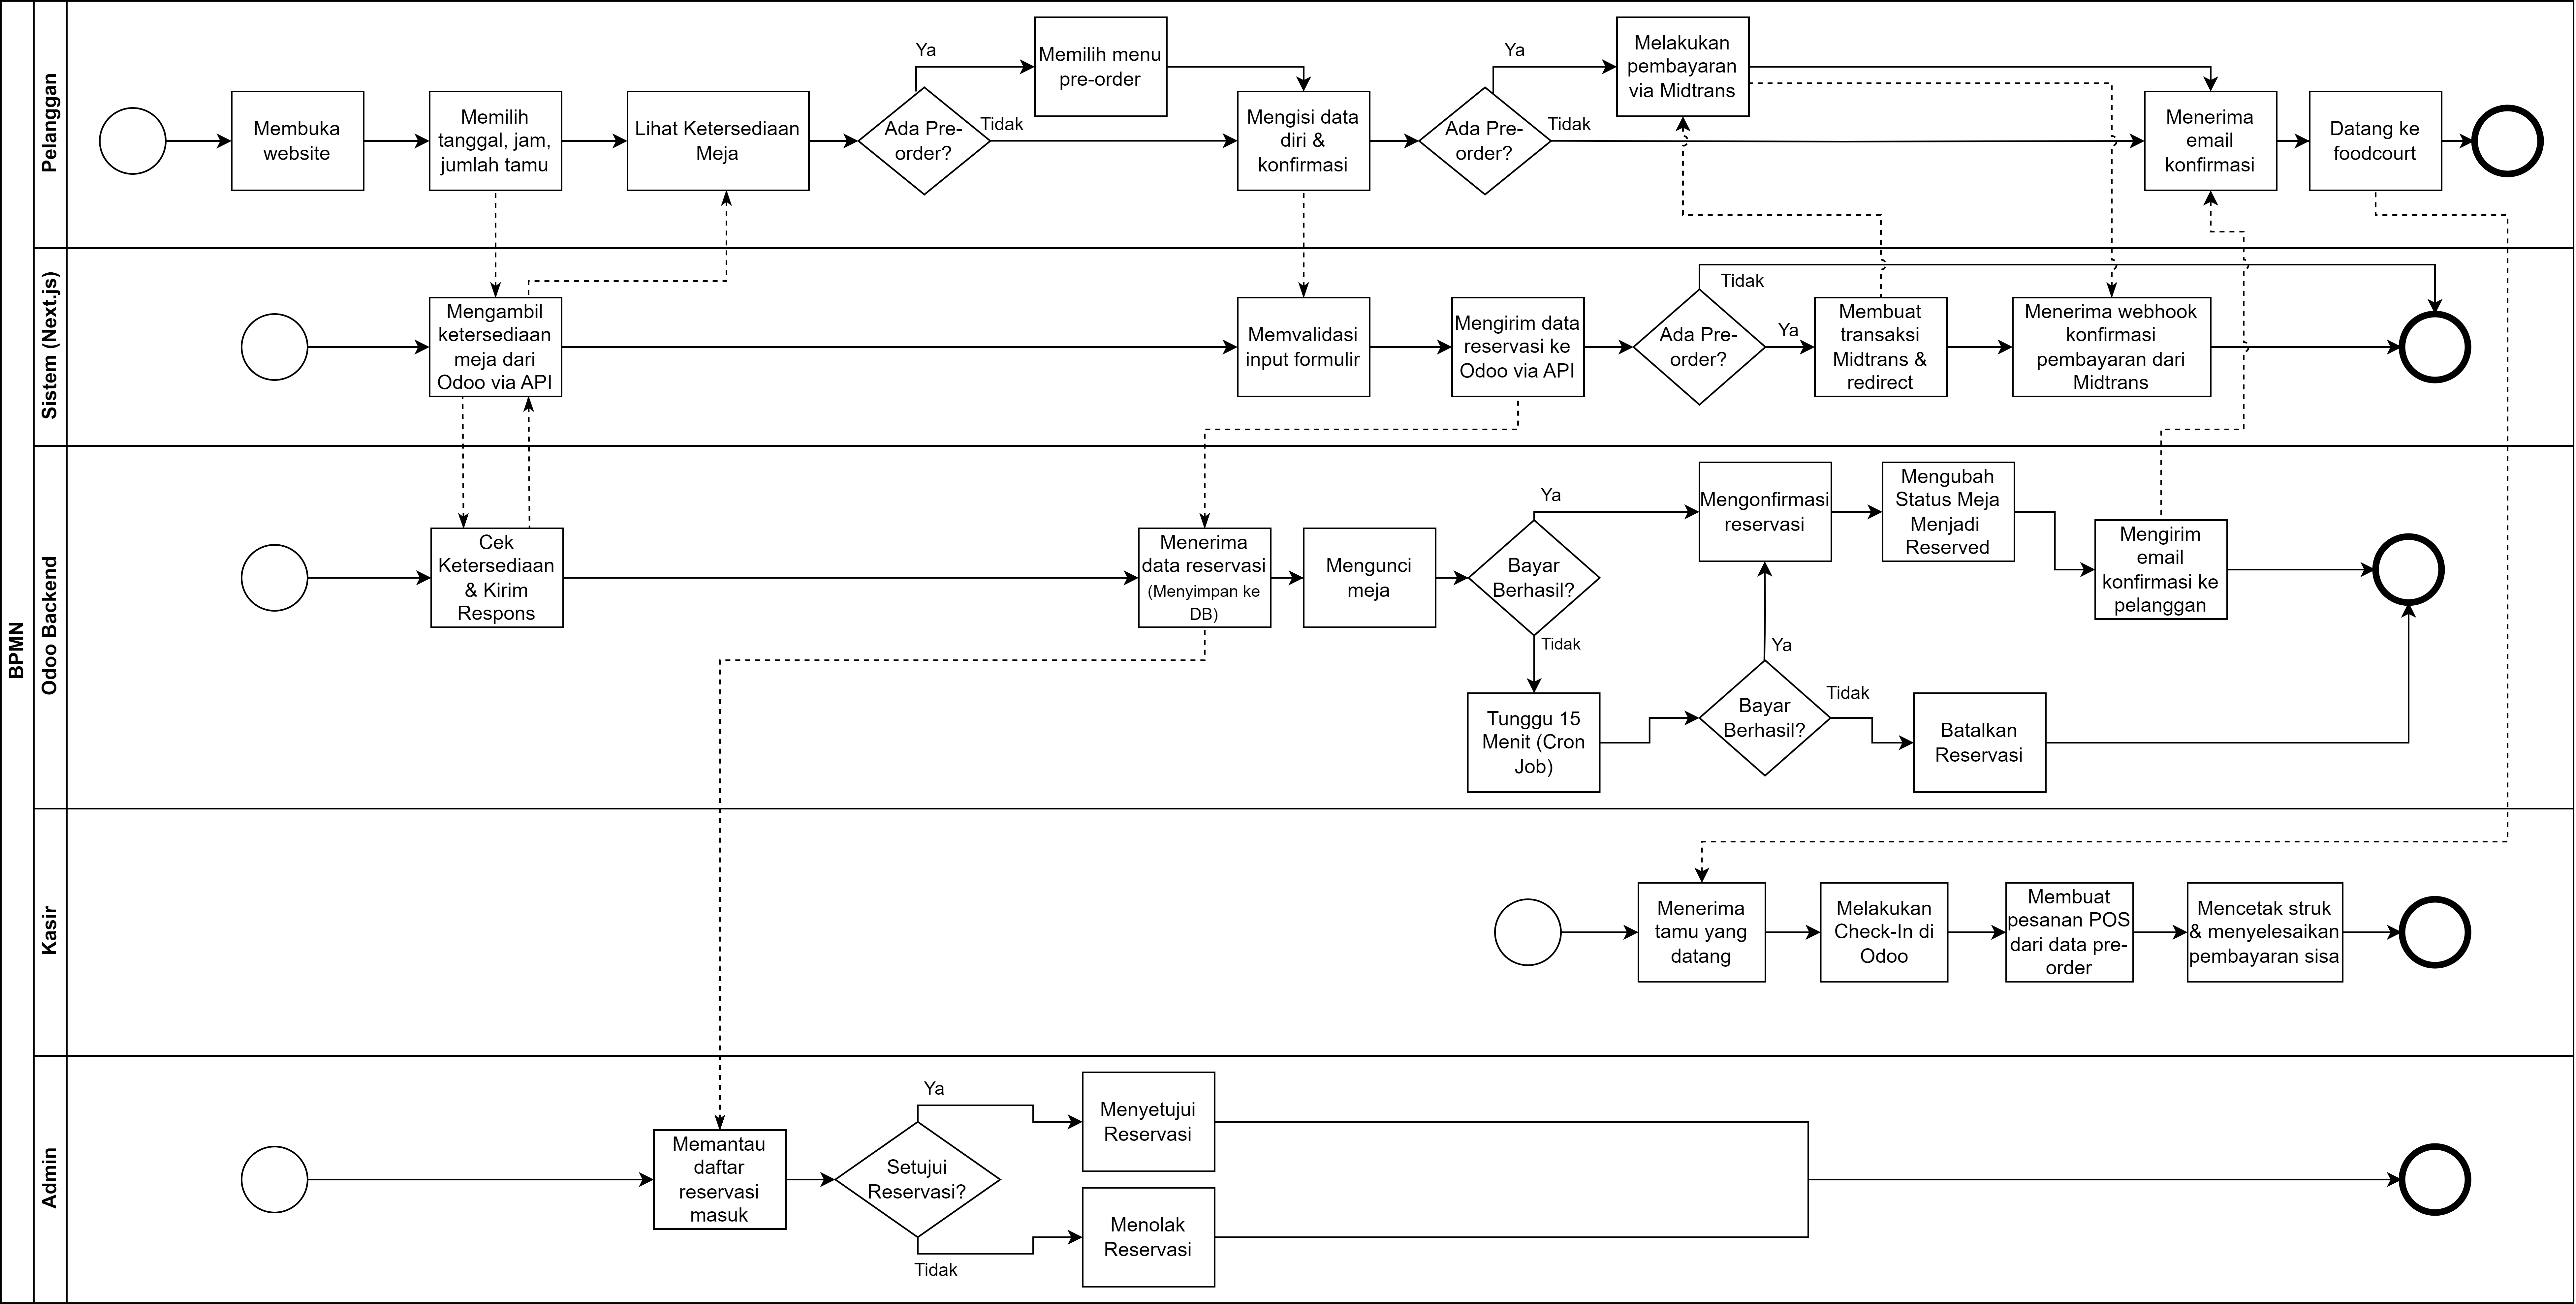
\includegraphics[width=\textwidth]{res/bpmn.png}
    \caption{Diagram BPMN Sistem Reservasi \textit{Food Court}}
    \label{fig:bpmn}
\end{figure*}

\subsection{Use Case Diagram}
\textit{Use Case Diagram} digunakan untuk menunjukkan interaksi dan hak akses masing-masing pengguna di dalam sistem. Karena arsitektur sistem ini dibagi menjadi dua (yaitu \textit{frontend} untuk pelanggan dan \textit{backend} untuk manajemen operasional \textit{food court}), pemodelan \textit{use case} juga dipisahkan sesuai dengan platform masing-masing.

\begin{figure}[htbp]
    \centering
    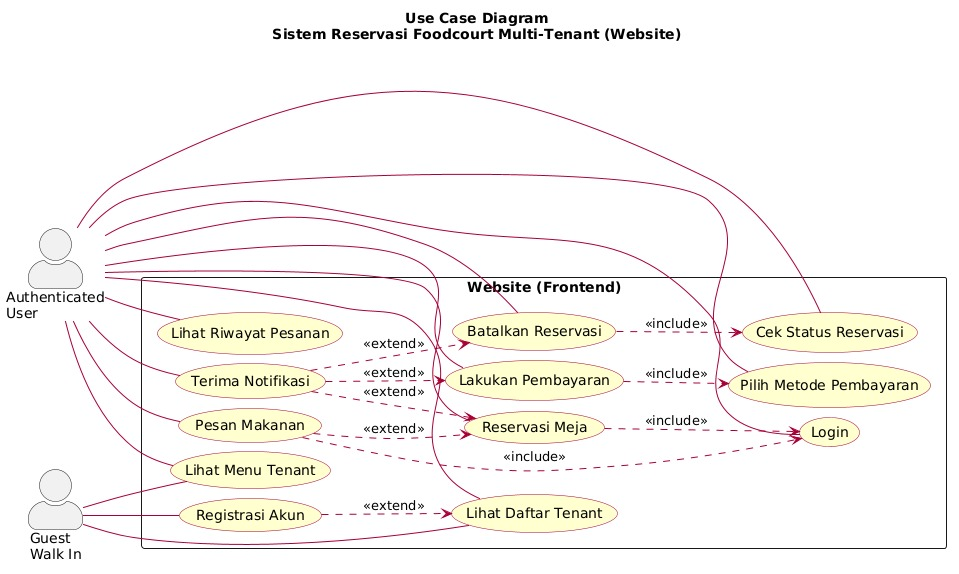
\includegraphics[width=1.0\linewidth]{res/UCD Website.jpeg}
    \caption{Use Case Diagram Sistem Reservasi Foodcourt (Website Frontend)}
    \label{fig:ucd_website}
\end{figure}

Berdasarkan Gambar~\ref{fig:ucd_website}, interaksi pada bagian \textit{Website (Frontend)} melibatkan dua aktor, yaitu \textit{Guest Walk In} dan \textit{Authenticated User}. Aktor \textit{Guest Walk In} memiliki akses terbatas untuk melihat daftar \textit{tenant}, melihat menu \textit{tenant}, serta melakukan registrasi akun. Sementara itu, setelah pelanggan \textit{login} dan menjadi \textit{Authenticated User}, mereka dapat melakukan tindakan yang lebih komprehensif, seperti melakukan reservasi meja, memesan makanan, memilih metode dan melakukan pembayaran, mengecek atau membatalkan status reservasi, menerima notifikasi, hingga melihat riwayat pesanan.

\begin{figure}[htbp]
    \centering
    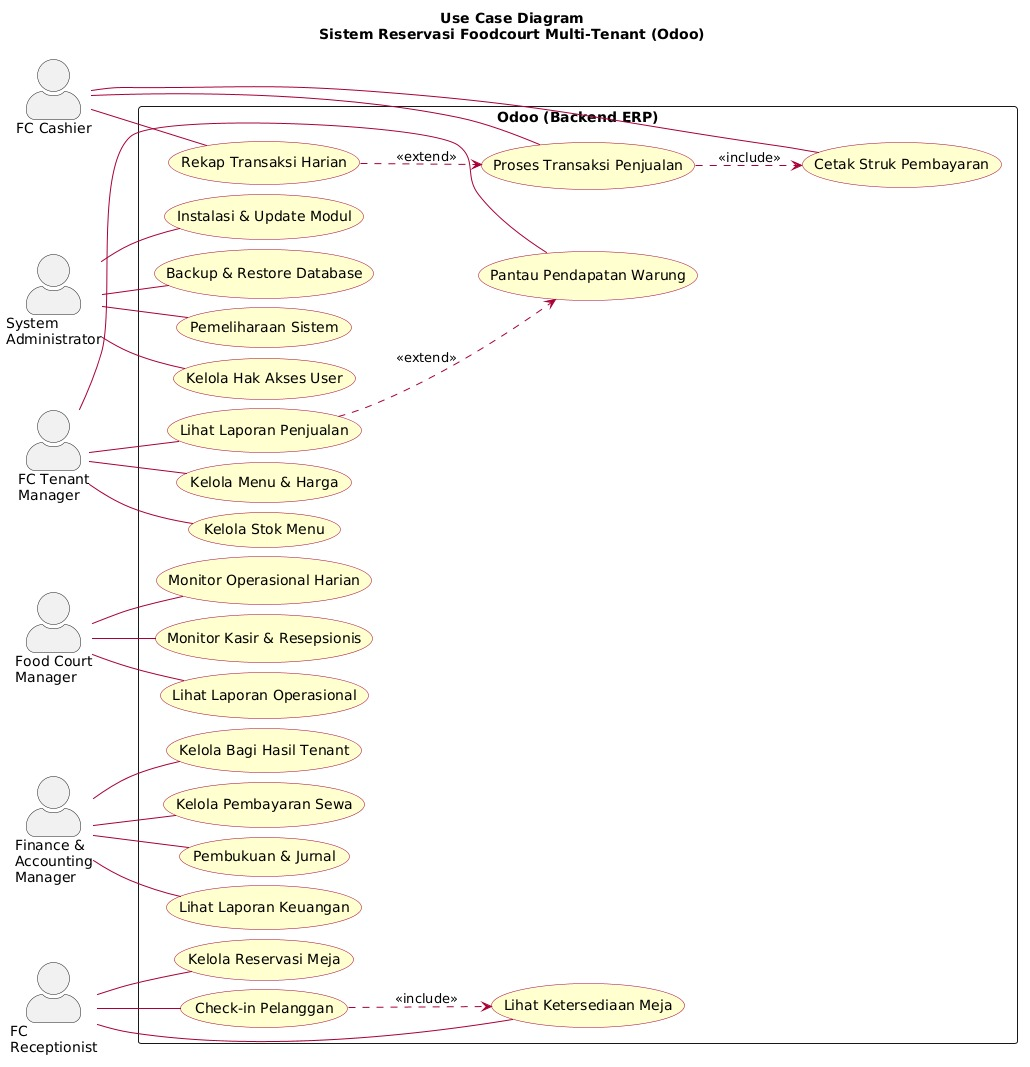
\includegraphics[width=1.0\linewidth]{res/UCD Odoo.jpeg}
    \caption{Use Case Diagram Sistem Reservasi Foodcourt (Odoo Backend ERP)}
    \label{fig:ucd_odoo}
\end{figure}

Di sisi lain, Gambar~\ref{fig:ucd_odoo} mengilustrasikan interaksi pada \textit{Backend ERP (Odoo)} yang berfokus pada manajemen internal \textit{food court}. Terdapat enam aktor dengan peran spesifik sebagai berikut:
\begin{itemize}
    \item \textbf{System Administrator:} Bertanggung jawab atas pengelolaan sistem secara teknis, termasuk mengelola hak akses pengguna, pemeliharaan sistem, \textit{backup \& restore database}, serta instalasi dan pembaruan modul.
    \item \textbf{FC Tenant Manager:} Mengurus operasional masing-masing \textit{tenant}, mulai dari mengelola stok, menu, dan harga, hingga melihat laporan penjualan dan memantau pendapatan warungnya.
    \item \textbf{Food Court Manager:} Bertugas memantau operasional harian secara keseluruhan, memonitor aktivitas kasir dan resepsionis, serta melihat laporan operasional.
    \item \textbf{Finance \& Accounting Manager:} Mengelola aspek keuangan, termasuk pembukuan dan jurnal, kelola pembayaran sewa, perhitungan bagi hasil \textit{tenant}, serta melihat laporan keuangan.
    \item \textbf{FC Cashier:} Berperan dalam memproses transaksi penjualan, mencetak struk pembayaran, dan melakukan rekap transaksi harian.
    \item \textbf{FC Receptionist:} Bertugas melayani pelanggan secara langsung dengan melihat ketersediaan meja, mengelola reservasi meja, dan memproses \textit{check-in} pelanggan.
\end{itemize}

\subsection{Sequence Diagram}
\textit{Sequence Diagram} digunakan untuk menggambarkan interaksi antar objek di dalam dan di sekitar sistem (termasuk Aktor, \textit{Website Frontend}, \textit{Backend Odoo}, dan \textit{Database}) berupa pengiriman pesan terhadap waktu. Berikut adalah \textit{sequence diagram} untuk proses-proses utama pada Sistem Reservasi Foodcourt:

\textbf{1. Registrasi dan Login Pelanggan}
Diagram ini menjelaskan alur pelanggan saat melakukan pendaftaran akun baru dengan mengirimkan data diri, serta proses autentikasi (\textit{login}) dengan memvalidasi kredensial untuk mendapatkan token akses masuk ke dalam sistem.
\begin{figure}[htbp]
    \centering
    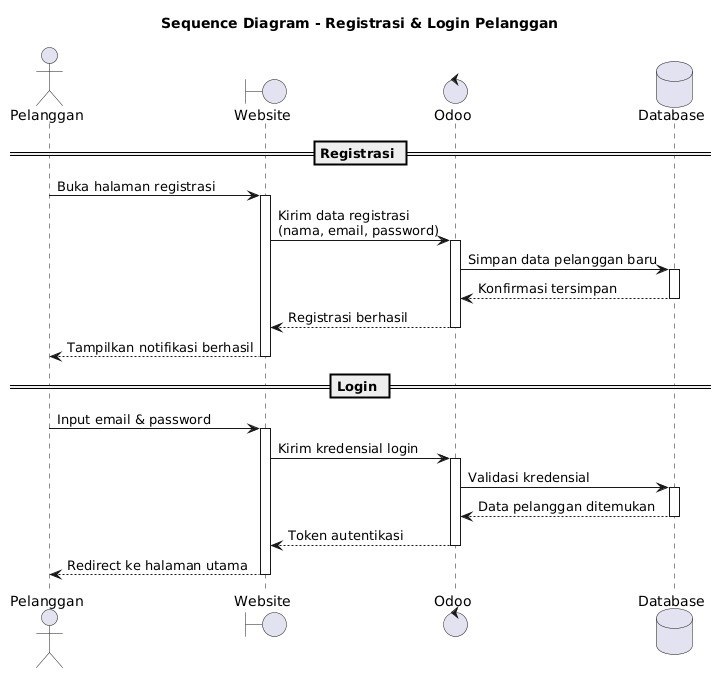
\includegraphics[width=1.0\linewidth]{res/sequence_registrasi dan login.jpeg}
    \caption{Sequence Diagram Registrasi \& Login Pelanggan}
    \label{fig:seq_login}
\end{figure}

\textbf{2. Browse Tenant dan Lihat Menu}
Diagram ini menunjukkan proses penarikan data oleh pelanggan untuk menampilkan daftar \textit{tenant} yang sedang aktif di \textit{food court}, beserta detail katalog menu (nama, harga, gambar, stok) yang ditawarkan oleh \textit{tenant} spesifik.
\begin{figure}[htbp]
    \centering
    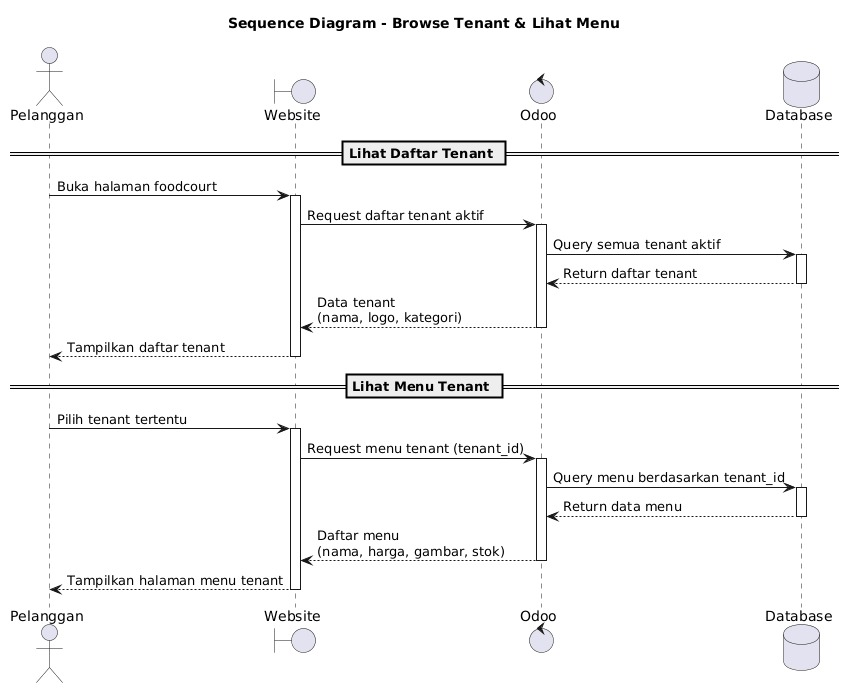
\includegraphics[width=1.0\linewidth]{res/sequence_browse tenant dan lihat menu.jpeg}
    \caption{Sequence Diagram Browse Tenant \& Lihat Menu}
    \label{fig:seq_browse}
\end{figure}

\textbf{3. Reservasi Meja Foodcourt}
Diagram ini menggambarkan tahapan pelanggan dalam mencari ketersediaan meja berdasarkan parameter tanggal, waktu, dan kapasitas orang. Setelah meja dipilih, sistem akan memproses pesanan tersebut ke \textit{database} dan mengembalikan kode \textit{booking} kepada pelanggan.
\begin{figure}[htbp]
    \centering
    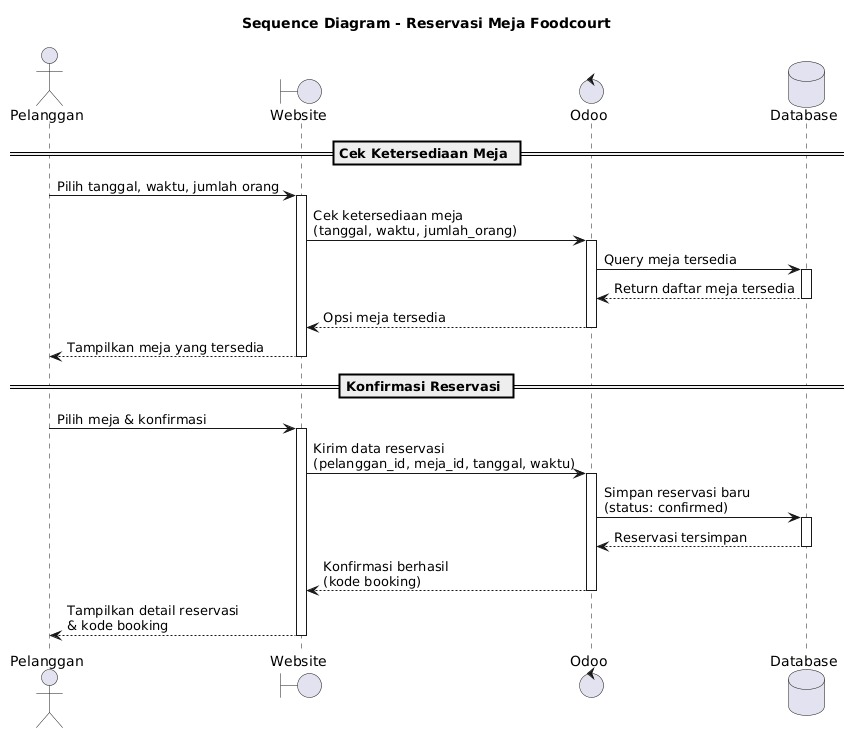
\includegraphics[width=1.0\linewidth]{res/sequence_reservasi meja foodcourt.jpeg}
    \caption{Sequence Diagram Reservasi Meja Foodcourt}
    \label{fig:seq_reservasi}
\end{figure}

\textbf{4. Pemesanan Makanan}
Diagram ini menjelaskan alur pelanggan ketika menambahkan makanan ke keranjang hingga melakukan proses \textit{checkout}. Terdapat pengecekan kondisi (\textit{alt frame}) oleh sistem Odoo untuk memvalidasi ketersediaan stok; order akan disimpan jika stok tersedia, atau sistem akan menampilkan pesan penolakan jika stok habis.
\begin{figure}[htbp]
    \centering
    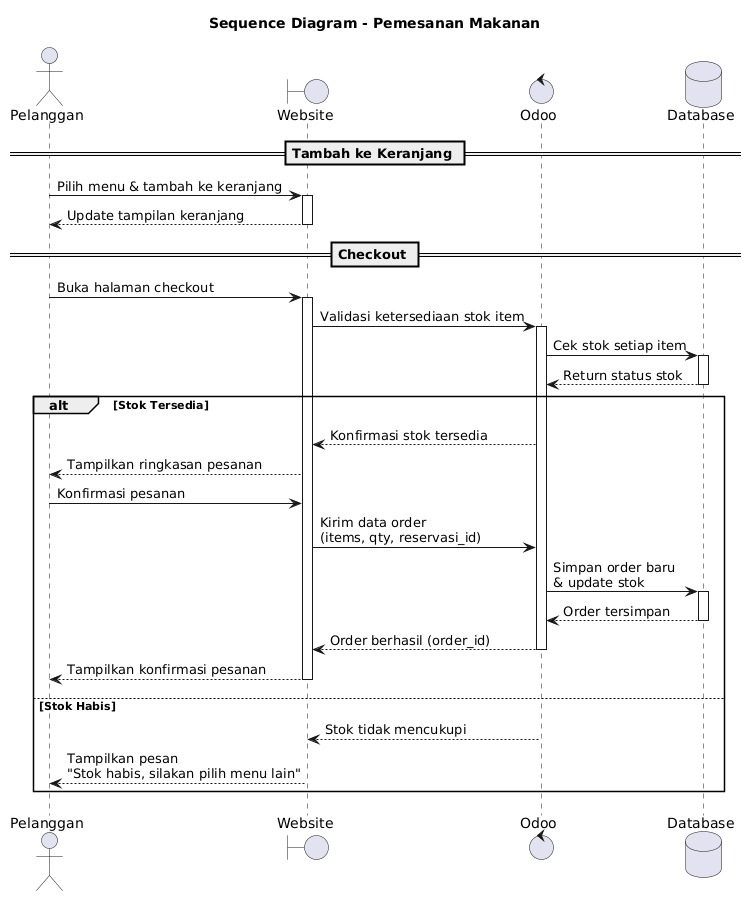
\includegraphics[width=1.0\linewidth]{res/sequence_pemesanan makanan.jpeg}
    \caption{Sequence Diagram Pemesanan Makanan}
    \label{fig:seq_pesan_makanan}
\end{figure}

\textbf{5. Cek Status Reservasi}
Diagram ini mengilustrasikan proses penarikan data riwayat reservasi milik pelanggan. Pelanggan juga dapat memilih salah satu riwayat untuk me-\textit{request} detail lengkap dari reservasi tersebut beserta pesanan (\textit{order}) yang terkait di dalamnya.
\begin{figure}[htbp]
    \centering
    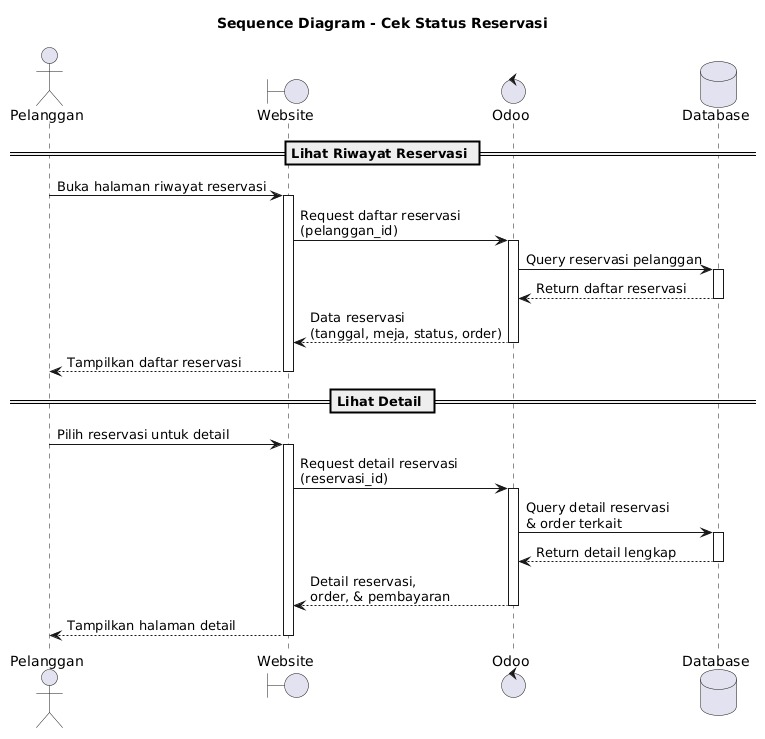
\includegraphics[width=1.0\linewidth]{res/sequence_cek status reservasi.jpeg}
    \caption{Sequence Diagram Cek Status Reservasi}
    \label{fig:seq_cek_status}
\end{figure}

\textbf{6. Pembatalan Reservasi}
Diagram ini menampilkan skenario ketika pelanggan mengajukan pembatalan reservasi. Sistem akan memvalidasi kebijakan batas waktu pembatalan melalui blok alternatif (\textit{alt}). Jika disetujui, status reservasi dibatalkan dan meja kembali tersedia; jika melewati batas waktu, permintaan pembatalan akan ditolak.
\begin{figure}[htbp]
    \centering
    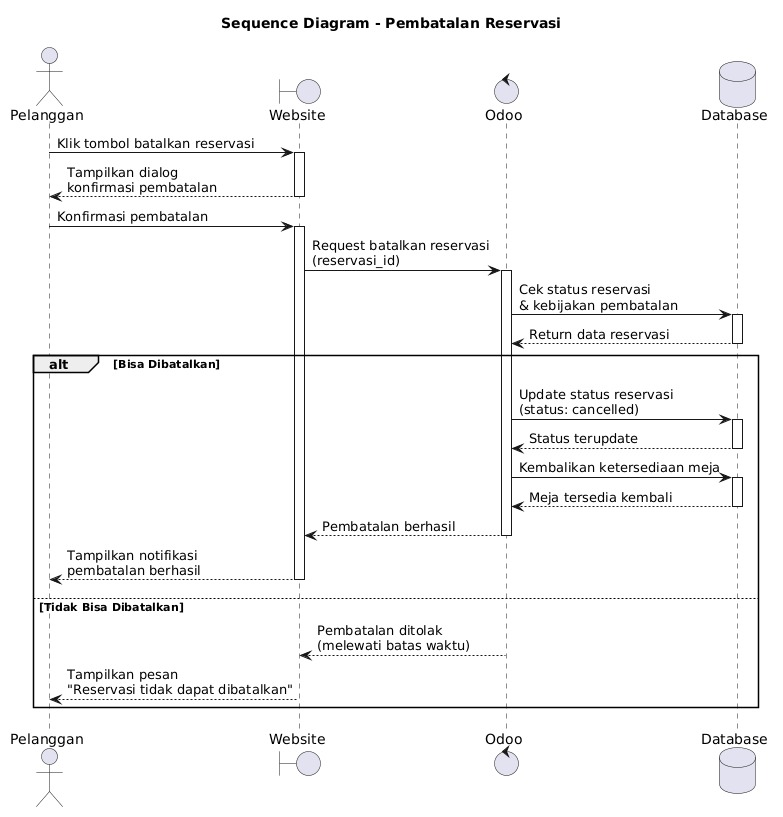
\includegraphics[width=1.0\linewidth]{res/sequence_pembatalan reservasi.jpeg}
    \caption{Sequence Diagram Pembatalan Reservasi}
    \label{fig:seq_batal_reservasi}
\end{figure}

\subsection{Kebutuhan Sistem}
Kebutuhan fungsional pada sistem ini dibagi menjadi dua bagian agar sesuai dengan pembagian arsitektur \textit{frontend} dan \textit{backend}.

\subsubsection{Kebutuhan Fungsional Web Frontend (Next.js)}
\textit{Web Frontend} berfungsi sebagai antarmuka utama bagi pelanggan. Fitur-fitur yang harus dipenuhi pada bagian ini antara lain:
\begin{itemize}
    \item \textbf{Registrasi dan Autentikasi:} Sistem memungkinkan pelanggan untuk mendaftar akun baru dan \textit{login}. Data akun disimpan di \textit{database} lokal Next.js dan diintegrasikan dengan data kontak di Odoo.
    \item \textbf{Pencarian Meja Kosong:} Sistem harus bisa menampilkan daftar meja yang tersedia berdasarkan tanggal, jam, dan area. Data ini diambil langsung secara \textit{real-time} melalui API Odoo.
    \item \textbf{Pembuatan Reservasi:} Sistem menyediakan \textit{form} reservasi meja, baik bagi pengguna yang sudah \textit{login} maupun pengguna tamu (\textit{guest}). Data reservasi ini selanjutnya dikirim ke Odoo.
    \item \textbf{Riwayat Reservasi:} Sistem dapat mengambil data dari Odoo untuk menampilkan daftar reservasi yang pernah dilakukan oleh pelanggan.
\end{itemize}

\subsubsection{Kebutuhan Fungsional Backend (Odoo ERP)}
Backend yang menggunakan Odoo berfungsi sebagai pusat data dan logika bisnis khusus untuk admin dan tenant. Fitur-fitur utamanya meliputi:
\begin{itemize}
    \item \textbf{Kelola Reservasi:} Admin dapat melihat daftar pesanan, serta menerima, menolak, atau membatalkan reservasi. Hal ini termasuk fitur melepas kunci (\textit{lock}) meja jika reservasi batal.
    \item \textbf{Penyediaan API (XML-RPC):} Sistem harus menyediakan API agar \textit{Web Frontend} dapat mengambil dan menyimpan data tanpa menyebabkan bentrok pada jadwal meja.
    \item \textbf{Manajemen Master Data:} Admin memiliki akses untuk menginput atau mengubah master data, seperti data meja (kapasitas dan lokasinya), serta daftar tenant.
    \item \textbf{Point of Sale (POS):} Sistem harus memiliki antarmuka kasir (POS) untuk memproses pesanan dan pembayaran untuk setiap tenant.
    \item \textbf{Dasbor Analitik dan Pelaporan:} Sistem harus mampu mengolah data transaksi dan operasional secara otomatis untuk disajikan dalam bentuk grafik visual. Hal ini memungkinkan admin untuk memantau metrik kunci seperti tingkat okupansi meja, waktu tersibuk, dan performa penjualan masing-masing tenant secara \textit{real-time}.
\end{itemize}

\section{PERANCANGAN SISTEM}

\subsection{Arsitektur Sistem Terintegrasi}
Sistem Reservasi \textit{Food Court} ini dirancang menggunakan arsitektur yang terpisah (\textit{decoupled architecture}), di mana antarmuka pengguna (\textit{Web Frontend}) dan sistem pengelolaan data (\textit{Backend}) berdiri sendiri namun terhubung melalui API. Pendekatan ini dipilih untuk memberikan pengalaman pengguna yang cepat dan responsif di sisi pelanggan, sembari menjaga keandalan pengelolaan operasional di sisi manajemen.

Arsitektur ini terdiri dari dua komponen utama. Pertama, \textit{Web Frontend} dibangun menggunakan \textit{framework} Next.js. Komponen ini melayani interaksi langsung dengan pelanggan, seperti pencarian meja dan pengisian form reservasi. Kedua, \textit{Backend} dibangun menggunakan Odoo ERP. Komponen ini bertindak sebagai pusat basis data, logika bisnis, dan antarmuka bagi admin serta tenant. Komunikasi antara kedua sistem ini dijembatani menggunakan XML-RPC API bawaan Odoo, yang memungkinkan Next.js untuk melakukan validasi ketersediaan meja dan mengirimkan data reservasi baru secara \textit{real-time} tanpa mengekspos basis data Odoo secara langsung ke publik.

\begin{figure}[htbp]
    \centering
    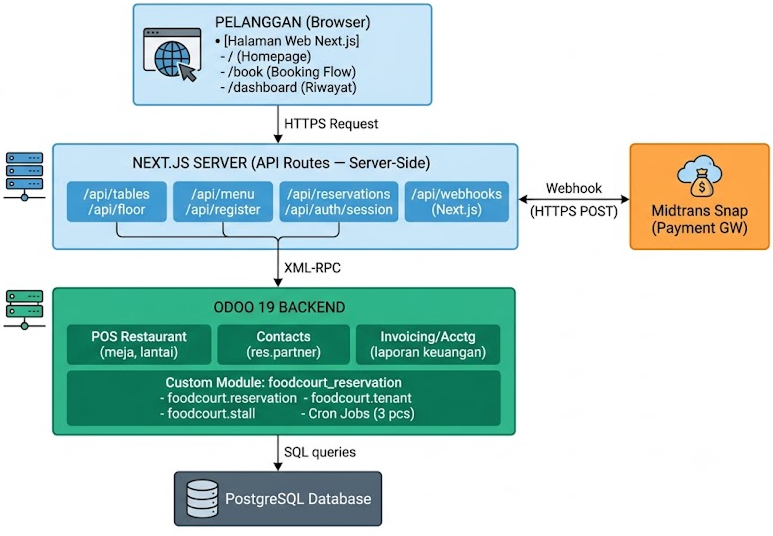
\includegraphics[width=1.0\linewidth]{res/architecture.png}
    \caption{Arsitektur Sistem Next.js dan Odoo}
    \label{fig:architecture}
\end{figure}

\subsection{Perancangan Modul Odoo (Backend)}
Untuk membangun fondasi \textit{backend} yang tangguh, sistem ini memanfaatkan beberapa modul dasar bawaan Odoo yang dikombinasikan dengan modul kustom. Modul-modul dasar tersebut meliputi:
\begin{itemize}
    \item \textbf{Modul Point of Sale (POS) Restaurant:} Merupakan modul inti yang digunakan untuk mengelola denah lantai (\textit{floor plan}) dan daftar meja. Modul ini juga digunakan oleh tenant dan kasir untuk memproses pesanan serta pembayaran pelanggan secara langsung.
    \item \textbf{Modul Contacts:} Digunakan untuk menyimpan dan mengelola data profil pelanggan. Setiap kali pelanggan baru mendaftar melalui \textit{web}, sistem akan secara otomatis membuatkan entitas \textit{Contact} (Partner) baru di dalam Odoo sehingga data terpusat.
    \item \textbf{Modul Invoicing / Accounting:} Modul ini terintegrasi langsung dengan POS untuk mencatat seluruh arus kas masuk, mengelola pajak, dan menerbitkan laporan pendapatan operasional harian.
\end{itemize}

Selain menggabungkan modul bawaan tersebut, dikembangkan pula modul kustom (\textit{custom addons}) bernama \texttt{foodcourt\_reservation}. Modul ini dirancang secara khusus untuk menangani fitur yang tidak ada di versi bawaan, seperti sistem pemesanan (reservasi) meja di muka, logika penguncian meja (\textit{lock system}), serta menyediakan \textit{endpoint} API khusus agar Next.js dapat menarik data ketersediaan meja dengan lebih mudah. Fitur \textbf{Analitik dan Pelaporan} juga disatukan ke dalam modul kustom ini, sehingga data operasional dari reservasi dan POS langsung diolah untuk kebutuhan evaluasi manajemen secara otomatis.

\subsection{Perancangan Basis Data (ERD)}
Perancangan basis data memegang peran penting dalam memastikan konsistensi data antara operasional harian dan riwayat reservasi. Basis data utama seluruhnya dikelola oleh PostgreSQL yang berada di bawah ekosistem Odoo.

\begin{figure}[htbp]
    \centering
    \includegraphics[width=1.0\linewidth]{res/erd.png}
    \caption{Entity Relationship Diagram (ERD)}
    \label{fig:erd}
\end{figure}

Struktur basis data modul kustom reservasi ini tidak berdiri sendiri, melainkan terhubung dan mewarisi data dari modul-modul inti Odoo lainnya guna menjaga konsistensi ekosistem ERP. Relasi utamanya meliputi:
\begin{itemize}
    \item \textbf{Relasi ke Modul Contacts (\texttt{res.partner}):} Data pelanggan dan data pemilik tenant dihubungkan secara terpusat ke tabel ini. Tabel reservasi (\texttt{foodcourt.reservation}) menggunakan \textit{Foreign Key} \texttt{customer\_id} yang merujuk ke tabel ini untuk mencatat identitas pemesan.
    \item \textbf{Relasi ke Modul POS Restaurant (\texttt{restaurant.table} \& \texttt{restaurant.floor}):} Tabel reservasi secara langsung berelasi dengan tabel meja bawaan POS Odoo. Hal ini memastikan bahwa status ketersediaan (\textit{lock mechanism}) diterapkan pada aset meja yang sebenarnya dikelola oleh sistem POS, bukan pada tabel bayangan.
    \item \textbf{Relasi ke Modul POS (\texttt{pos.order}):} Setelah pelanggan melakukan pemesanan menu, sistem akan menautkan ID reservasi tersebut ke dalam tabel pesanan POS. Ini memungkinkan struk pembayaran secara akurat mencantumkan nama pelanggan dan meja yang telah direservasi sebelumnya.
    \item \textbf{Relasi ke Modul Inventory (\texttt{product.template}):} Setiap menu makanan yang ditambahkan oleh tenant berelasi langsung dengan master data produk Odoo, di mana modul kustom menambahkan \textit{field} khusus agar sistem mengenali menu milik tenant mana.
\end{itemize}

Desain relasional yang mengandalkan keterhubungan antar-modul ini memastikan bahwa tidak ada duplikasi data, serta memudahkan integrasi data lintas departemen, mulai dari operasional lapangan hingga laporan keuangan.

\subsection{Perancangan Endpoint API}
Untuk menghubungkan \textit{Web Frontend} Next.js dengan \textit{Backend} Odoo, sistem memanfaatkan jembatan komunikasi berupa XML-RPC API bawaan Odoo. Pendekatan ini memungkinkan kedua sistem untuk bertukar data secara mulus, sehingga setiap perubahan di Odoo akan langsung tercermin di \textit{website}, dan sebaliknya. 

Beberapa \textit{endpoint} atau fungsi API utama yang dirancang untuk kebutuhan integrasi ini meliputi:
\begin{itemize}
    \item \textbf{Pencarian Ketersediaan Meja:} Next.js akan mengirimkan parameter pencarian (tanggal, jam, dan lantai) menggunakan metode pemanggilan API ke Odoo. Odoo kemudian memproses logika ketersediaan dan mengembalikan daftar meja yang statusnya tersedia dan tidak bentrok dengan jadwal lain.
    \item \textbf{Pembuatan Kontak Pelanggan:} Saat pelanggan mendaftar akun di \textit{web}, Next.js akan memanggil metode pembuatan data (\textit{create}) ke model \texttt{res.partner} di Odoo untuk membuatkan profil kontak baru secara terpusat.
    \item \textbf{Submit Reservasi:} Setelah pelanggan mengisi formulir, Next.js mengirimkan sekumpulan data menuju model \texttt{foodcourt.reservation}. Sistem Odoo kemudian akan mengunci slot waktu tersebut secara otomatis.
    \item \textbf{Riwayat Transaksi:} Untuk memuat halaman profil, Next.js akan menarik seluruh data reservasi yang terhubung dengan ID pelanggan yang sedang masuk (\textit{login}) agar dapat ditampilkan sebagai riwayat.
\end{itemize}

\subsection{Perancangan Antarmuka (UI/UX)}
Antarmuka pelanggan pada aplikasi \textit{Web Frontend} dirancang dengan mengutamakan kemudahan penggunaan (\textit{user-friendly}) dan responsivitas, sehingga nyaman diakses baik dari ponsel pintar maupun komputer. Desain antarmuka difokuskan pada halaman-halaman esensial, antara lain:

\subsubsection{Halaman Utama (\textit{Homepage})}
Menampilkan informasi ringkas mengenai \textit{food court} dan tombol panggil tindakan (\textit{call to action}) untuk mulai mencari meja.
\begin{figure}[htbp]
    \centering
    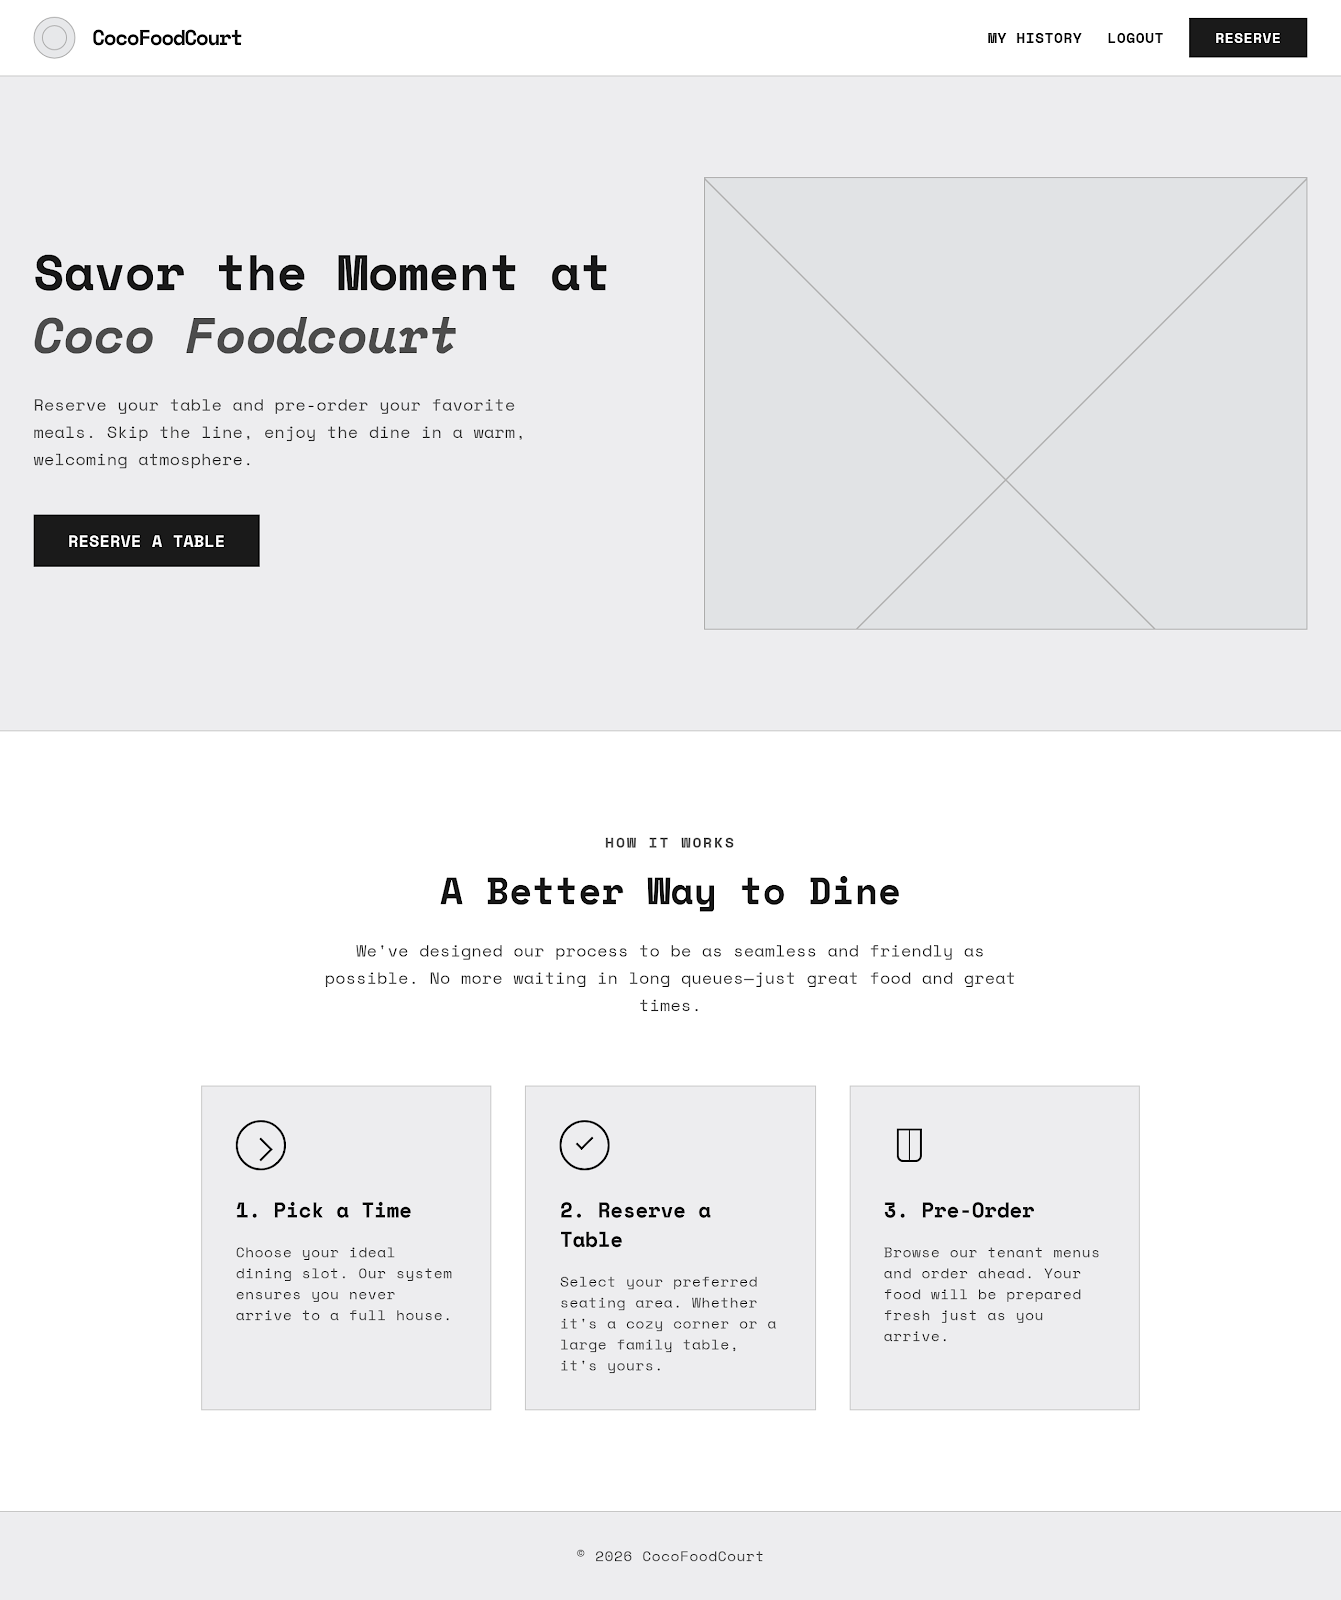
\includegraphics[width=1.0\linewidth]{res/ui_homepage_placeholder.png}
    \caption{Rancangan Antarmuka Halaman Utama}
    \label{fig:ui_homepage}
\end{figure}

\subsubsection{Halaman Alur Reservasi (\textit{Multi-step Booking})}
Halaman ini merupakan inti dari interaksi pelanggan, yang dirancang menggunakan alur bertahap (\textit{multi-step form}) untuk memandu pelanggan secara intuitif tanpa membebani mereka dengan terlalu banyak informasi dalam satu layar. Alur ini dibagi menjadi empat tahap dengan antarmuka masing-masing:

\textbf{Tahap 1 - Waktu \& Jumlah Tamu:}
Pada tahap pertama, pelanggan memasukkan preferensi tanggal, jam kedatangan, serta jumlah tamu yang akan hadir.
\begin{figure}[htbp]
    \centering
    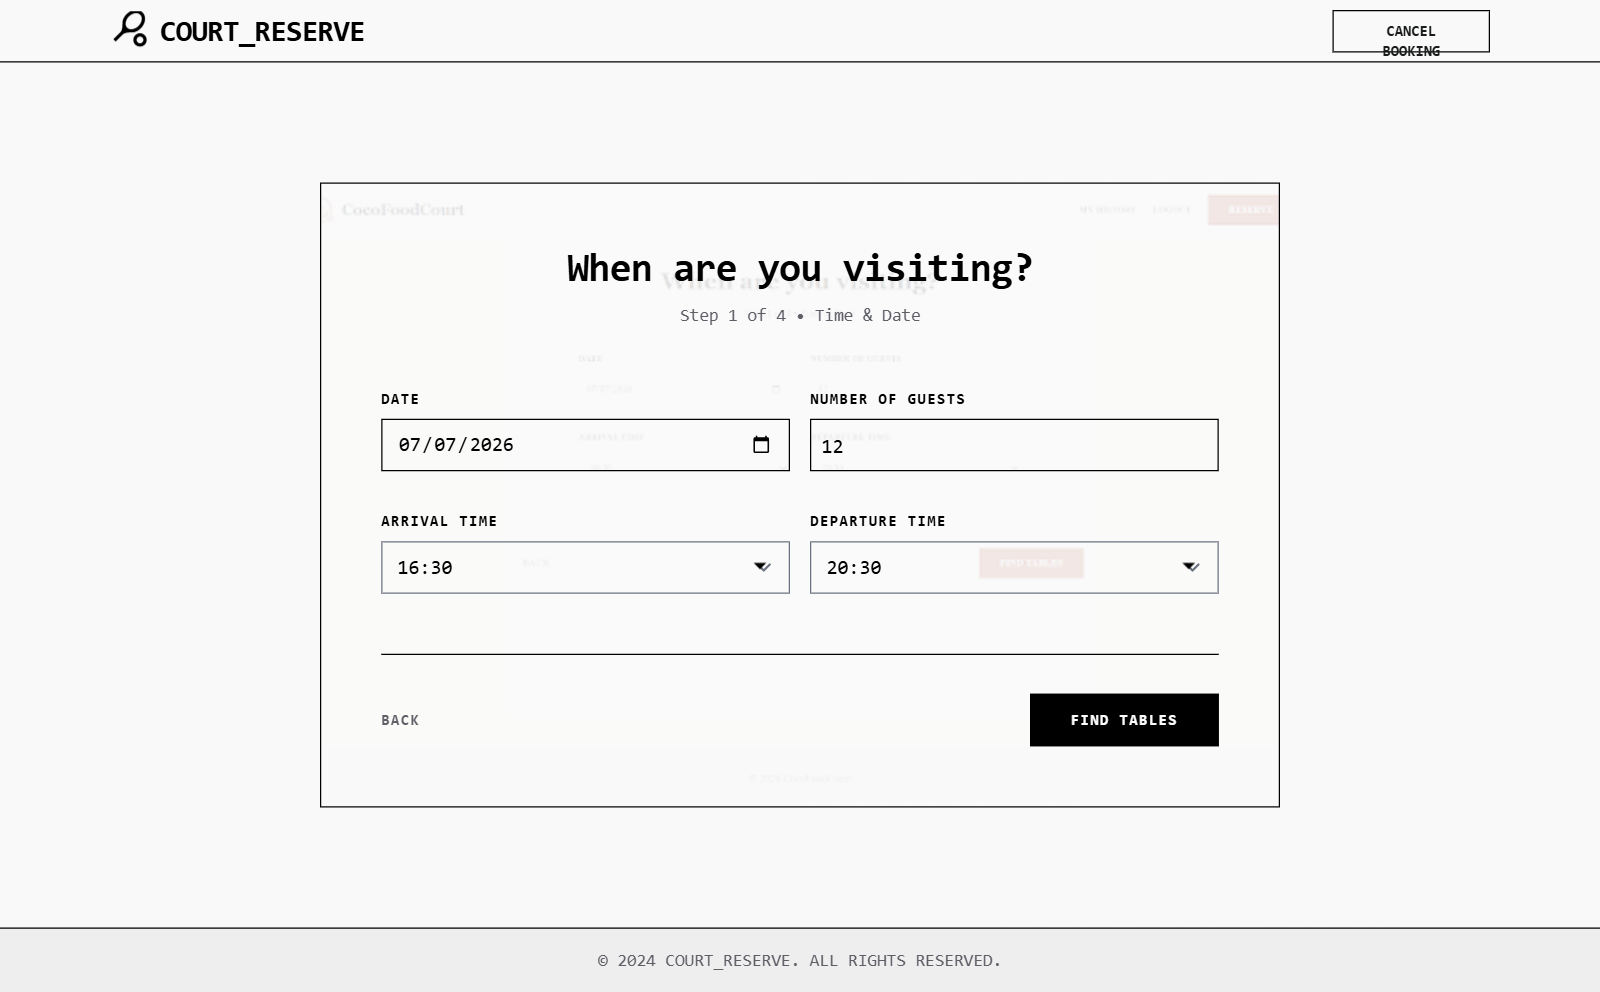
\includegraphics[width=1.0\linewidth]{res/ui_booking_step1_placeholder.png}
    \caption{Rancangan Antarmuka - Tahap 1 Waktu \& Tamu}
    \label{fig:ui_step1}
\end{figure}

\textbf{Tahap 2 - Pemilihan Meja:}
Setelah memasukkan waktu, sistem menampilkan denah atau daftar meja yang berstatus "Tersedia" sesuai dengan parameter yang diberikan.
\begin{figure}[htbp]
    \centering
    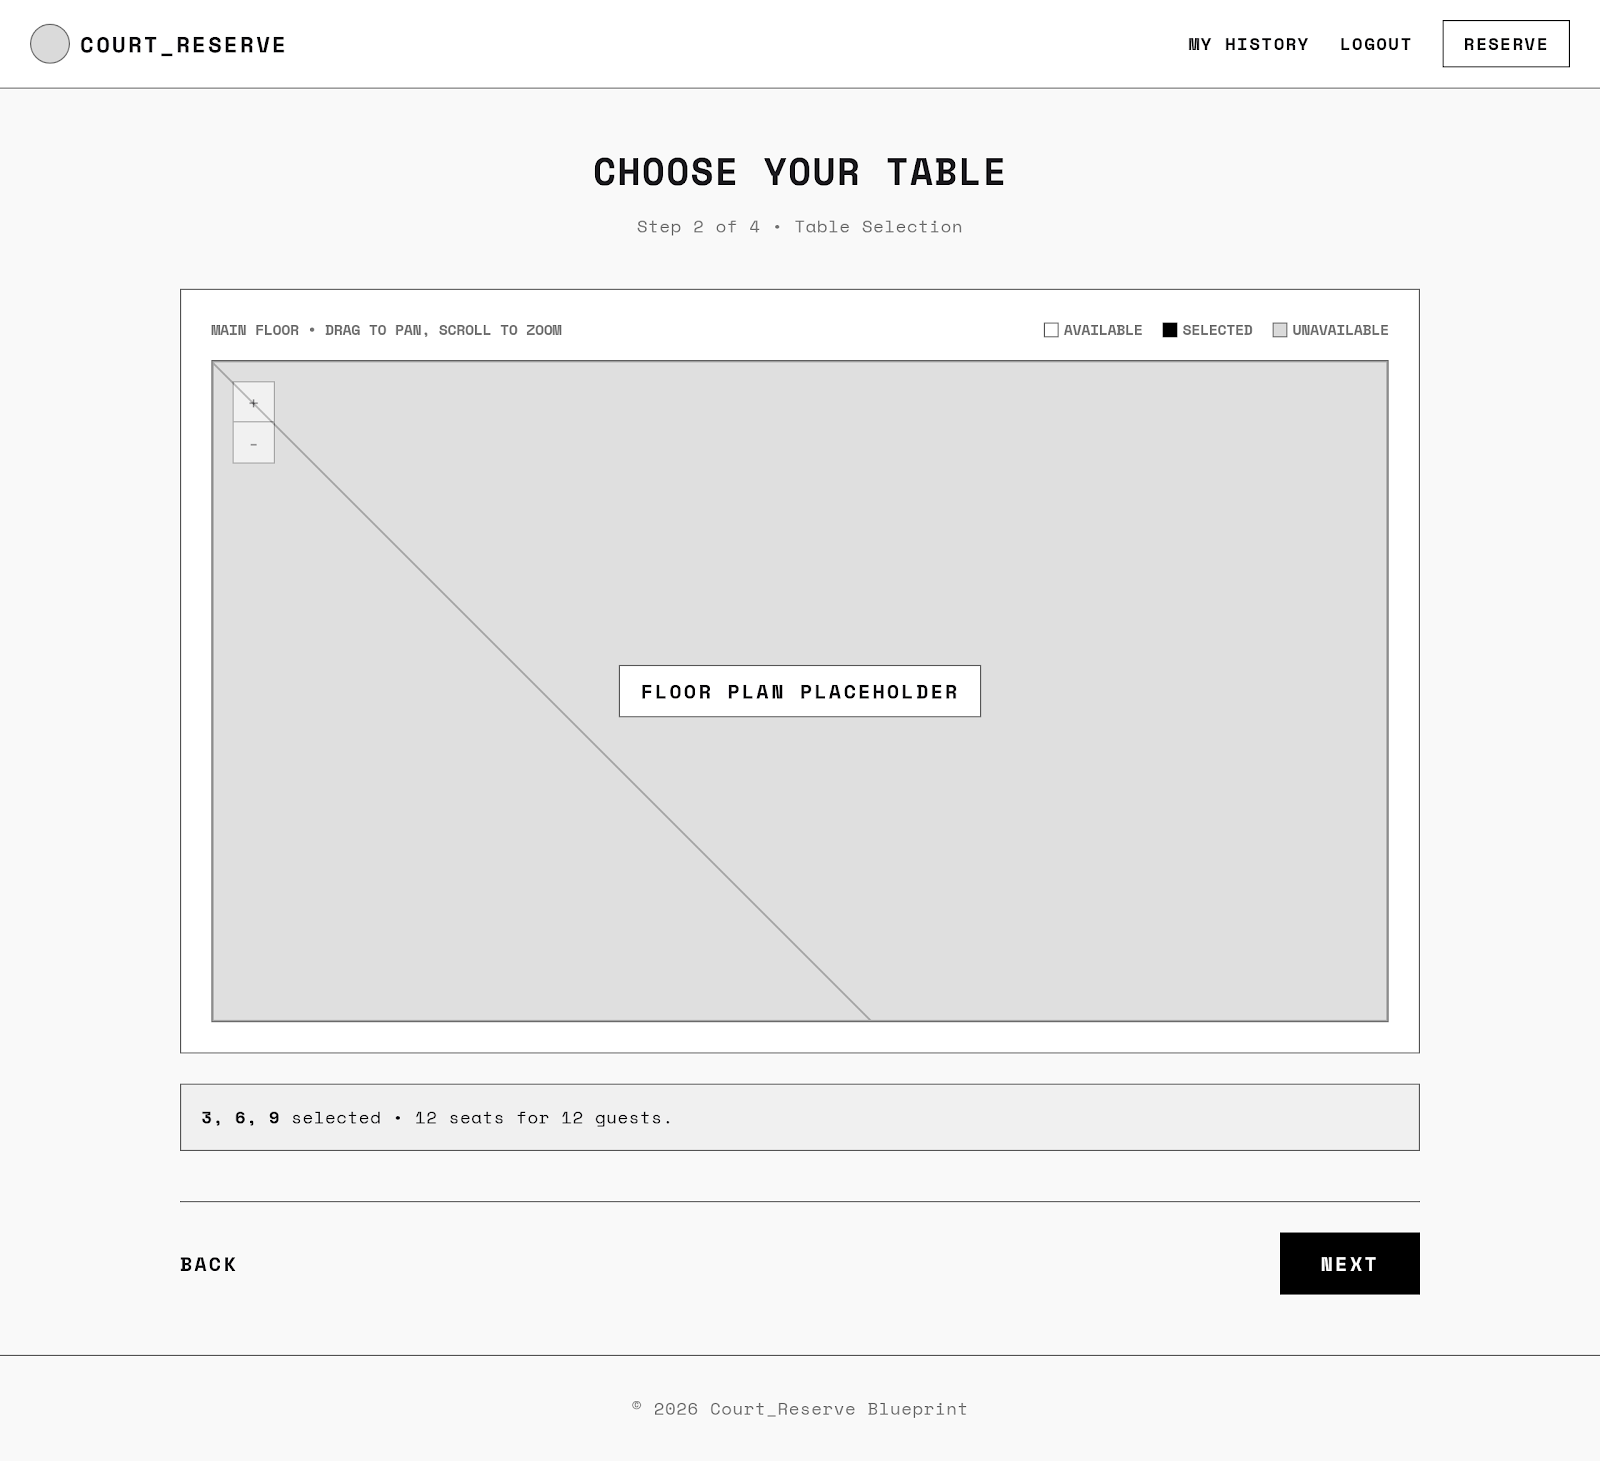
\includegraphics[width=1.0\linewidth]{res/ui_booking_step2_placeholder.png}
    \caption{Rancangan Antarmuka - Tahap 2 Pemilihan Meja}
    \label{fig:ui_step2}
\end{figure}

\textbf{Tahap 3 - Pemilihan Menu Makanan:}
Pelanggan kemudian diarahkan untuk memilih makanan dan minuman dari berbagai tenant yang tersedia untuk dipesan secara \textit{pre-order}.
\begin{figure}[htbp]
    \centering
    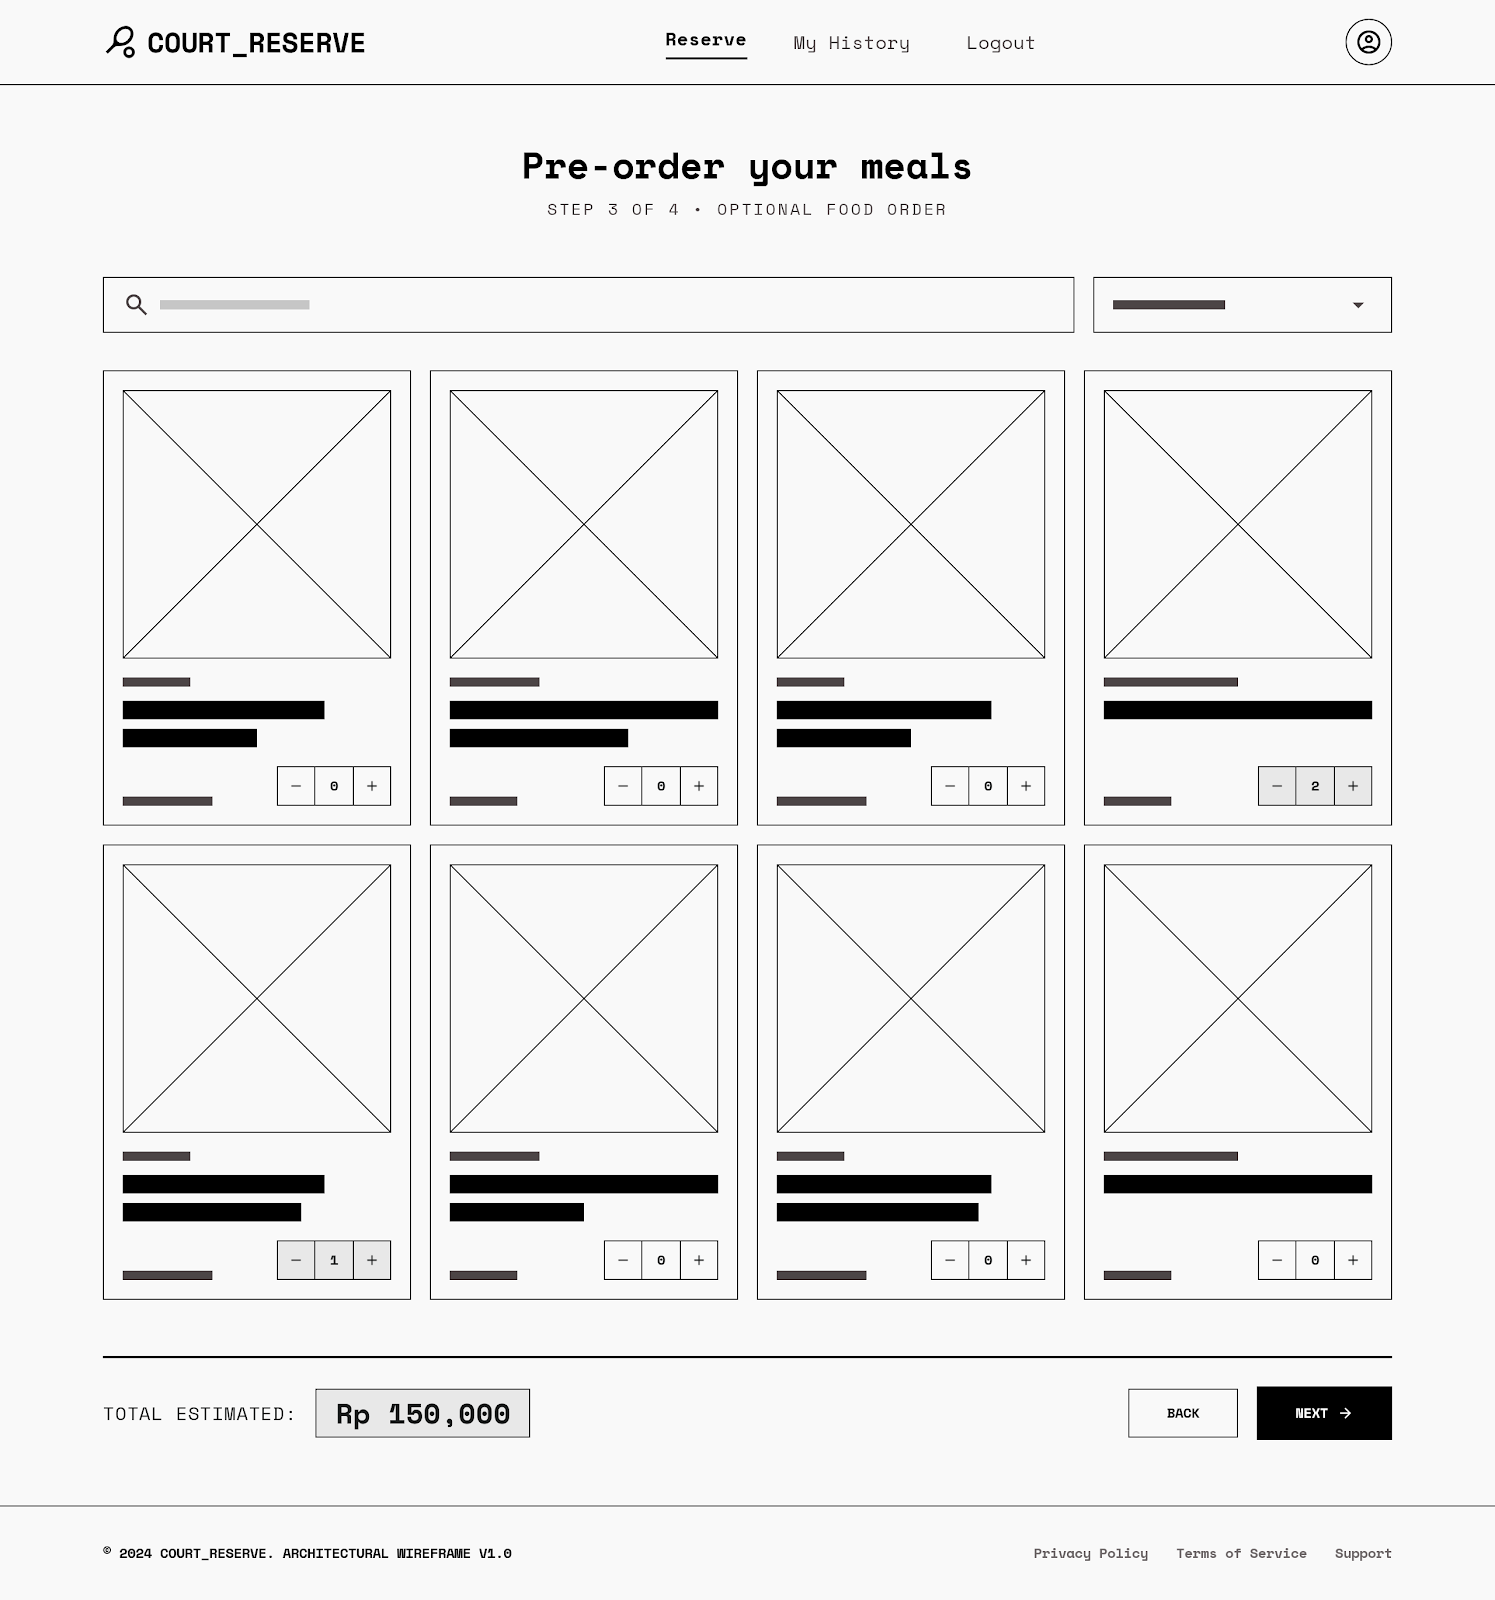
\includegraphics[width=1.0\linewidth]{res/ui_booking_step3_placeholder.png}
    \caption{Rancangan Antarmuka - Tahap 3 Pemilihan Menu}
    \label{fig:ui_step3}
\end{figure}

\textbf{Tahap 4 - Finalisasi:}
Tahap terakhir berupa halaman ringkasan yang menampilkan data pelanggan, detail reservasi, total tagihan, serta instruksi konfirmasi (\textit{Checkout}).
\begin{figure}[htbp]
    \centering
    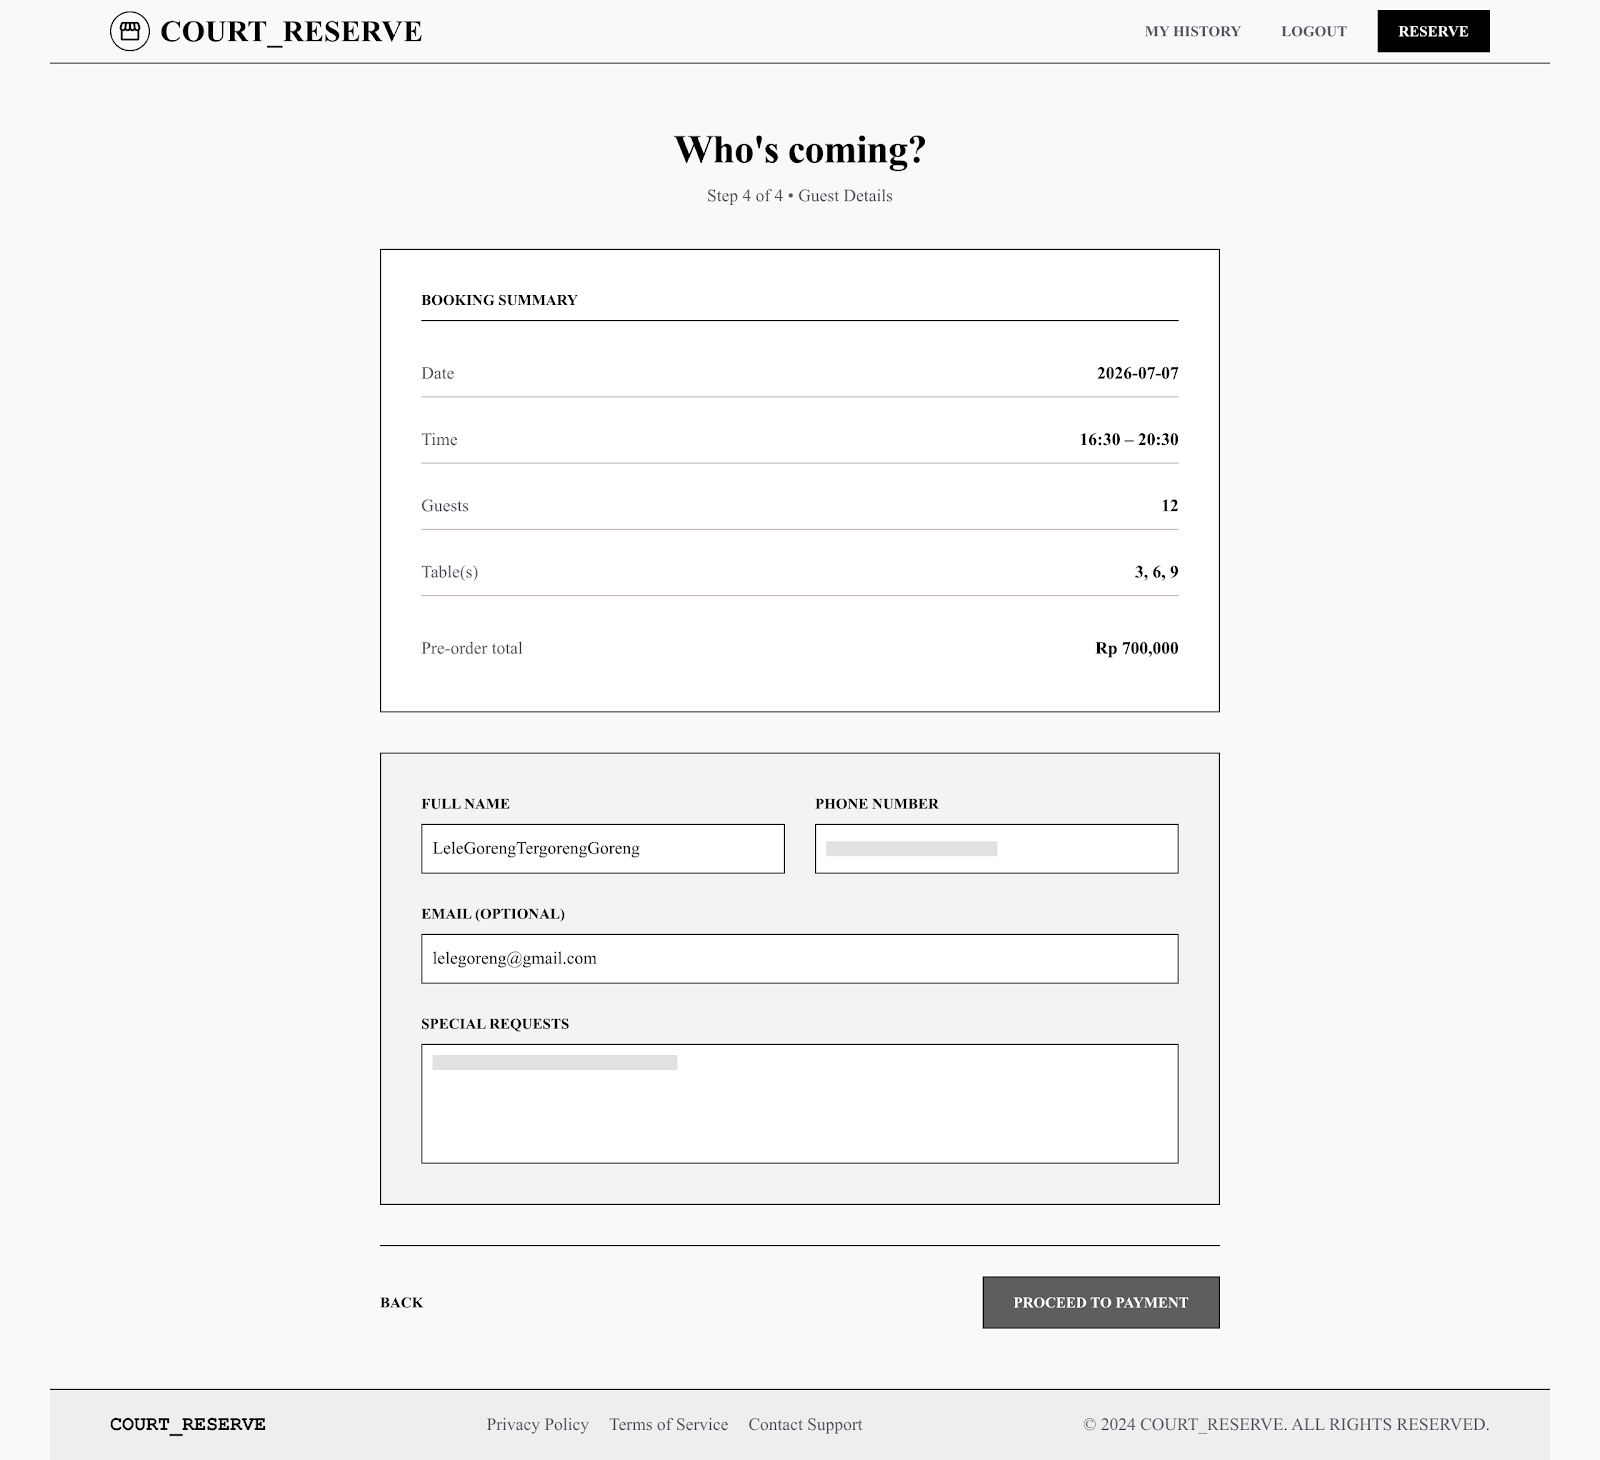
\includegraphics[width=1.0\linewidth]{res/ui_booking_step4_placeholder.png}
    \caption{Rancangan Antarmuka - Tahap 4 Finalisasi}
    \label{fig:ui_step4}
\end{figure}

\subsubsection{Halaman Riwayat Pelanggan}
Halaman profil di mana pelanggan yang sudah masuk (\textit{login}) dapat melihat status pesanan aktif maupun melihat kembali reservasi mereka sebelumnya.
\begin{figure}[htbp]
    \centering
    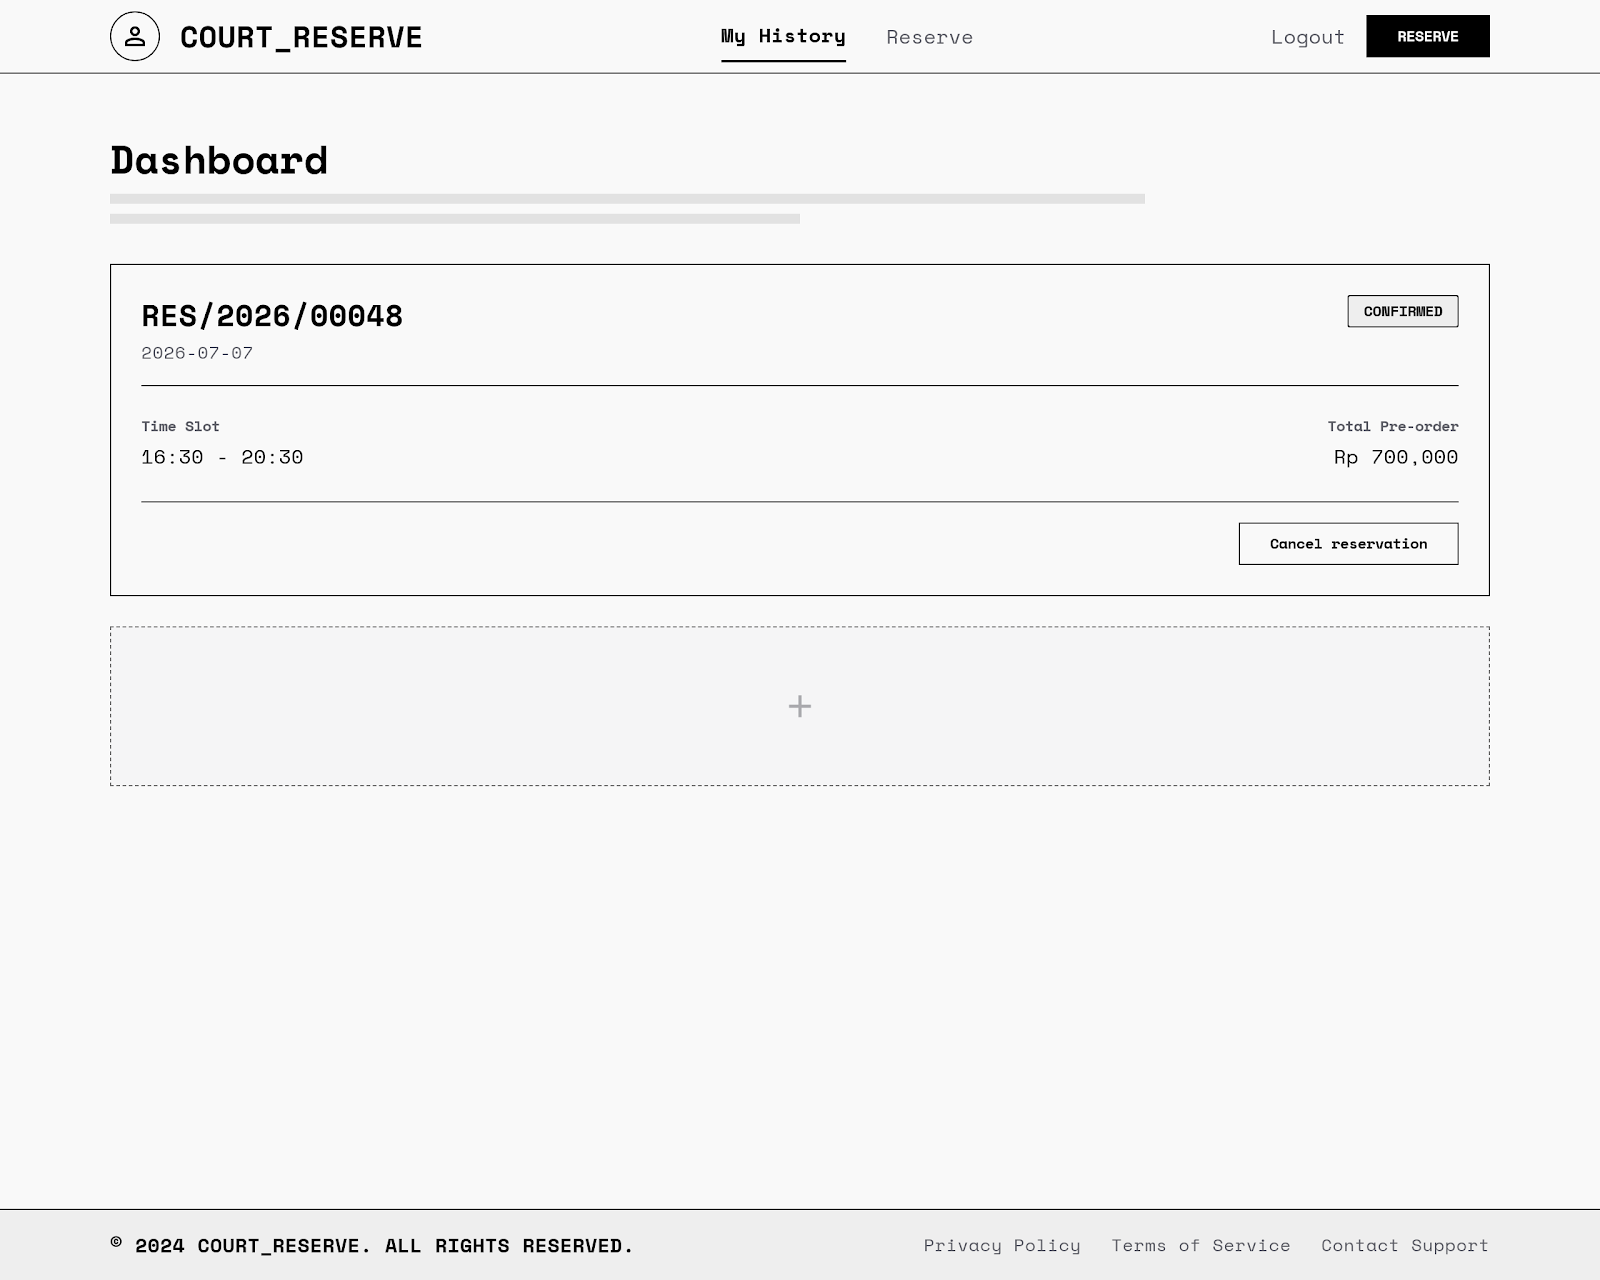
\includegraphics[width=1.0\linewidth]{res/ui_history_placeholder.png}
    \caption{Rancangan Antarmuka Halaman Riwayat Pelanggan}
    \label{fig:ui_history}
\end{figure}

\subsubsection{Visualisasi Data Analitik (Odoo Backend)}
Sistem ini tidak memisahkan antarmuka analitik secara eksternal, melainkan memanfaatkan fitur pelaporan internal bawaan dari \textit{custom module} Odoo. Visualisasi data dirancang untuk menyajikan beberapa metrik utama bagi pihak manajemen:
\begin{itemize}
    \item \textbf{Grafik Okupansi Meja (\textit{Bar Chart}):} Memvisualisasikan persentase penggunaan meja berdasarkan jam atau hari tertentu, berguna untuk mengidentifikasi jam-jam sibuk (\textit{peak hours}).
    \item \textbf{Kontribusi Penjualan Tenant (\textit{Pie Chart}):} Menampilkan perbandingan proporsi pesanan masuk untuk masing-masing tenant, membantu manajemen menilai tenant dengan performa terbaik.
    \item \textbf{Tren Reservasi (\textit{Line Chart}):} Menggambarkan tren jumlah reservasi yang masuk dari waktu ke waktu (harian/mingguan), digunakan sebagai basis prediksi logistik operasional.
    \item \textbf{Ringkasan Pendapatan (\textit{Scorecard}):} Berupa angka metrik (\textit{Key Performance Indicator}) yang menampilkan total pendapatan keseluruhan \textit{food court} maupun pendapatan spesifik tenant.
\end{itemize}
\section{IMPLEMENTASI}

\subsection{Teknologi yang Digunakan}
Implementasi sistem ini memanfaatkan dua tumpukan teknologi (\textit{technology stack}) yang berjalan secara terpisah namun terhubung melalui API. Teknologi-teknologi yang digunakan pada masing-masing sisi adalah sebagai berikut:

\subsubsection{Backend (Odoo ERP)}
\begin{itemize}
    \item \textbf{Odoo 19:} Digunakan sebagai platform ERP utama. Versi 19 digunakan karena mendukung pendekatan \texttt{model.Constraint} berbasis kelas dan metode \texttt{@api.model\_create\_multi} yang lebih efisien untuk operasi \textit{batch create}.
    \item \textbf{Python:} Bahasa pemrograman utama untuk pengembangan modul kustom Odoo, termasuk logika bisnis, \textit{state machine} reservasi, dan pemrosesan \textit{cronjob} otomatis.
    \item \textbf{PostgreSQL:} Sistem manajemen basis data relasional yang digunakan oleh Odoo sebagai penyimpanan data utama.
\end{itemize}

\subsubsection{Frontend (Web Application)}
\begin{itemize}
    \item \textbf{Next.js 16.2:} \textit{Framework} React yang digunakan sebagai fondasi aplikasi web pelanggan. Memanfaatkan fitur \textit{App Router} dan \textit{API Routes} untuk membangun antarmuka yang responsif sekaligus \textit{backend} ringan di sisi server.
    \item \textbf{React 19 \& TypeScript:} Digunakan untuk membangun komponen antarmuka yang bersifat \textit{type-safe} dan mudah dirawat.
    \item \textbf{Tailwind CSS 4 \& Shadcn/UI:} Digunakan untuk membangun antarmuka pengguna yang konsisten dan modern dengan kecepatan tinggi.
    \item \textbf{xmlrpc (npm):} Pustaka JavaScript yang digunakan untuk membangun klien XML-RPC di sisi Next.js, sehingga dapat berkomunikasi langsung dengan \textit{endpoint} Odoo.
\end{itemize}

\subsubsection{Layanan Eksternal}
\begin{itemize}
    \item \textbf{Midtrans Snap:} \textit{Payment Gateway} yang diintegrasikan untuk memproses transaksi pembayaran daring. Setelah pelanggan melakukan \textit{pre-order}, sistem Next.js akan membuat transaksi Midtrans dan mengarahkan pelanggan ke halaman pembayaran Midtrans Snap.
\end{itemize}

\subsection{Implementasi Backend (Modul Kustom Odoo)}
Modul kustom bernama \texttt{foodcourt} dikembangkan menggunakan kerangka kerja Odoo dan terdiri dari beberapa model utama.

\subsubsection{Model Manajemen Tenant (\texttt{foodcourt.tenant})}
Model ini mengelola seluruh siklus hidup penyewa (\textit{tenant}) yang beroperasi di dalam \textit{food court}. Model ini mewarisi \texttt{mail.thread} untuk mendukung pencatatan aktivitas dan notifikasi internal. Atribut utamanya mencakup nama tenant, kode unik yang digenerate otomatis melalui \textit{sequence}, jenis masakan (\textit{cuisine\_type}), persentase bagi hasil pendapatan (\textit{revenue\_share\_pct}), dan status kontrak yang dikelola melalui \textit{state machine}: \texttt{draft} $\rightarrow$ \texttt{active} $\rightarrow$ \texttt{suspended} / \texttt{terminated}.

Fitur analitik untuk tenant diimplementasikan melalui metode \textit{compute}:
\begin{itemize}
    \item \texttt{\_compute\_order\_count}: Menghitung total pesanan masuk dengan mencari rekaman \texttt{pos.order.line} yang memiliki \textit{foreign key} ke tenant tersebut.
    \item \texttt{\_compute\_total\_revenue}: Menjumlahkan \texttt{price\_subtotal} dari seluruh baris pesanan POS dengan status \texttt{paid}, \texttt{done}, atau \texttt{invoiced}.
\end{itemize}

\subsubsection{Model Reservasi (\texttt{foodcourt.reservation})}
Ini adalah model inti dari sistem. Model ini mengimplementasikan alur \textit{state machine} yang lengkap dengan tujuh kondisi status:

\begin{center}
\texttt{draft} $\rightarrow$ \texttt{pending\_payment} $\rightarrow$ \texttt{confirmed} $\rightarrow$ \texttt{checked\_in} $\rightarrow$ \texttt{completed}
\end{center}

dengan cabang pembatalan ke \texttt{cancelled} atau \texttt{no\_show}.

Fitur-fitur kunci yang diimplementasikan pada model ini adalah:
\begin{itemize}
    \item \textbf{Pencegahan Pemesanan Ganda (\textit{Double-Booking Prevention}):} Diimplementasikan melalui metode \texttt{\_check\_table\_availability()}. Sistem melakukan kueri pencarian reservasi yang tumpang-tindih (\textit{overlapping}) berdasarkan tanggal yang sama, meja yang sama, waktu yang beririsan, serta status yang masih aktif (\texttt{pending\_payment}, \texttt{confirmed}, atau \texttt{checked\_in}).
    \item \textbf{Pembuatan Pesanan POS Otomatis:} Saat admin melakukan \textit{check-in} tamu (\texttt{action\_check\_in}), sistem secara otomatis memanggil metode \texttt{\_create\_pos\_order\_from\_reservation()}. Metode ini mencari sesi POS yang sedang aktif, kemudian membuat rekaman \texttt{pos.order} baru beserta baris-baris pesanannya berdasarkan data \textit{pre-order} yang telah diisi pelanggan sebelumnya.
    \item \textbf{Bidang Kalender:} Dua bidang \texttt{date\_start} dan \texttt{date\_stop} dikomputasi secara otomatis dari kombinasi \texttt{reservation\_date} dan \texttt{time\_start}/\texttt{time\_end} untuk memungkinkan tampilan kalender di Odoo.
    \item \textbf{Notifikasi E-mail:} Sistem mengirimkan e-mail konfirmasi secara otomatis saat reservasi dikonfirmasi, menggunakan \textit{template} e-mail yang didefinisikan di dalam modul.
\end{itemize}

\subsubsection{Proses Otomatis (\textit{Cron Jobs})}
Tiga \textit{cronjob} diimplementasikan untuk menjaga integritas data secara otomatis tanpa intervensi manual:
\begin{itemize}
    \item \textbf{\texttt{\_cron\_cancel\_pending\_payments}:} Membatalkan secara otomatis reservasi yang berstatus \texttt{pending\_payment} apabila telah melewati batas waktu 15 menit. Mekanisme ini mencegah meja terkunci selamanya akibat pembayaran yang tidak diselesaikan.
    \item \textbf{\texttt{\_cron\_cancel\_expired\_reservations}:} Mengubah status reservasi yang sudah dikonfirmasi menjadi \texttt{no\_show} apabila 15 menit telah berlalu sejak waktu kedatangan yang dijadwalkan namun tamu belum melakukan \textit{check-in}.
    \item \textbf{\texttt{\_cron\_send\_reminder\_emails}:} Mengirimkan e-mail pengingat kepada pelanggan yang memiliki reservasi aktif dalam 3 jam ke depan.
\end{itemize}

\subsection{Implementasi Integrasi API}
Lapisan integrasi antara Next.js dan Odoo diimplementasikan menggunakan modul \texttt{xmlrpc} bawaan Odoo, yang diakses dari sisi Next.js menggunakan paket \texttt{xmlrpc} dari npm. Klien XML-RPC tersebut dibungkus dalam sebuah \textit{singleton utility} bernama \texttt{odooClient} yang mengabstraksi detail koneksi (\textit{host}, \textit{port}, \textit{database}, \textit{username}, dan \textit{password}) sehingga dapat digunakan kembali di seluruh \textit{API Route} Next.js.

Seluruh komunikasi ke Odoo dilakukan melalui \textit{API Route} Next.js yang berperan sebagai \textit{proxy} keamanan, sehingga kredensial dan detail Odoo tidak pernah terekspos ke sisi klien. Tabel~\ref{tab:api_routes} merangkum rute-rute API yang diimplementasikan:

\begin{table}[htbp]
\caption{Daftar API Route Implementasi Next.js}
\label{tab:api_routes}
\centering
\begin{tabularx}{\linewidth}{|p{3.2cm}|c|X|}
\hline
\textbf{Endpoint} & \textbf{Metode} & \textbf{Fungsi} \\
\hline
\url{/api/tables} & GET & Mengambil daftar meja yang tersedia dari Odoo berdasarkan parameter tanggal, jam mulai, dan jam selesai. \\
\hline
\url{/api/floor} & GET & Mengambil metadata denah lantai (\textit{floor plan}) termasuk gambar latar belakang untuk komponen peta interaktif. \\
\hline
\url{/api/menu} & GET & Mengambil seluruh daftar menu makanan yang tersedia di POS beserta informasi tenant masing-masing. \\
\hline
\url{/api/reservations} & POST & Membuat reservasi baru di Odoo. Jika ada \textit{pre-order}, sistem membuat transaksi Midtrans dan mengembalikan \textit{URL} pembayaran. \\
\hline
\url{/api/reservations/cancel} & POST & Membatalkan reservasi yang dimiliki pengguna yang sedang \textit{login}. \\
\hline
\url{/api/auth/session} & GET & Memvalidasi \textit{cookie} sesi pengguna yang aktif dan mengembalikan data profil. \\
\hline
\url{/api/register} & POST & Mendaftarkan akun pelanggan baru sekaligus membuat kontak (\textit{res.partner}) baru di Odoo. \\
\hline
\url{/api/webhooks} & POST & Menerima notifikasi dari Midtrans untuk memperbarui status pembayaran reservasi di Odoo. \\
\hline
\end{tabularx}
\end{table}

\subsection{Implementasi Fitur Utama}

\subsubsection{Alur Pemesanan Multi-Langkah (\textit{Multi-step Booking})}
Fitur pemesanan diimplementasikan sebagai satu halaman (\texttt{/book}) menggunakan pendekatan \textit{state machine} sederhana di sisi klien melalui variabel \texttt{step} yang dikelola dengan \texttt{useState}. Halaman ini terdiri dari empat tahap yang ditampilkan secara kondisional.

Untuk mencegah kehilangan data saat pelanggan tamu diarahkan ke halaman registrasi, sistem mengimplementasikan mekanisme \textit{state persistence} menggunakan \texttt{localStorage}. Seluruh data formulir yang telah diisi (tanggal, jam, meja yang dipilih, \textit{pre-order}) disimpan sementara ke \texttt{localStorage} sebelum pengalihan halaman, kemudian dipulihkan secara otomatis setelah pengguna berhasil mendaftar dan dikembalikan ke halaman pemesanan.

\subsubsection{Peta Denah Lantai Interaktif (\textit{Interactive Floor Map})}
Pada Tahap 2, ketersediaan meja divisualisasikan menggunakan komponen \texttt{FloorMap} yang merender posisi dan dimensi meja berdasarkan data spasial (\texttt{position\_h}, \texttt{position\_v}, \texttt{width}, \texttt{height}) yang diambil langsung dari Odoo. Komponen ini mendukung fitur \textit{pan} (geser) dan \textit{zoom} (perbesar) untuk kemudahan navigasi pada denah yang kompleks.

\subsubsection{Integrasi Pembayaran (Midtrans Snap)}
Ketika pelanggan melakukan \textit{pre-order} makanan, total tagihan dihitung oleh Odoo (sumber data yang otoritatif), bukan oleh Next.js, untuk mencegah manipulasi harga di sisi klien. Sistem kemudian membuat transaksi di Midtrans menggunakan \textit{Server Key} yang tersimpan di \textit{environment variable} sisi server. Pelanggan diarahkan ke halaman Midtrans Snap untuk menyelesaikan pembayaran. Setelah pembayaran selesai, Midtrans mengirimkan notifikasi ke \textit{endpoint} webhook (\texttt{/api/webhooks}) yang kemudian memperbarui status reservasi di Odoo menjadi \texttt{confirmed}.

\subsubsection{Implementasi Analitik di Odoo}
Fitur analitik diimplementasikan secara langsung di dalam model \texttt{foodcourt.tenant} sebagai \textit{field} yang dikomputasi secara \textit{real-time}. Data ini dapat ditampilkan dalam tampilan \textit{dashboard} Odoo menggunakan blok \texttt{<graph>} dan \texttt{<pivot>} yang didefinisikan dalam \textit{view} XML modul, sehingga memungkinkan admin untuk melihat grafik performa penjualan setiap tenant langsung di dalam antarmuka Odoo tanpa perlu alat analitik pihak ketiga.

\subsection{Hasil Implementasi}
Berikut ini disajikan tangkapan layar (\textit{screenshot}) dari sistem yang telah berjalan, baik dari sisi \textit{Web Frontend} yang diakses pelanggan maupun sisi \textit{Backend} Odoo yang digunakan oleh admin dan operator.

\subsubsection{Tampilan Web Frontend}

\textbf{Halaman Utama (\textit{Homepage}):}
Halaman utama menampilkan identitas visual \textit{Coco Foodcourt} dengan teks sambutan dan tombol CTA (\textit{Reserve a Table}) yang langsung mengarahkan pelanggan ke alur pemesanan.
\begin{figure}[htbp]
    \centering
    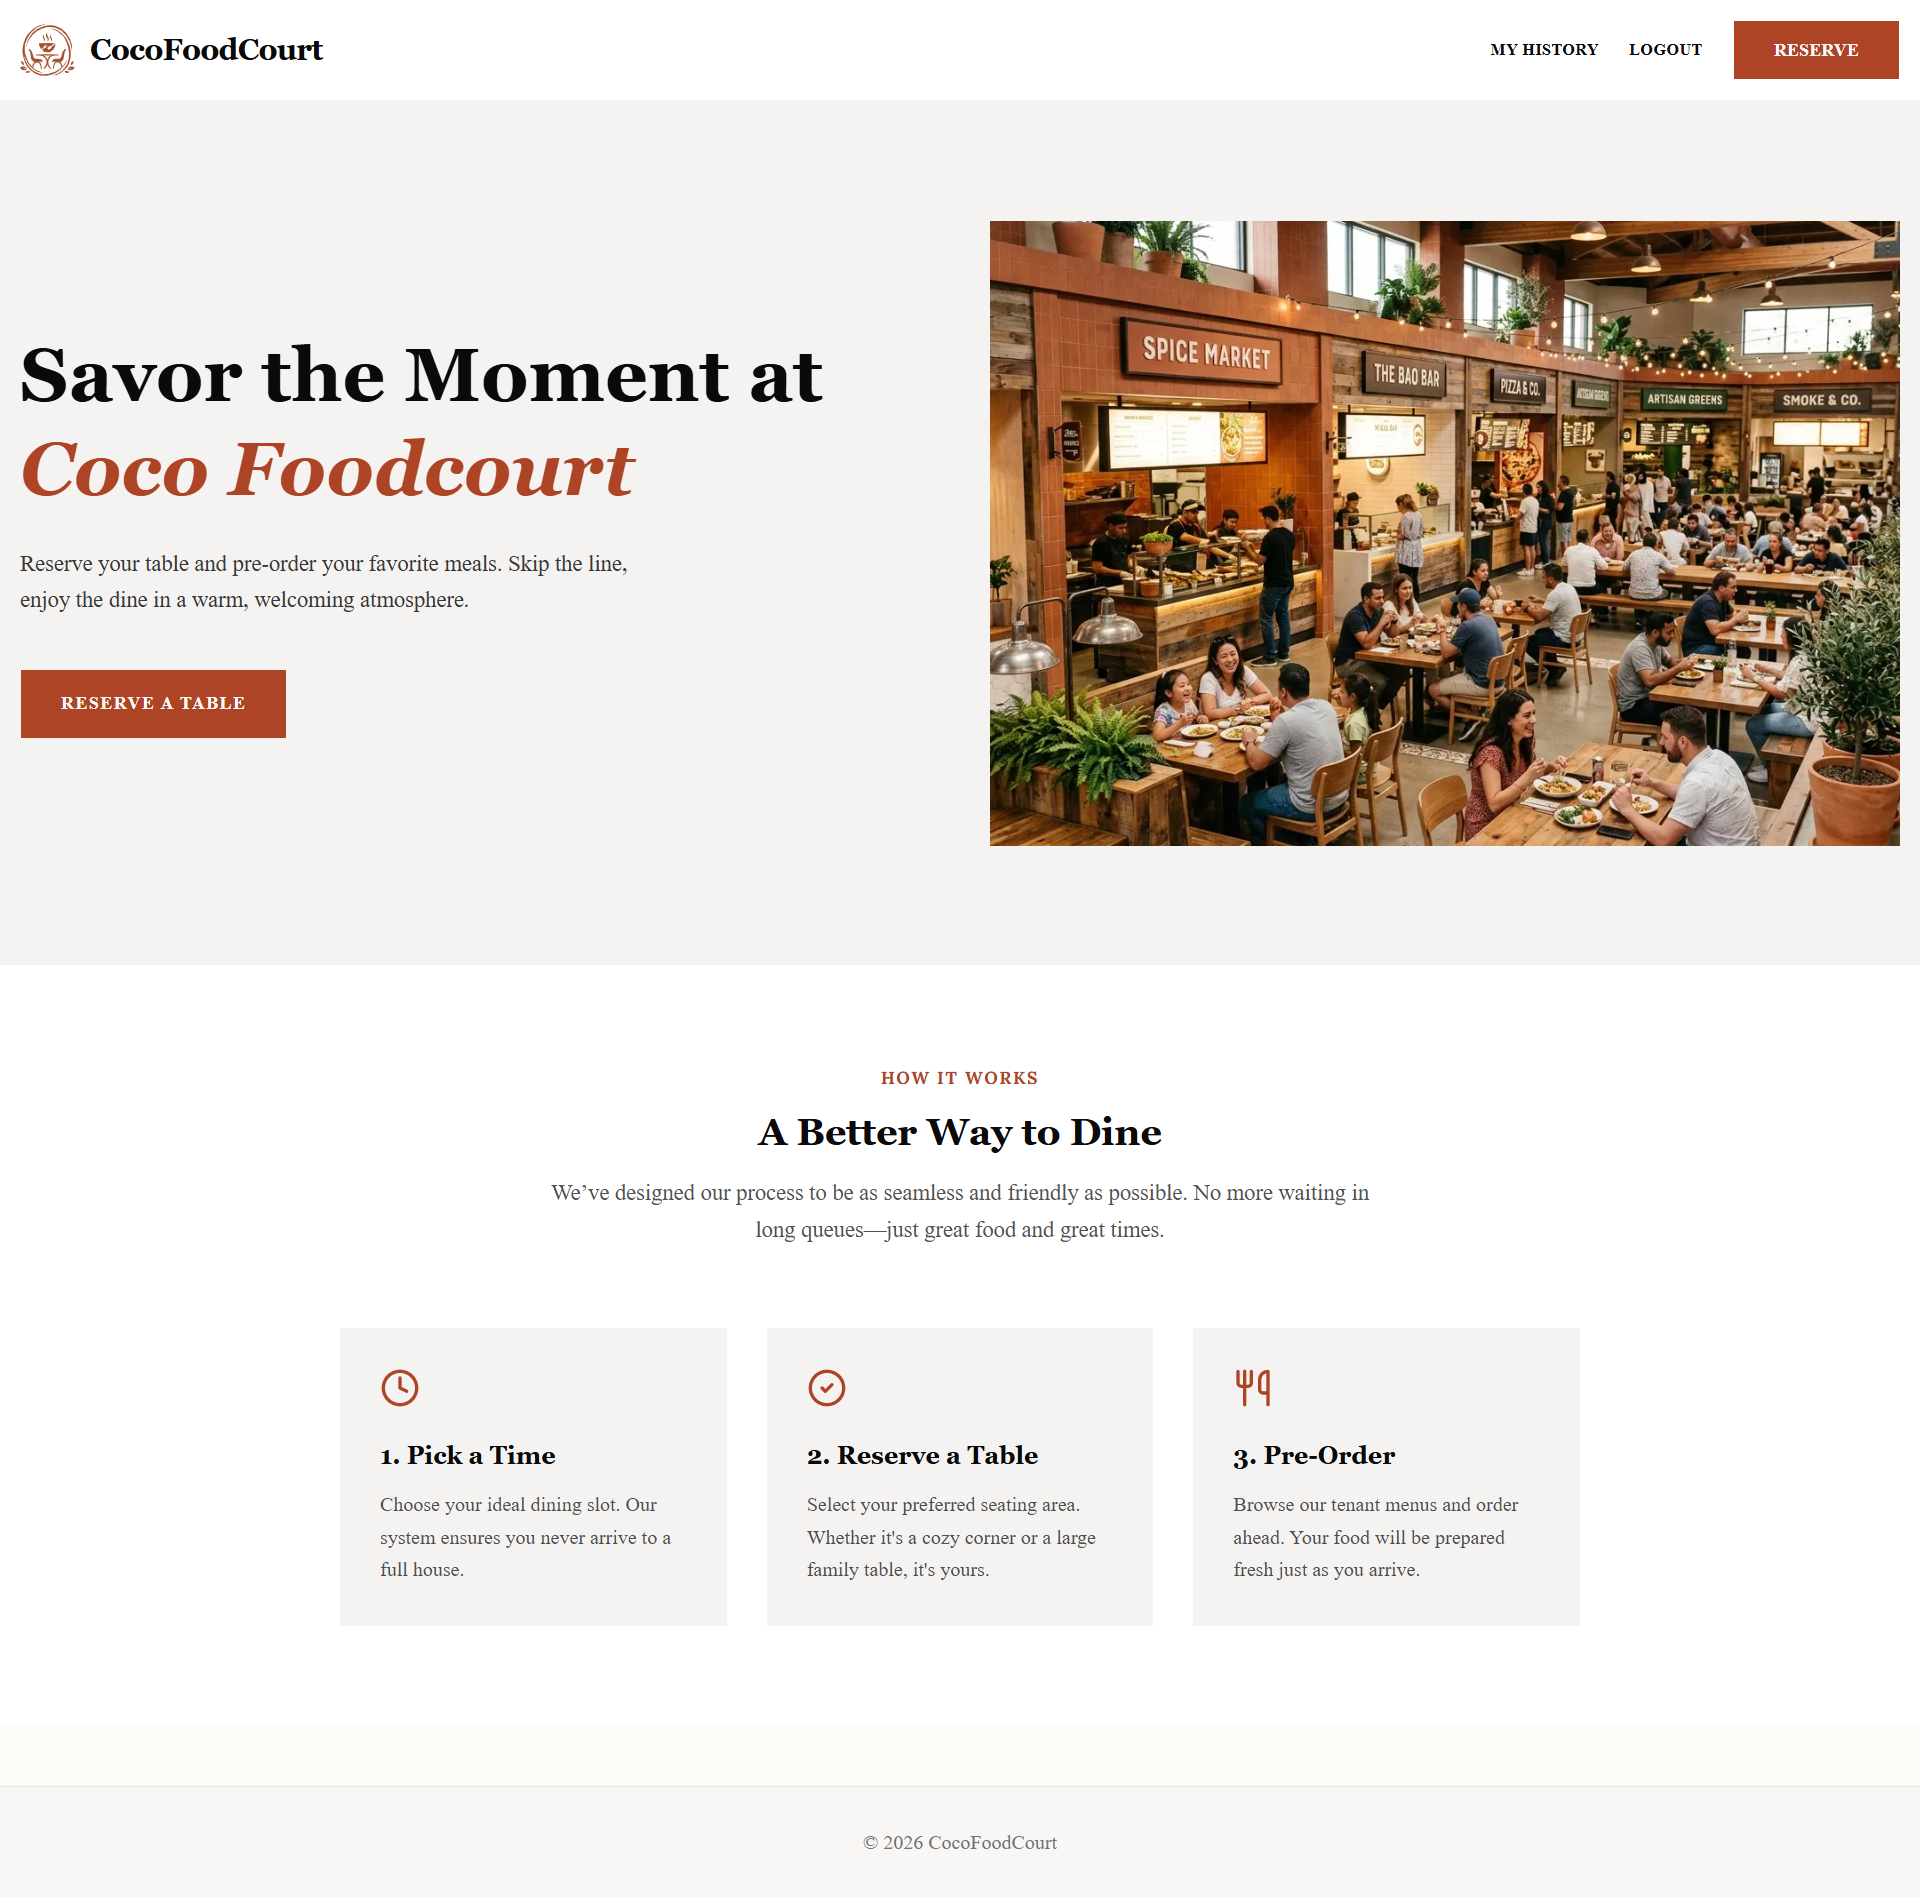
\includegraphics[width=1.0\linewidth]{res/ss_web_homepage.png}
    \caption{Tampilan Halaman Utama Web Frontend}
    \label{fig:ss_homepage}
\end{figure}

\textbf{Tahap 1 - Input Waktu \& Tamu:}
Pelanggan memasukkan tanggal kunjungan, waktu kedatangan, waktu kepulangan, dan jumlah tamu sebelum sistem mencari meja yang tersedia.
\begin{figure}[htbp]
    \centering
    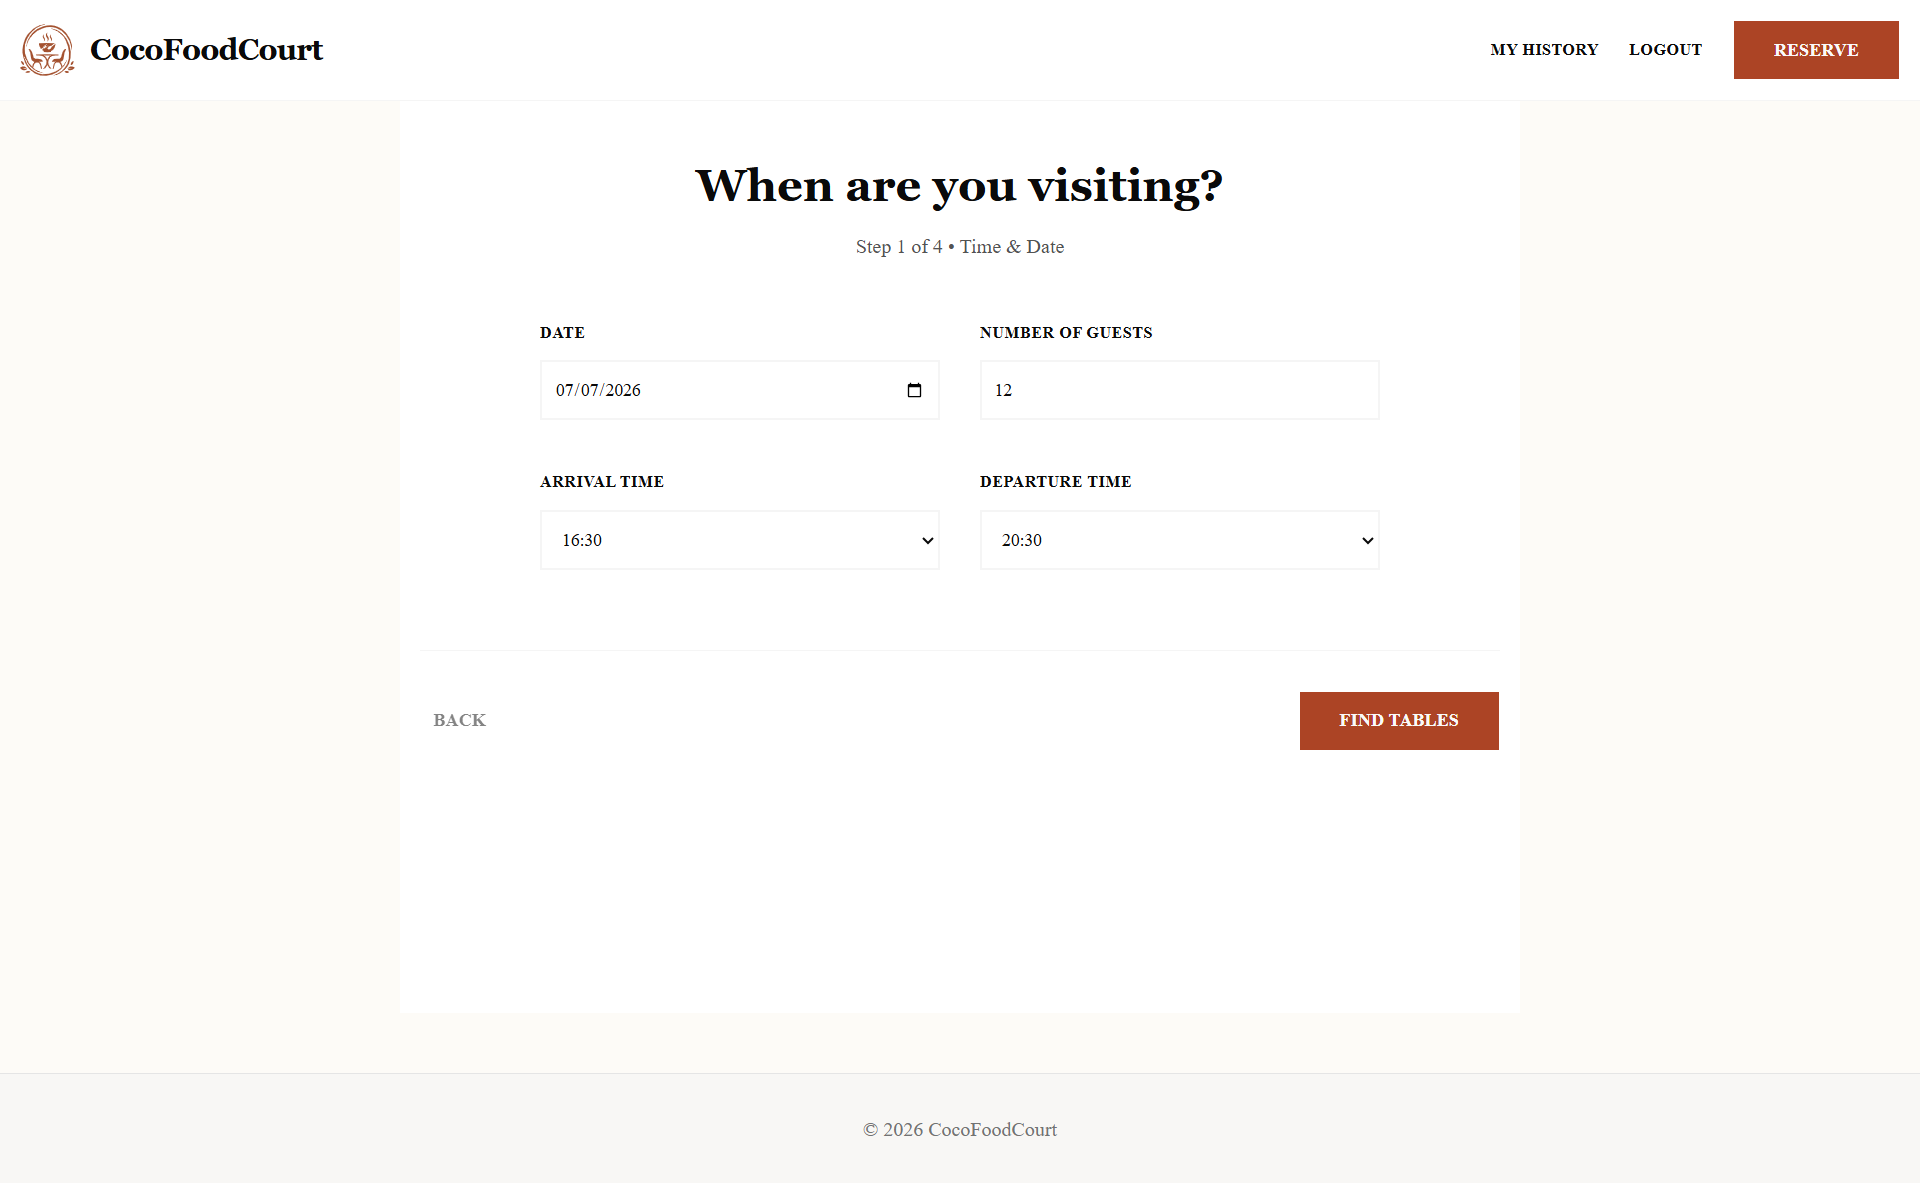
\includegraphics[width=1.0\linewidth]{res/ss_web_step1.png}
    \caption{Tampilan Booking Tahap 1 — Input Waktu dan Jumlah Tamu}
    \label{fig:ss_step1}
\end{figure}

\textbf{Tahap 2 - Pemilihan Meja (Peta Interaktif):}
Sistem menampilkan denah lantai secara interaktif. Meja yang tersedia ditandai dengan warna terang, sedangkan meja yang sudah dipesan ditampilkan dengan warna redup.
\begin{figure}[htbp]
    \centering
    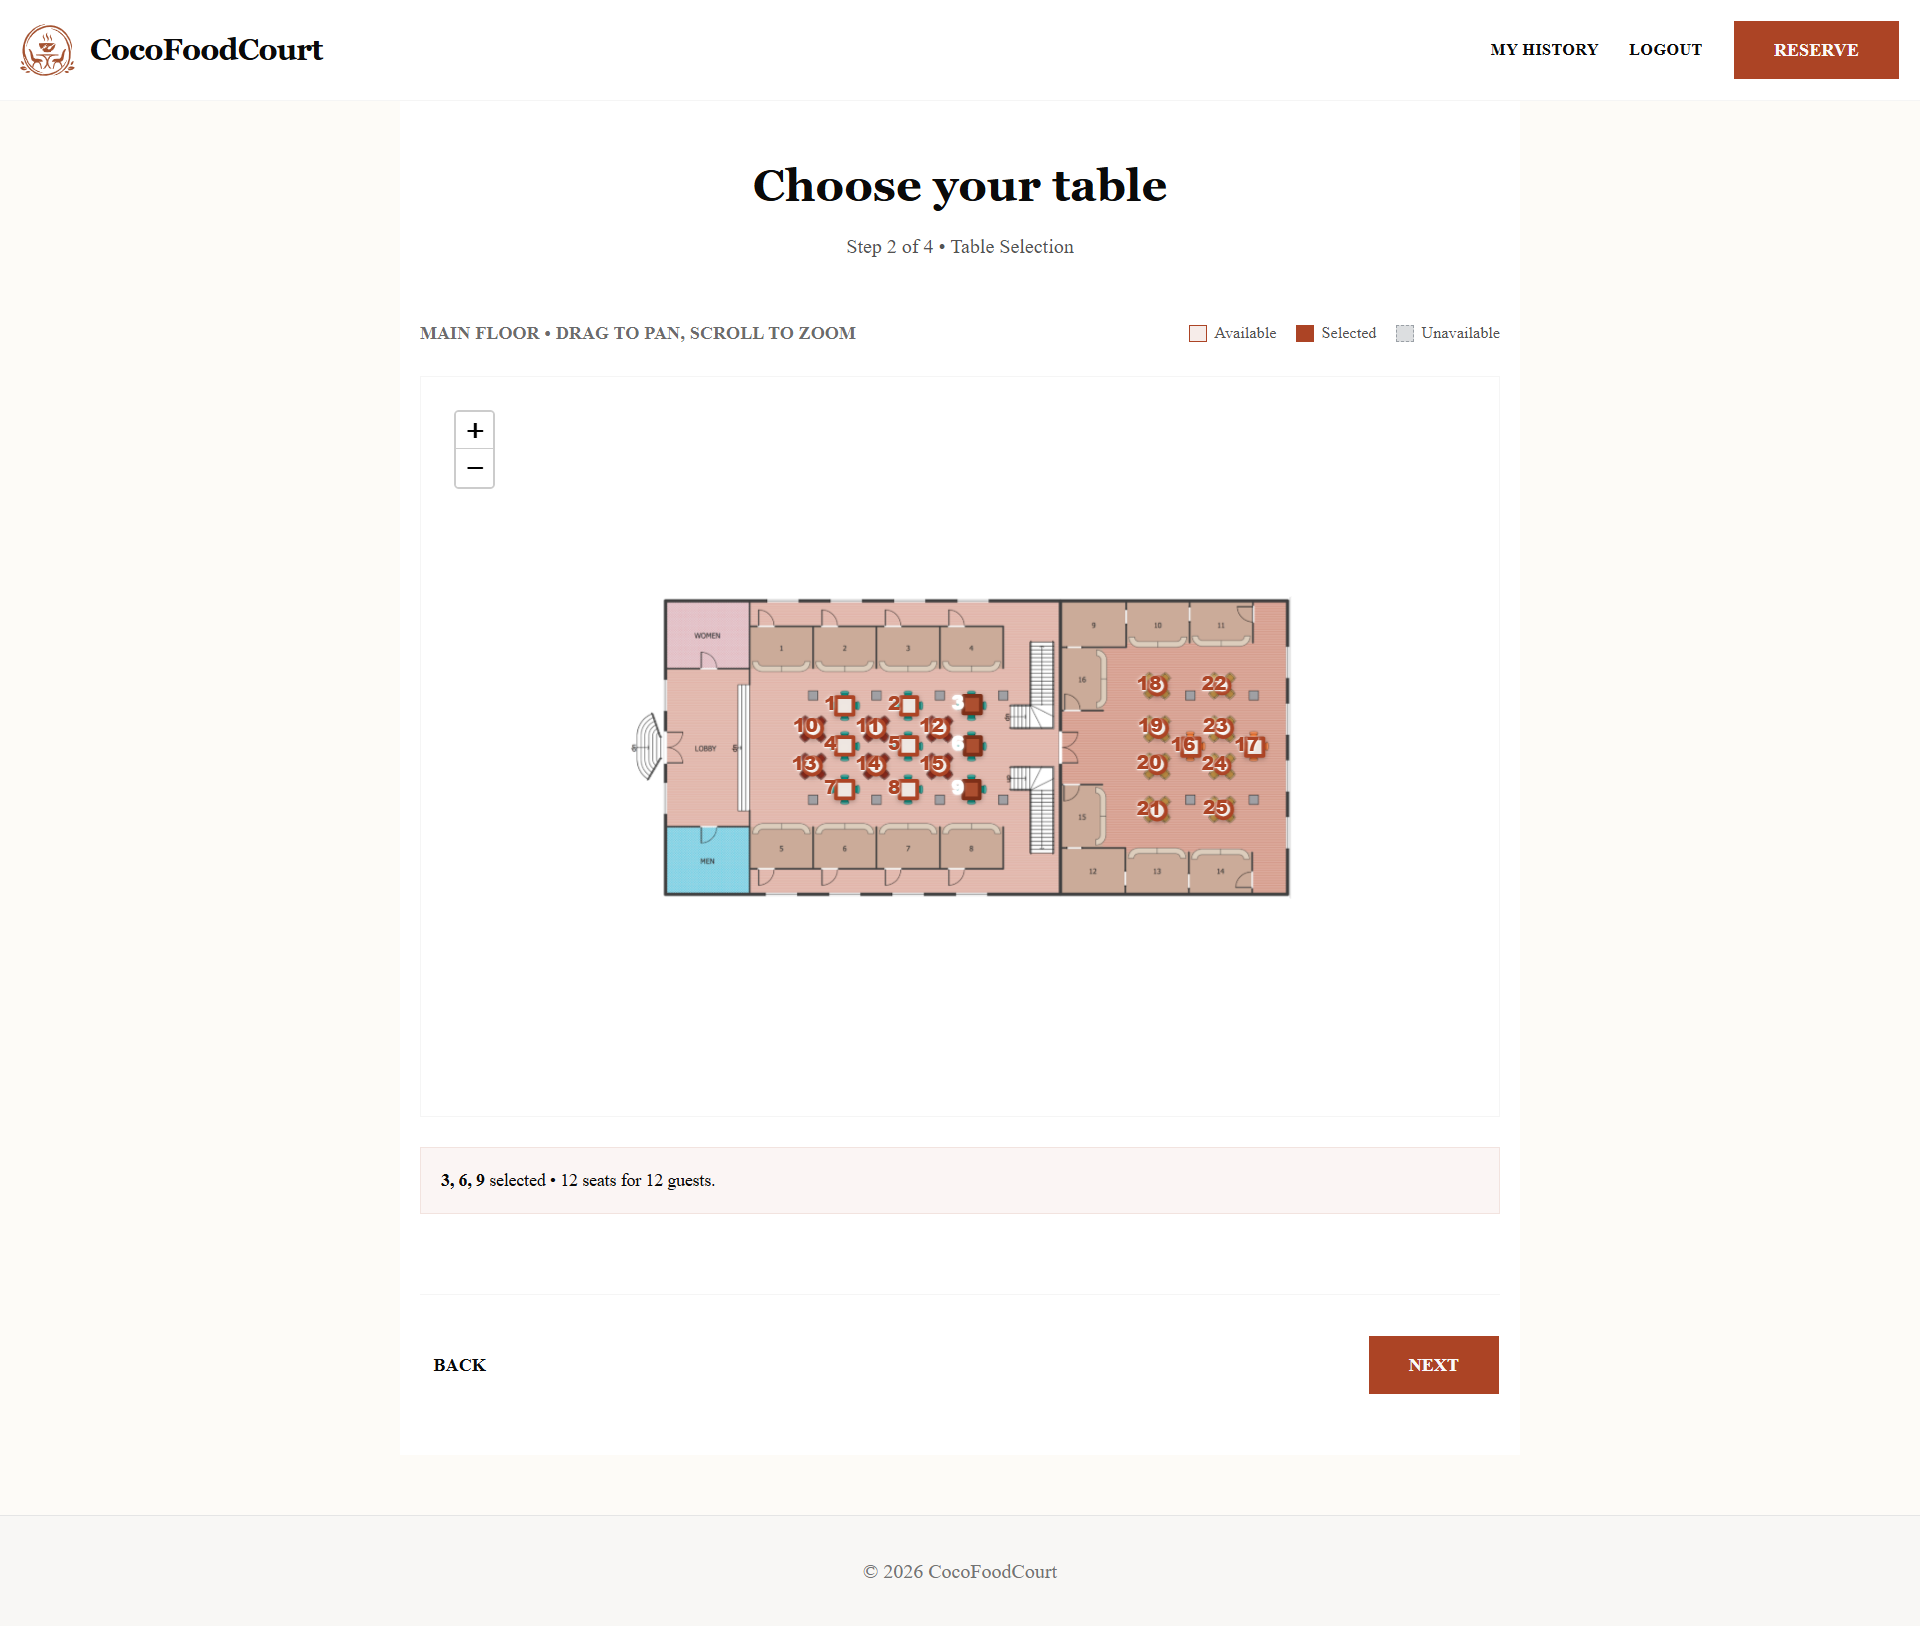
\includegraphics[width=1.0\linewidth]{res/ss_web_step2.png}
    \caption{Tampilan Booking Tahap 2 — Pemilihan Meja pada Peta Interaktif}
    \label{fig:ss_step2}
\end{figure}

\textbf{Tahap 3 - Pemilihan Menu (\textit{Pre-order}):}
Pelanggan memilih menu makanan dari berbagai tenant. Sistem menampilkan daftar menu yang dapat difilter berdasarkan nama atau nama tenant.
\begin{figure}[htbp]
    \centering
    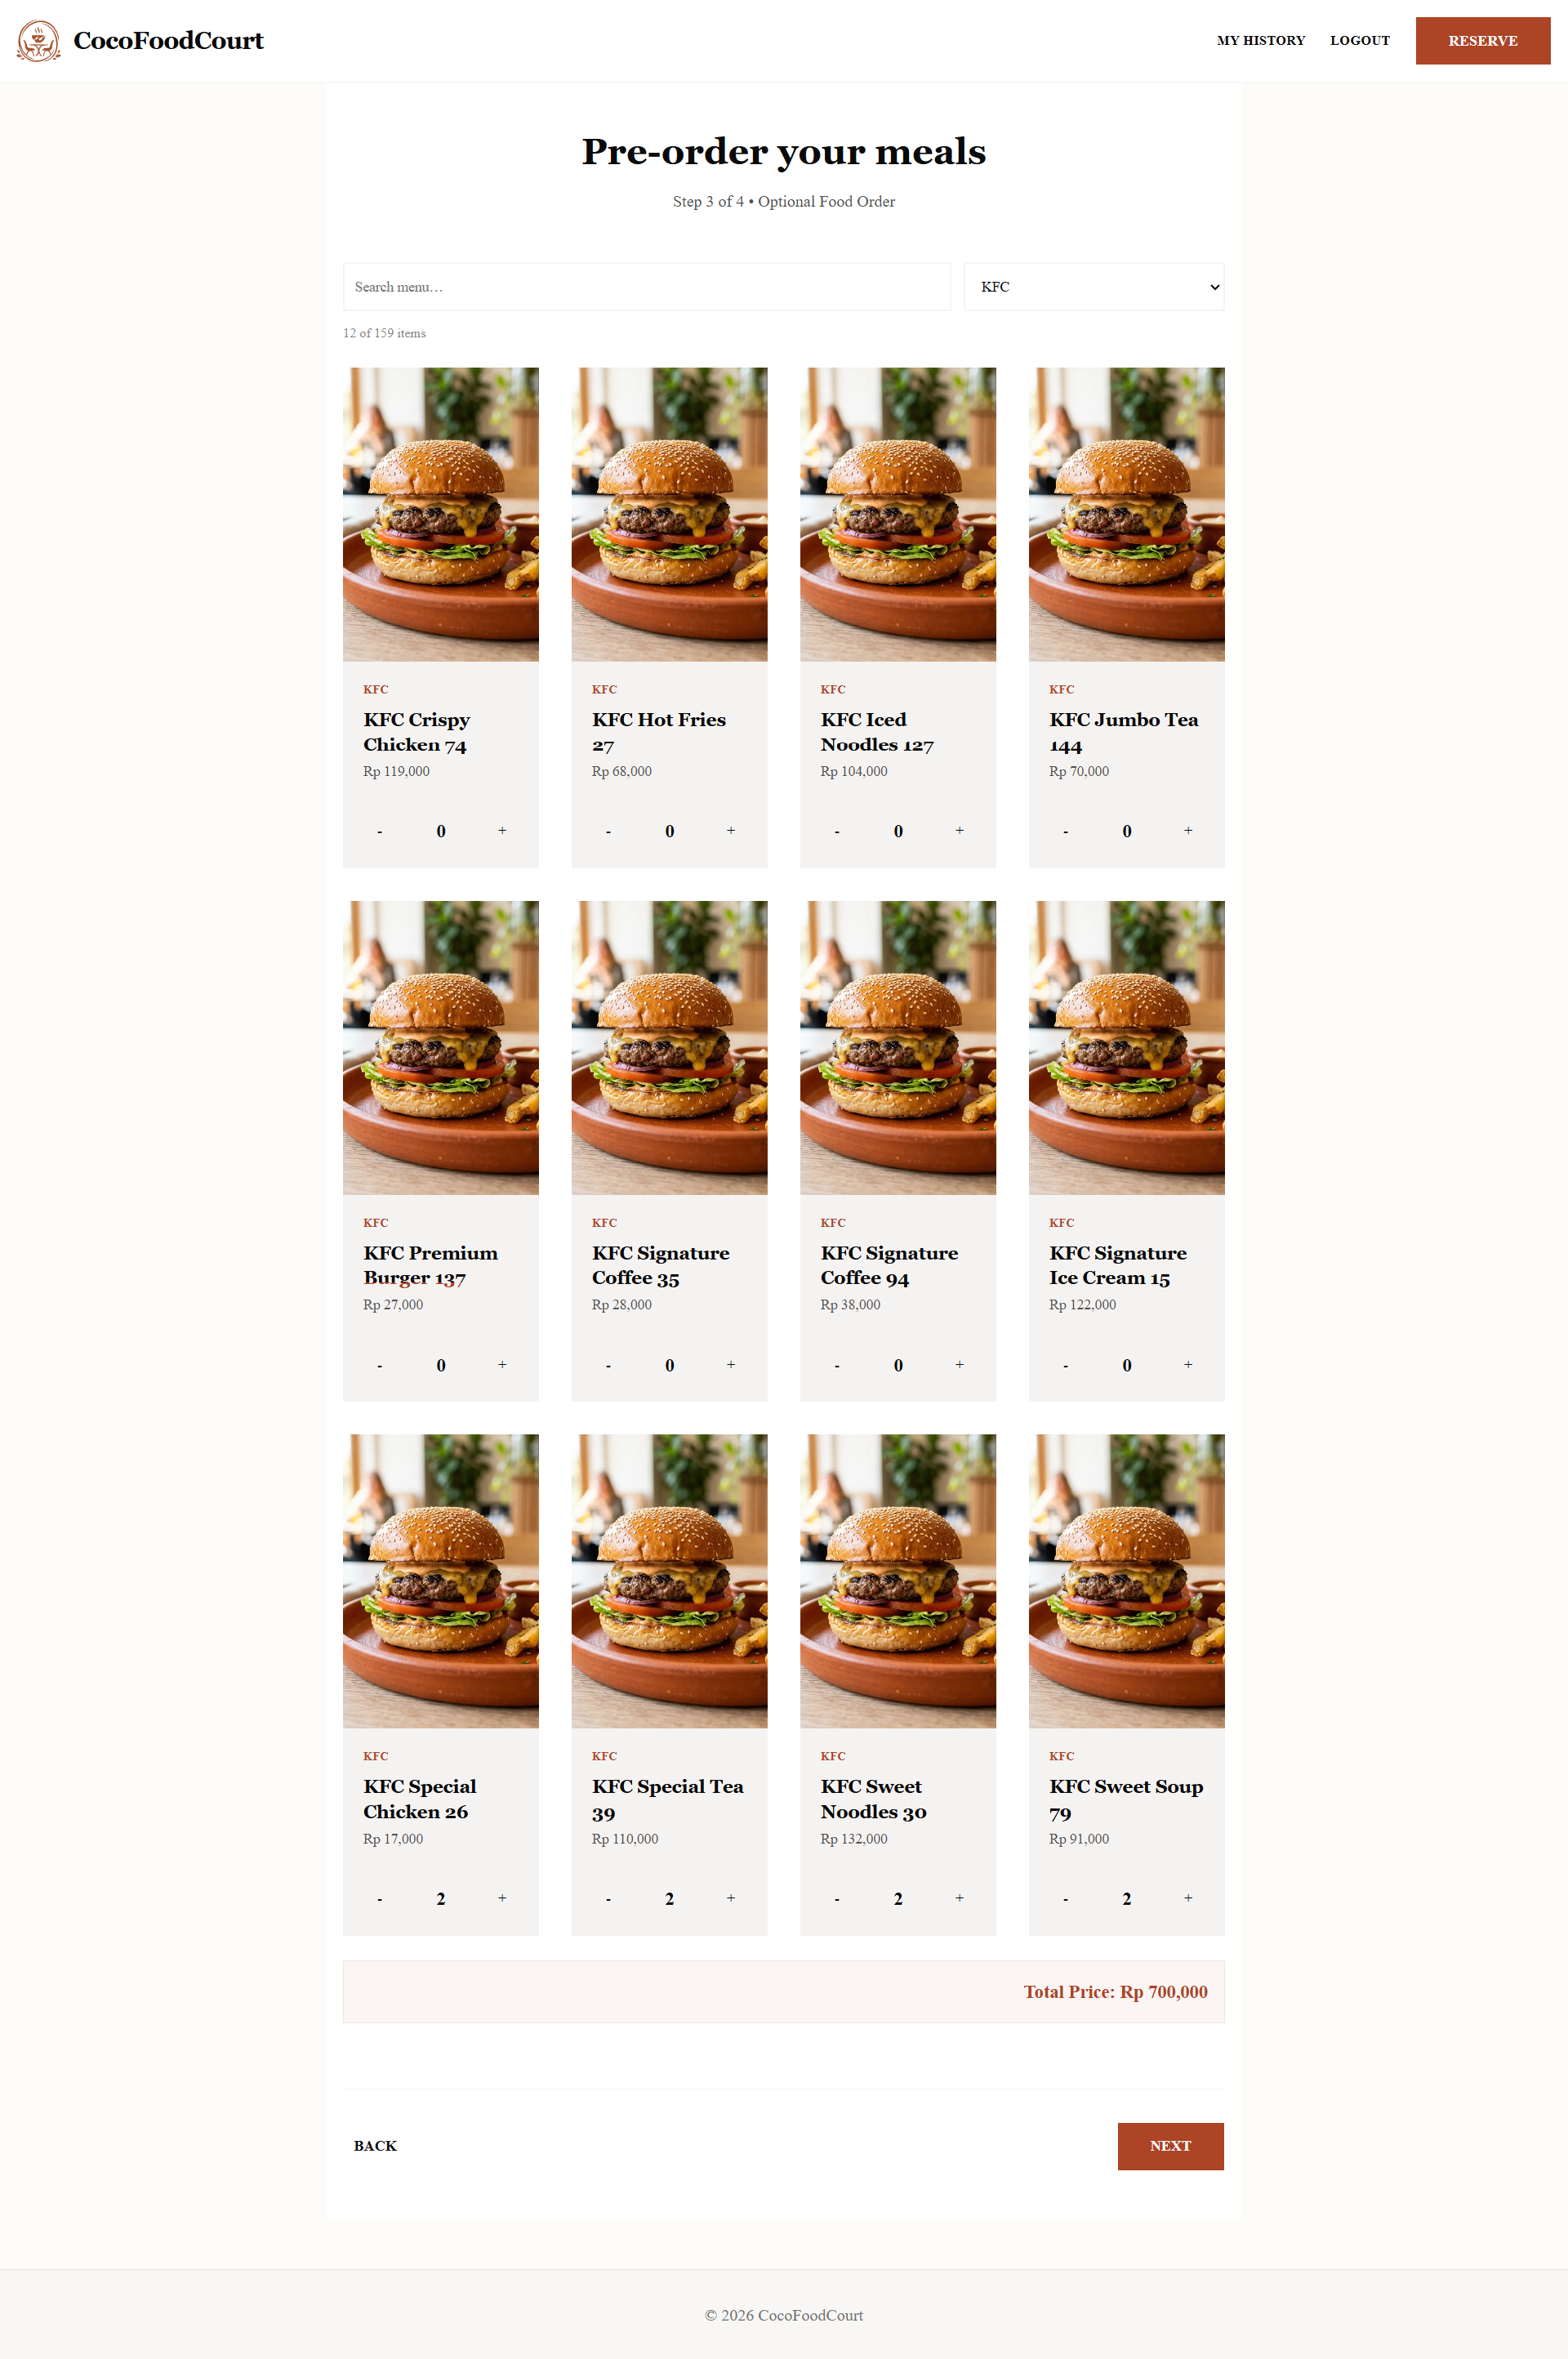
\includegraphics[width=1.0\linewidth]{res/ss_web_step3.png}
    \caption{Tampilan Booking Tahap 3 — Pemilihan Menu \textit{Pre-order}}
    \label{fig:ss_step3}
\end{figure}

\textbf{Tahap 4 - Finalisasi \& Konfirmasi:}
Halaman finalisasi menampilkan ringkasan reservasi secara menyeluruh, formulir data diri, dan tombol konfirmasi. Jika ada \textit{pre-order}, sistem mengarahkan pelanggan ke pembayaran Midtrans Snap.
\begin{figure}[htbp]
    \centering
    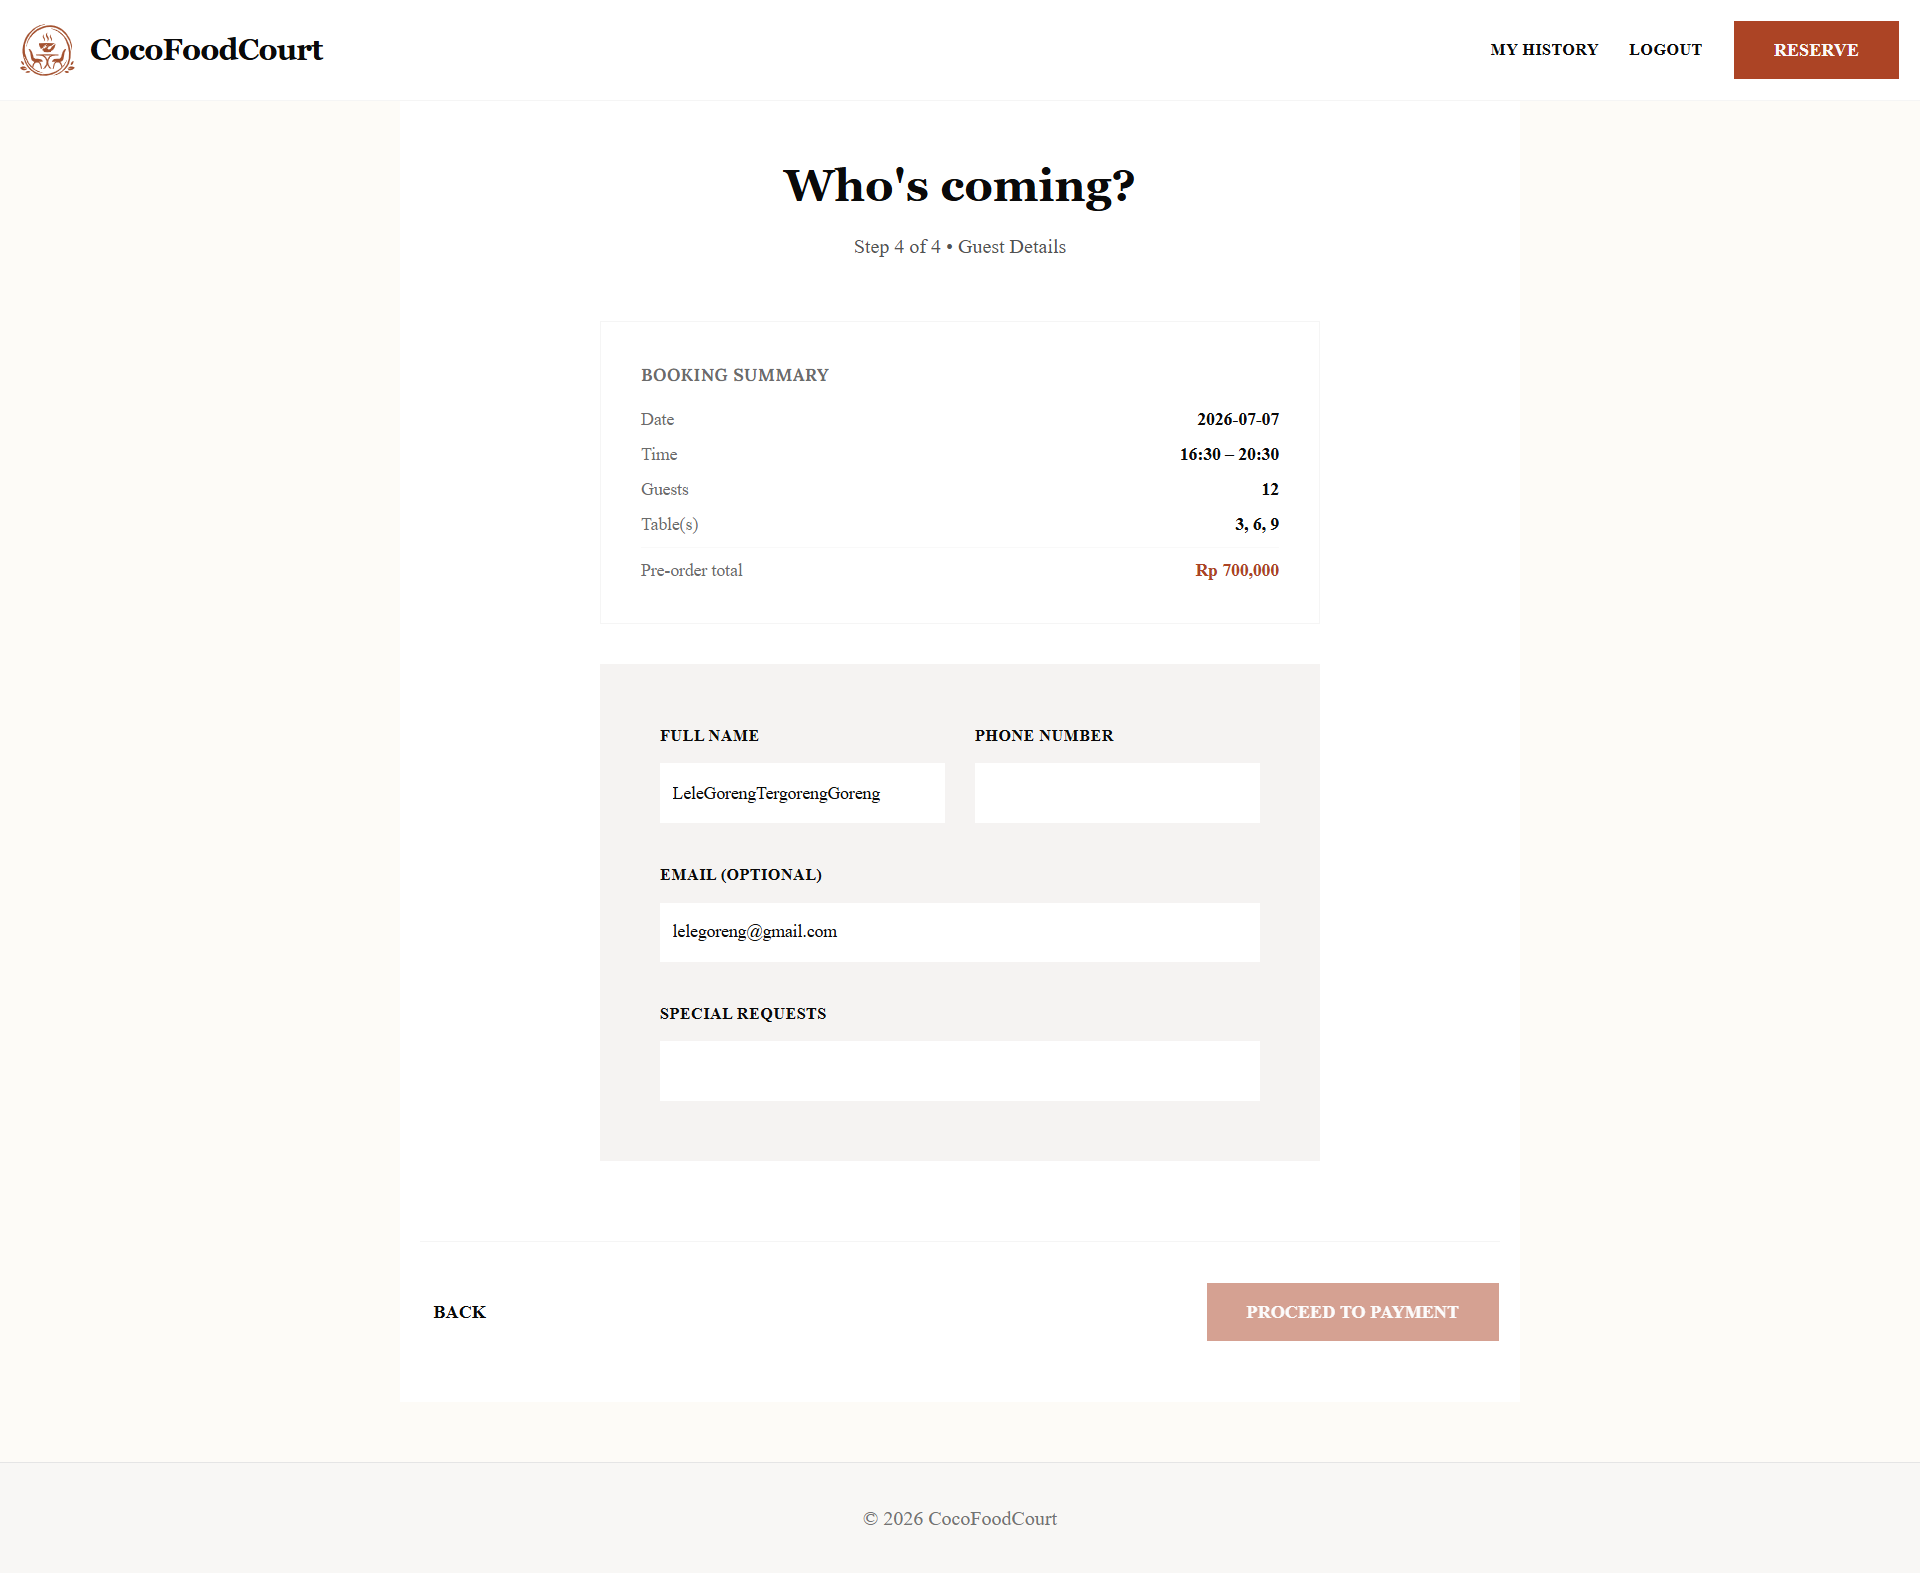
\includegraphics[width=1.0\linewidth]{res/ss_web_step4.png}
    \caption{Tampilan Booking Tahap 4 — Finalisasi dan Konfirmasi}
    \label{fig:ss_step4}
\end{figure}

\textbf{Tahap 5 - Pembayaran:}
Halaman ini menampilkan \textit{popup} antarmuka pembayaran dari Midtrans Snap. Pelanggan dapat menyelesaikan transaksi \textit{pre-order} dengan memindai kode QRIS atau menggunakan metode pembayaran lain yang tersedia sebelum batas waktu habis.
\begin{figure}[htbp]
    \centering
    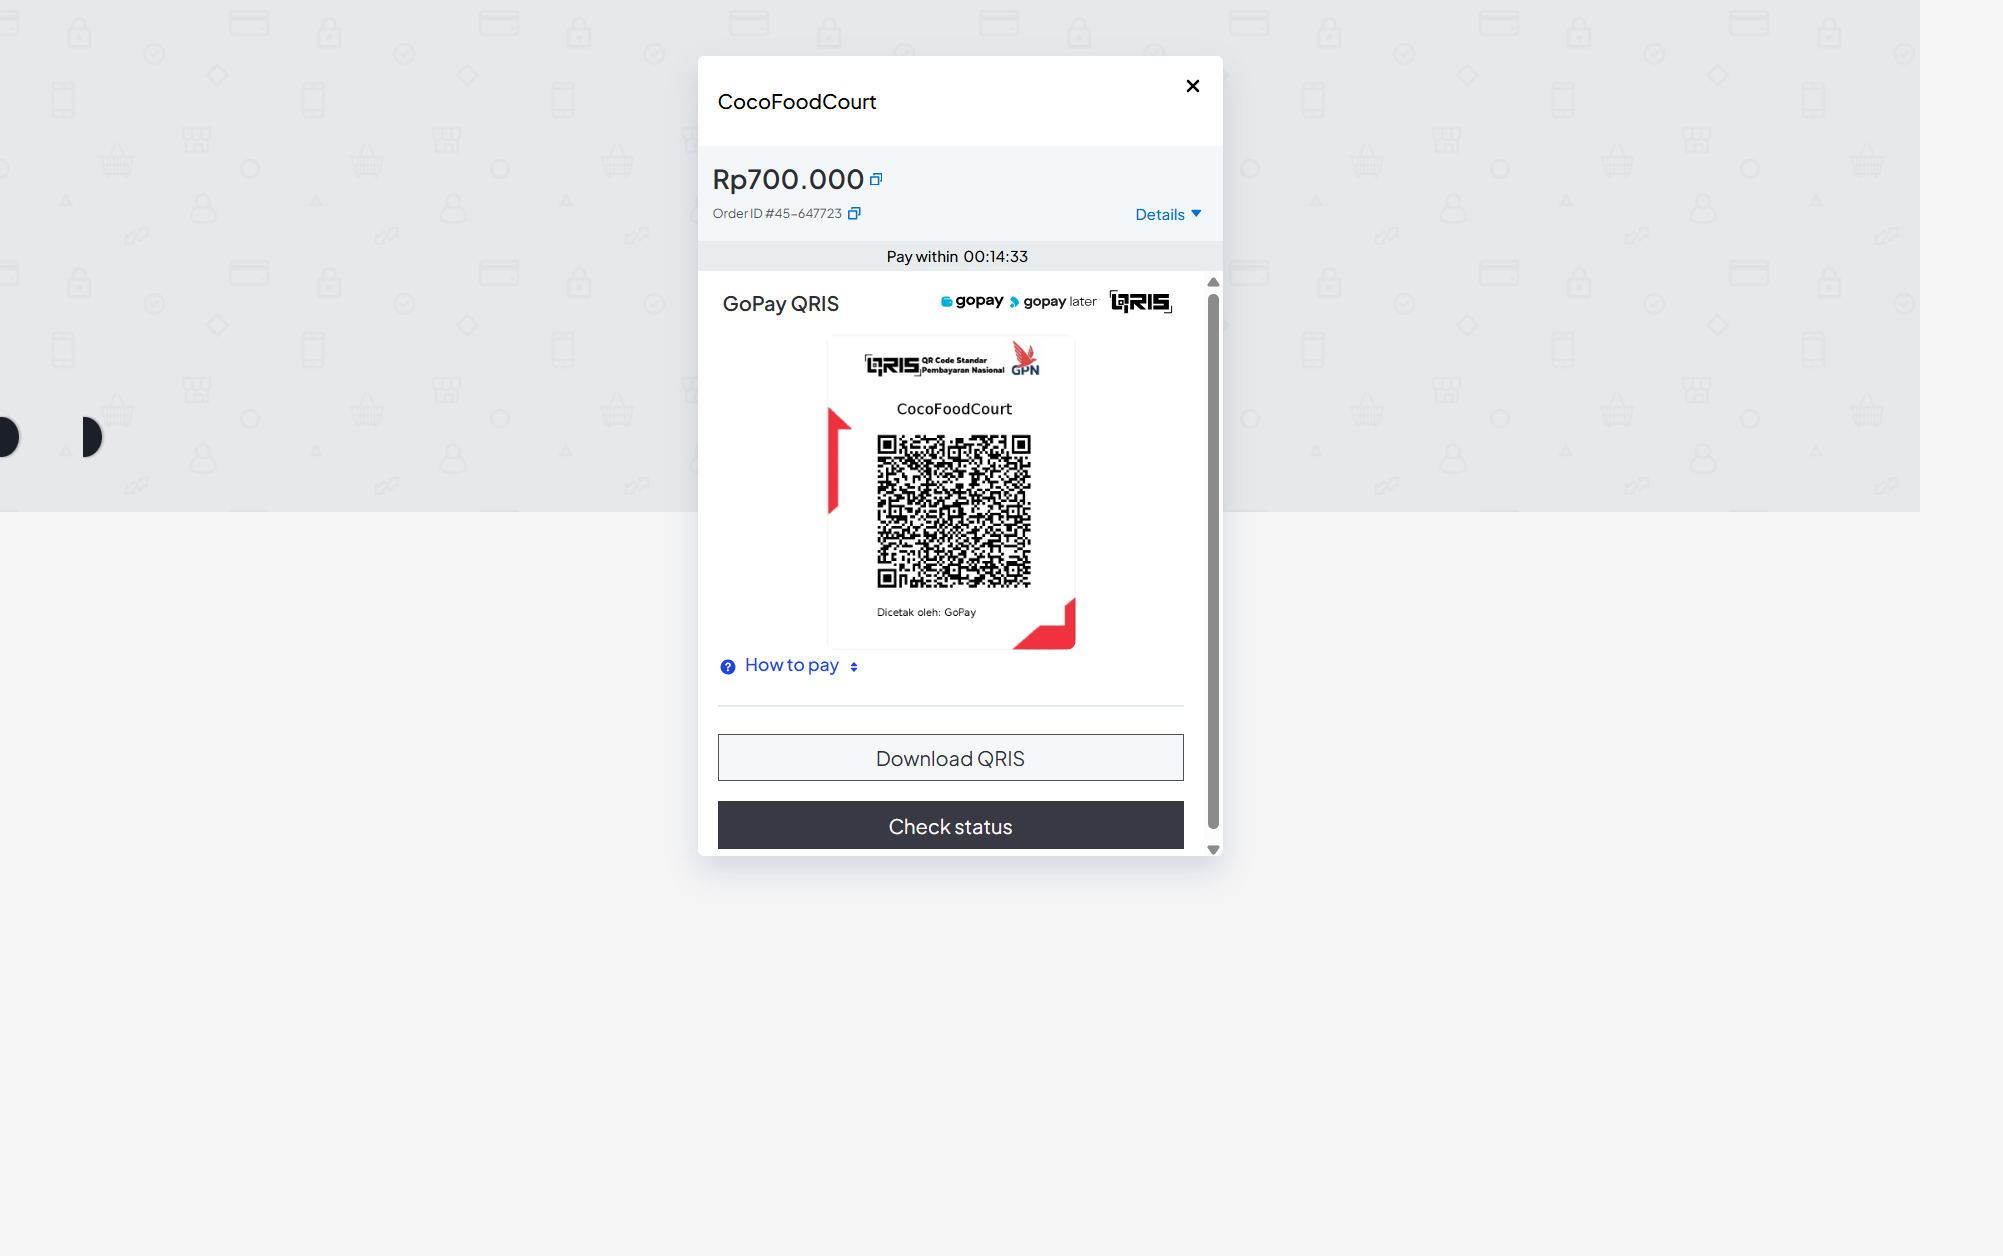
\includegraphics[width=1.0\linewidth]{res/ss_web_step5.png}
    \caption{Tampilan Booking Tahap 5 — Pembayaran via Midtrans}
    \label{fig:ss_step5}
\end{figure}

\textbf{Tahap 6 - Pembayaran Berhasil:}
Setelah proses transaksi selesai, sistem akan menampilkan halaman konfirmasi bahwa pembayaran telah berhasil (\textit{Payment Successful}) beserta nomor pesanan. Pelanggan disediakan tombol untuk kembali melihat daftar reservasi mereka.
\begin{figure}[htbp]
    \centering
    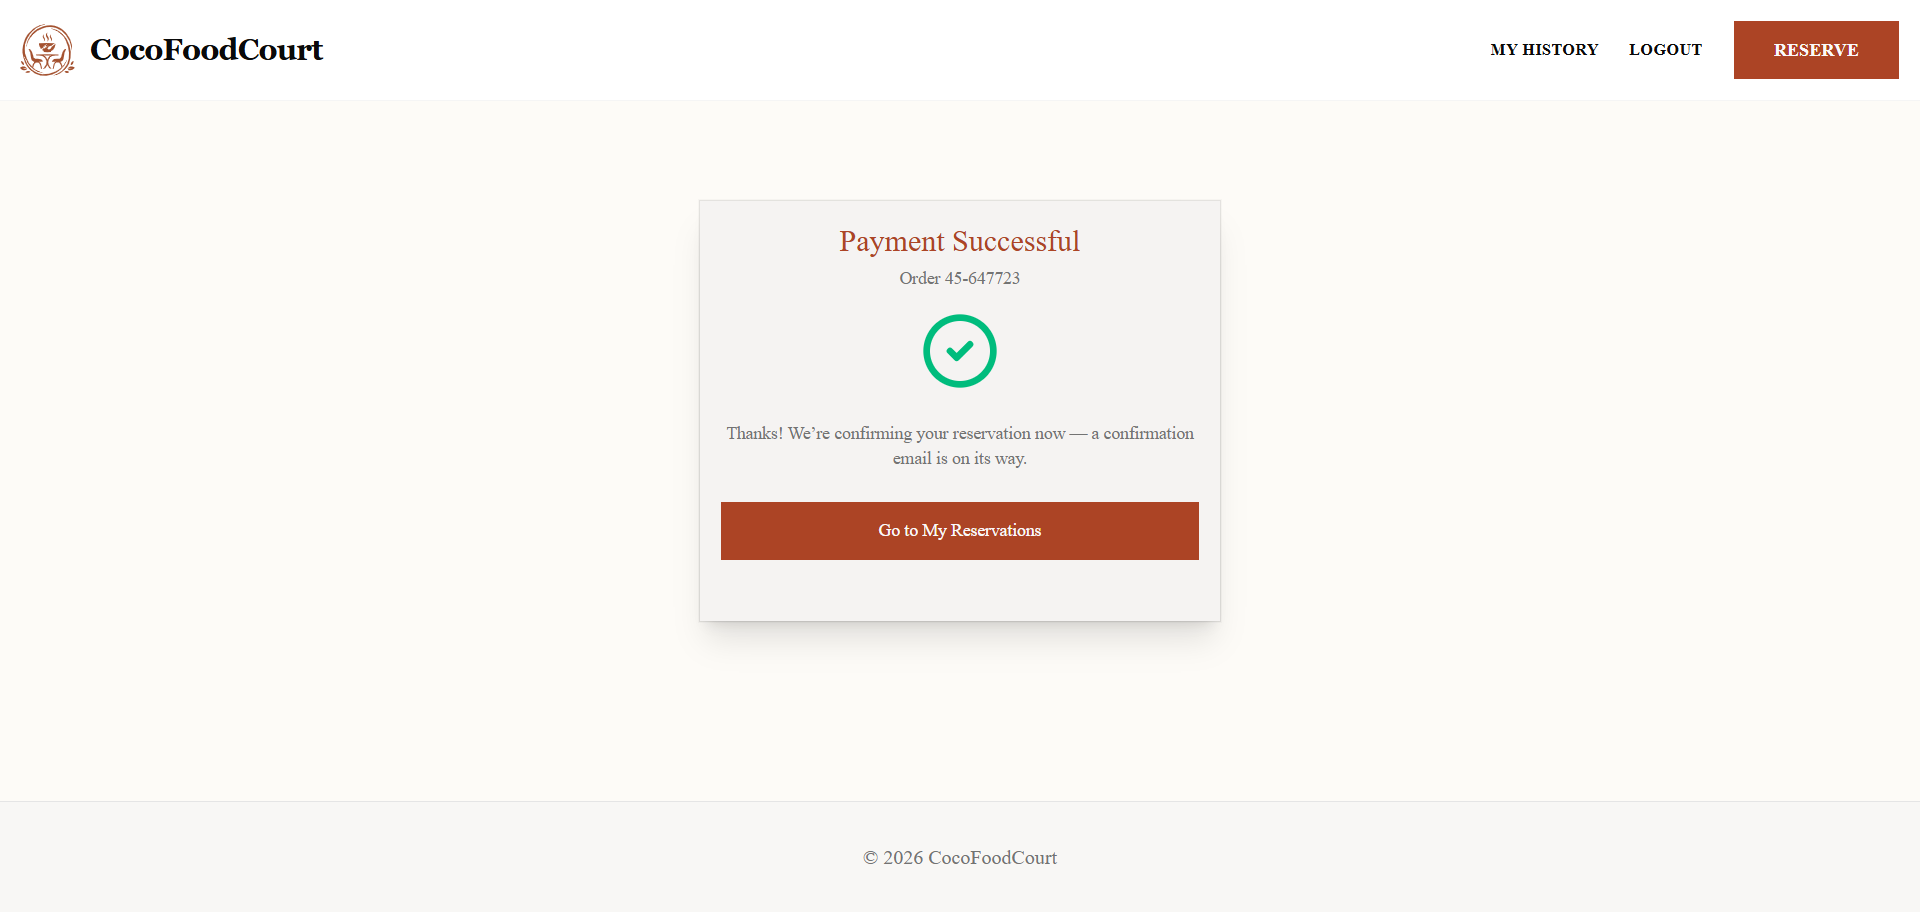
\includegraphics[width=1.0\linewidth]{res/ss_web_step6.png}
    \caption{Tampilan Booking Tahap 6 — Pembayaran Berhasil}
    \label{fig:ss_step6}
\end{figure}

\textbf{Halaman Riwayat Reservasi (Dashboard):}
Halaman \textit{dashboard} menampilkan daftar riwayat dan jadwal reservasi milik pelanggan. Informasi yang disajikan meliputi nomor tiket, tanggal, \textit{time slot}, status reservasi, dan total tagihan \textit{pre-order}. Pelanggan juga dapat membatalkan reservasi melalui halaman ini.
\begin{figure}[htbp]
    \centering
    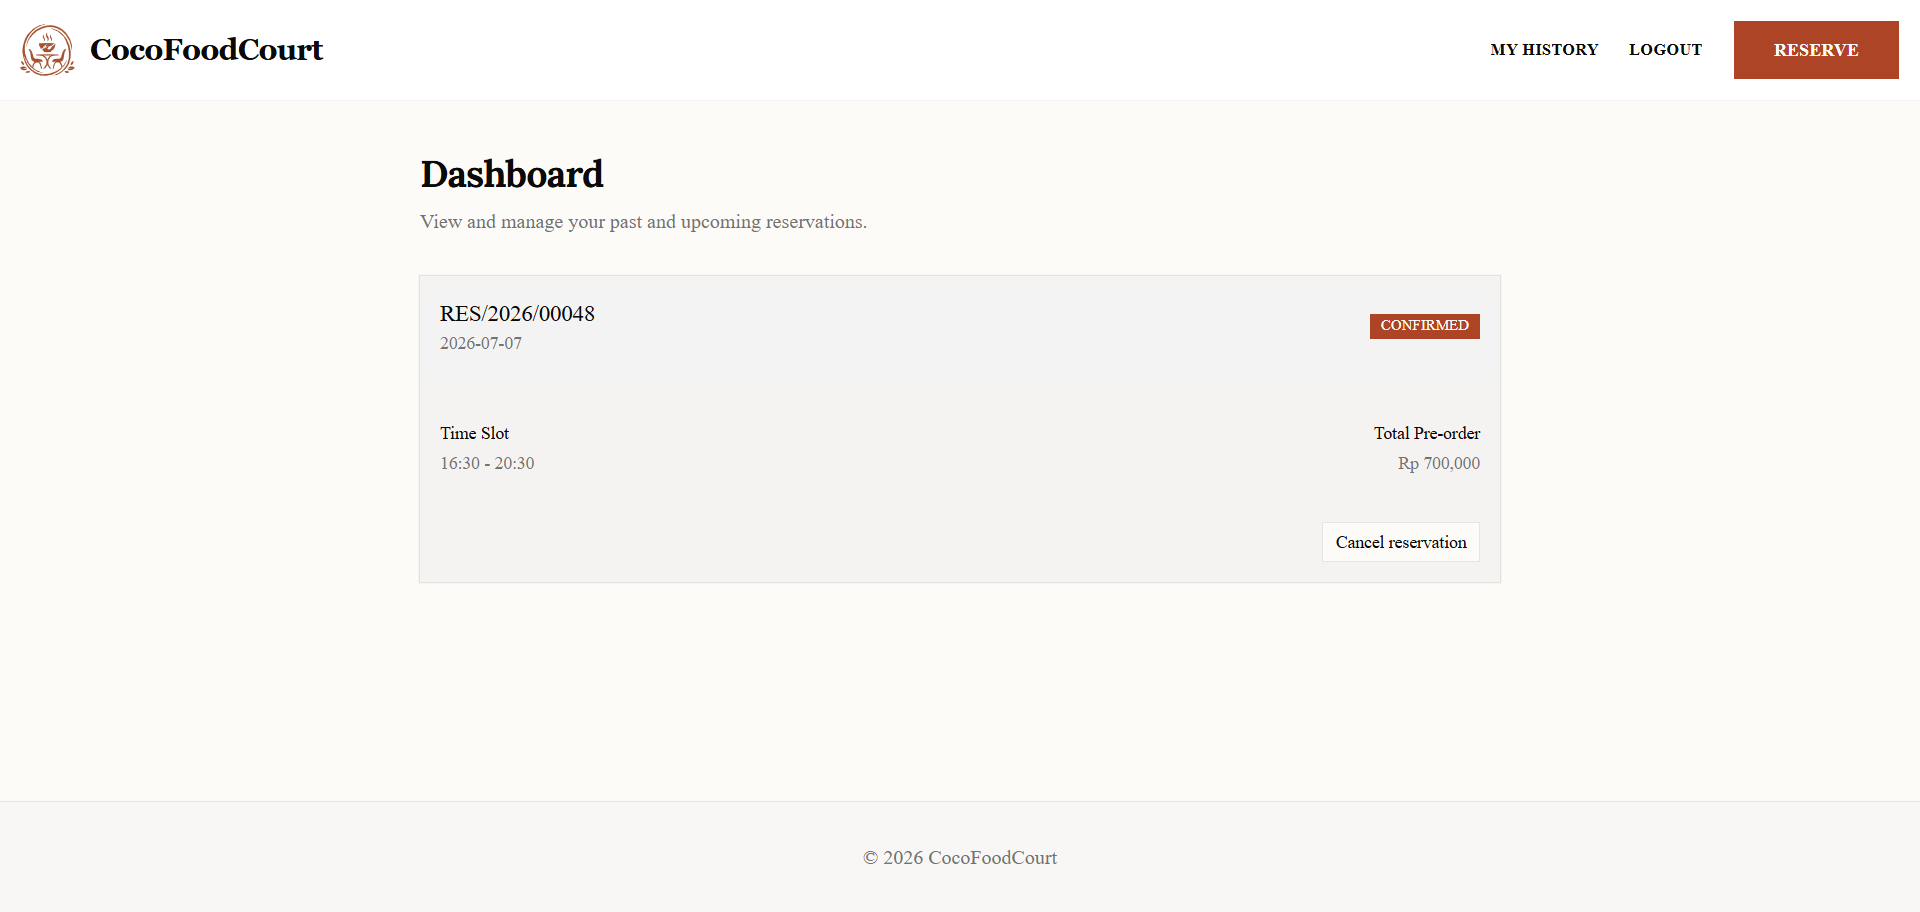
\includegraphics[width=1.0\linewidth]{res/ss_web_history.png}
    \caption{Tampilan Halaman Dashboard — Riwayat Reservasi}
    \label{fig:ss_history}
\end{figure}

\subsubsection{Tampilan Backend Odoo}

\textbf{Daftar Reservasi (List View):}
Admin dapat memantau seluruh reservasi yang masuk melalui tampilan daftar di Odoo. Setiap baris menampilkan nomor referensi, nama pelanggan, tanggal, meja, dan status terkini.
\begin{figure}[htbp]
    \centering
    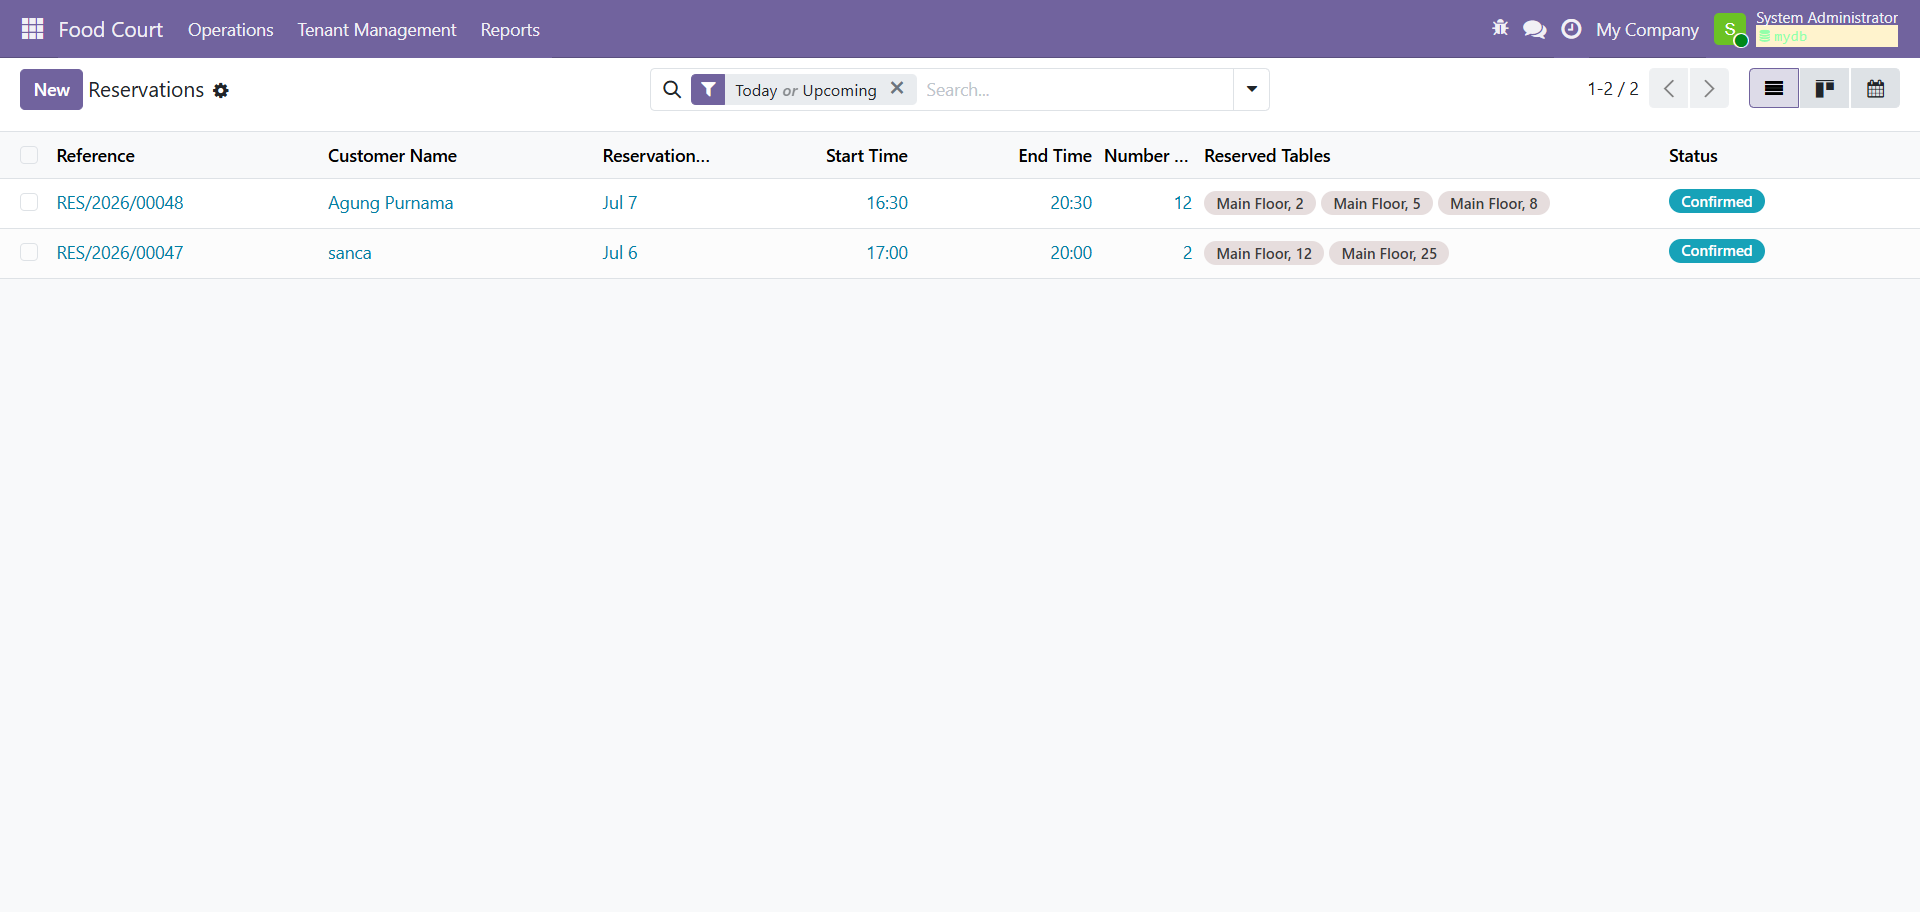
\includegraphics[width=1.0\linewidth]{res/ss_odoo_reservation_list.png}
    \caption{Tampilan Daftar Reservasi di Backend Odoo}
    \label{fig:ss_odoo_list}
\end{figure}

\textbf{Formulir Detail Reservasi:}
Admin dapat melihat dan mengelola detail setiap reservasi, termasuk mengubah status (konfirmasi, \textit{check-in}, selesai, atau batal) langsung melalui tombol aksi di bagian atas formulir.
\begin{figure}[htbp]
    \centering
    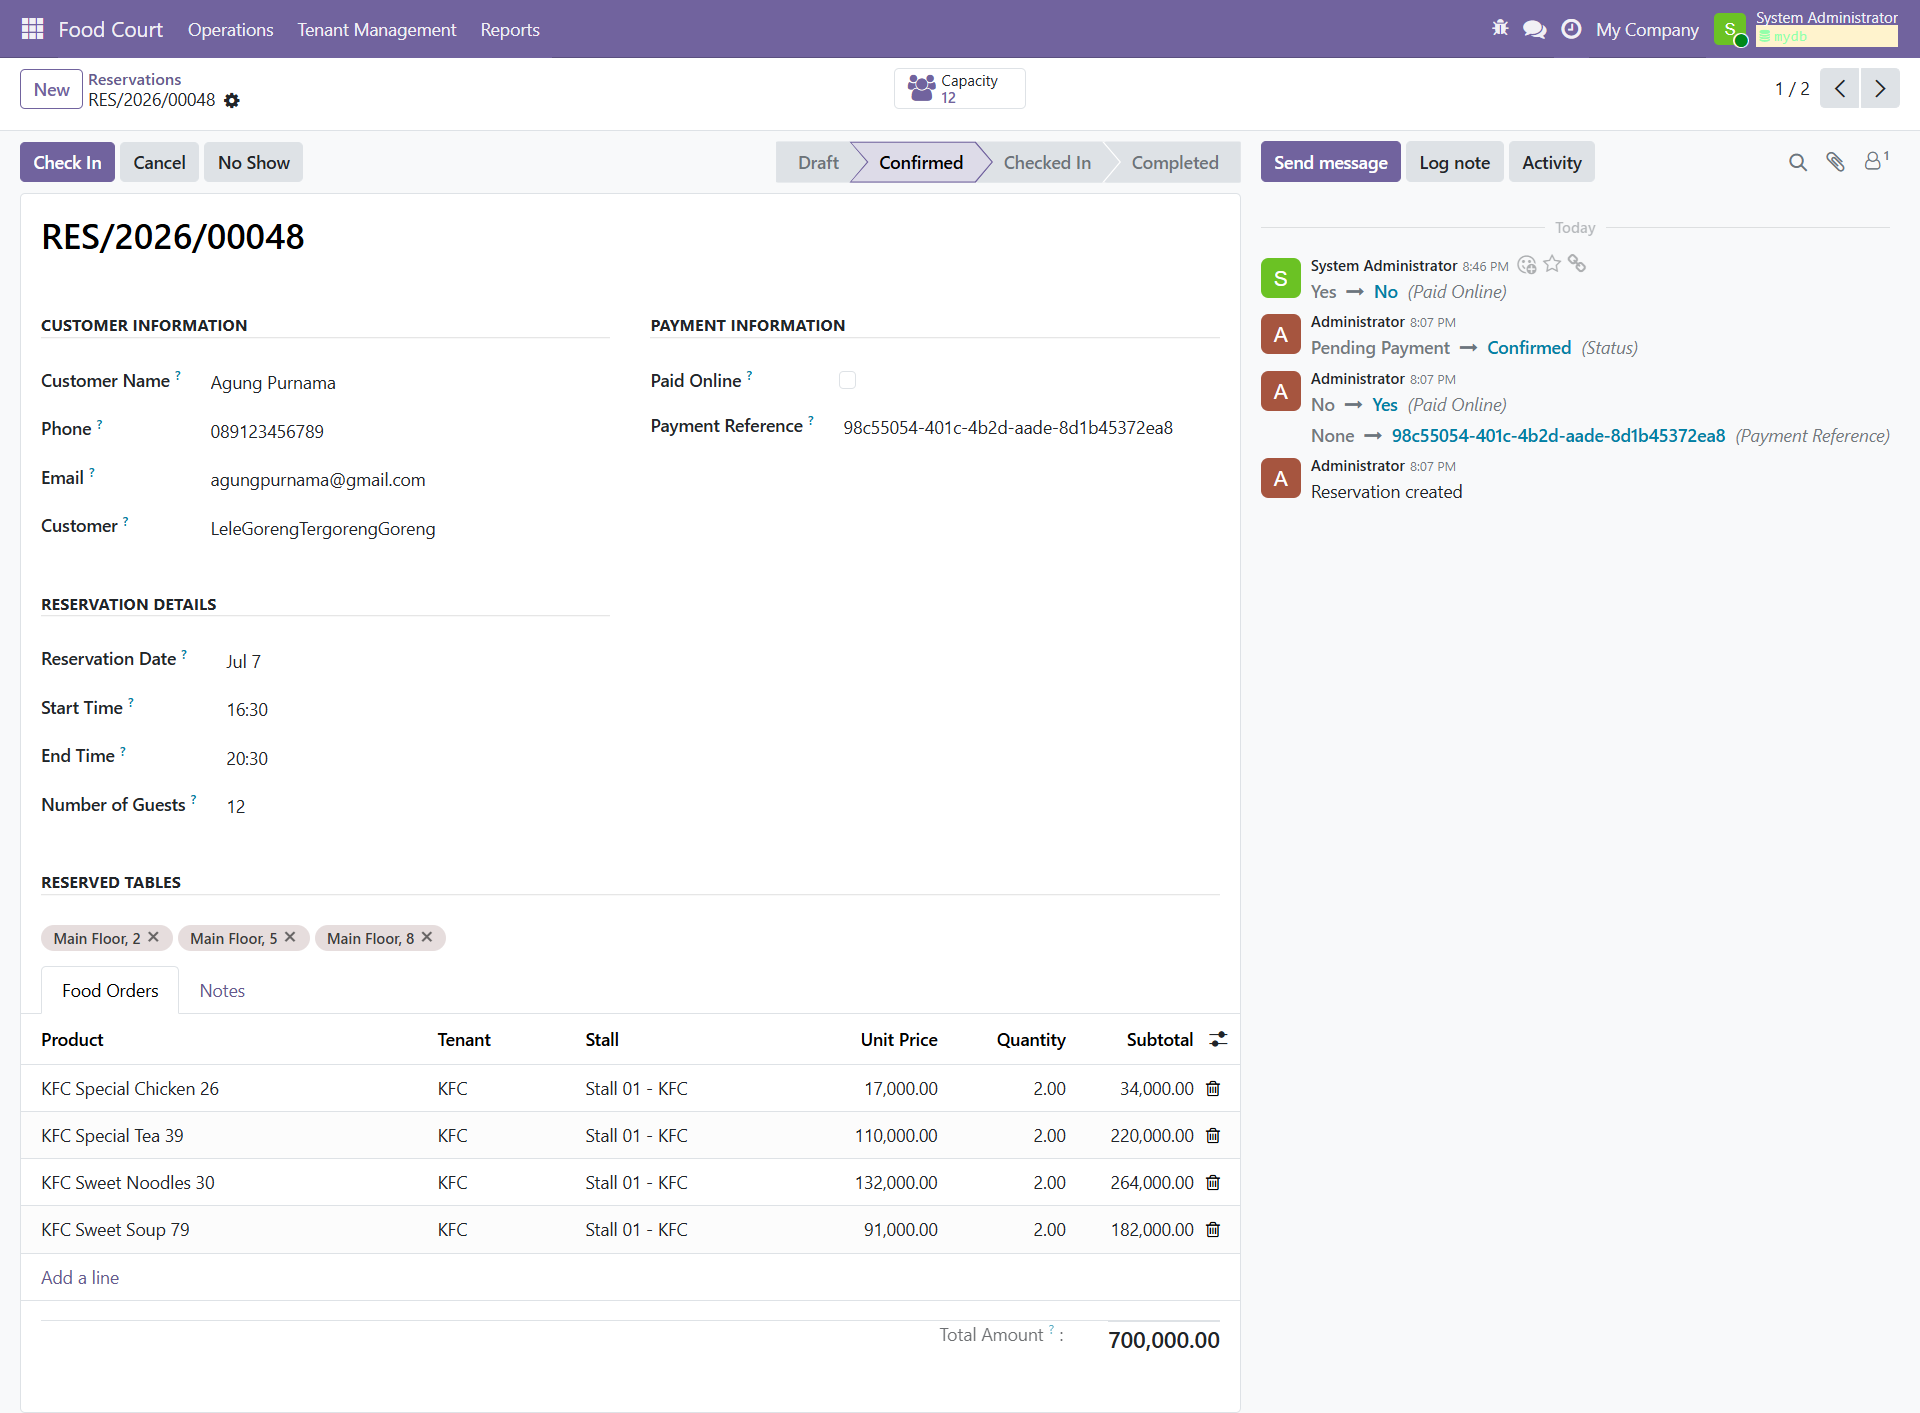
\includegraphics[width=1.0\linewidth]{res/ss_odoo_reservation_form.png}
    \caption{Tampilan Formulir Detail Reservasi di Backend Odoo}
    \label{fig:ss_odoo_form}
\end{figure}

\textbf{Manajemen Tenant:}
Admin dapat mengelola data seluruh tenant yang aktif beroperasi di \textit{food court}, termasuk informasi kontrak, jenis masakan, dan melihat performa penjualan masing-masing tenant secara langsung.
\begin{figure}[htbp]
    \centering
    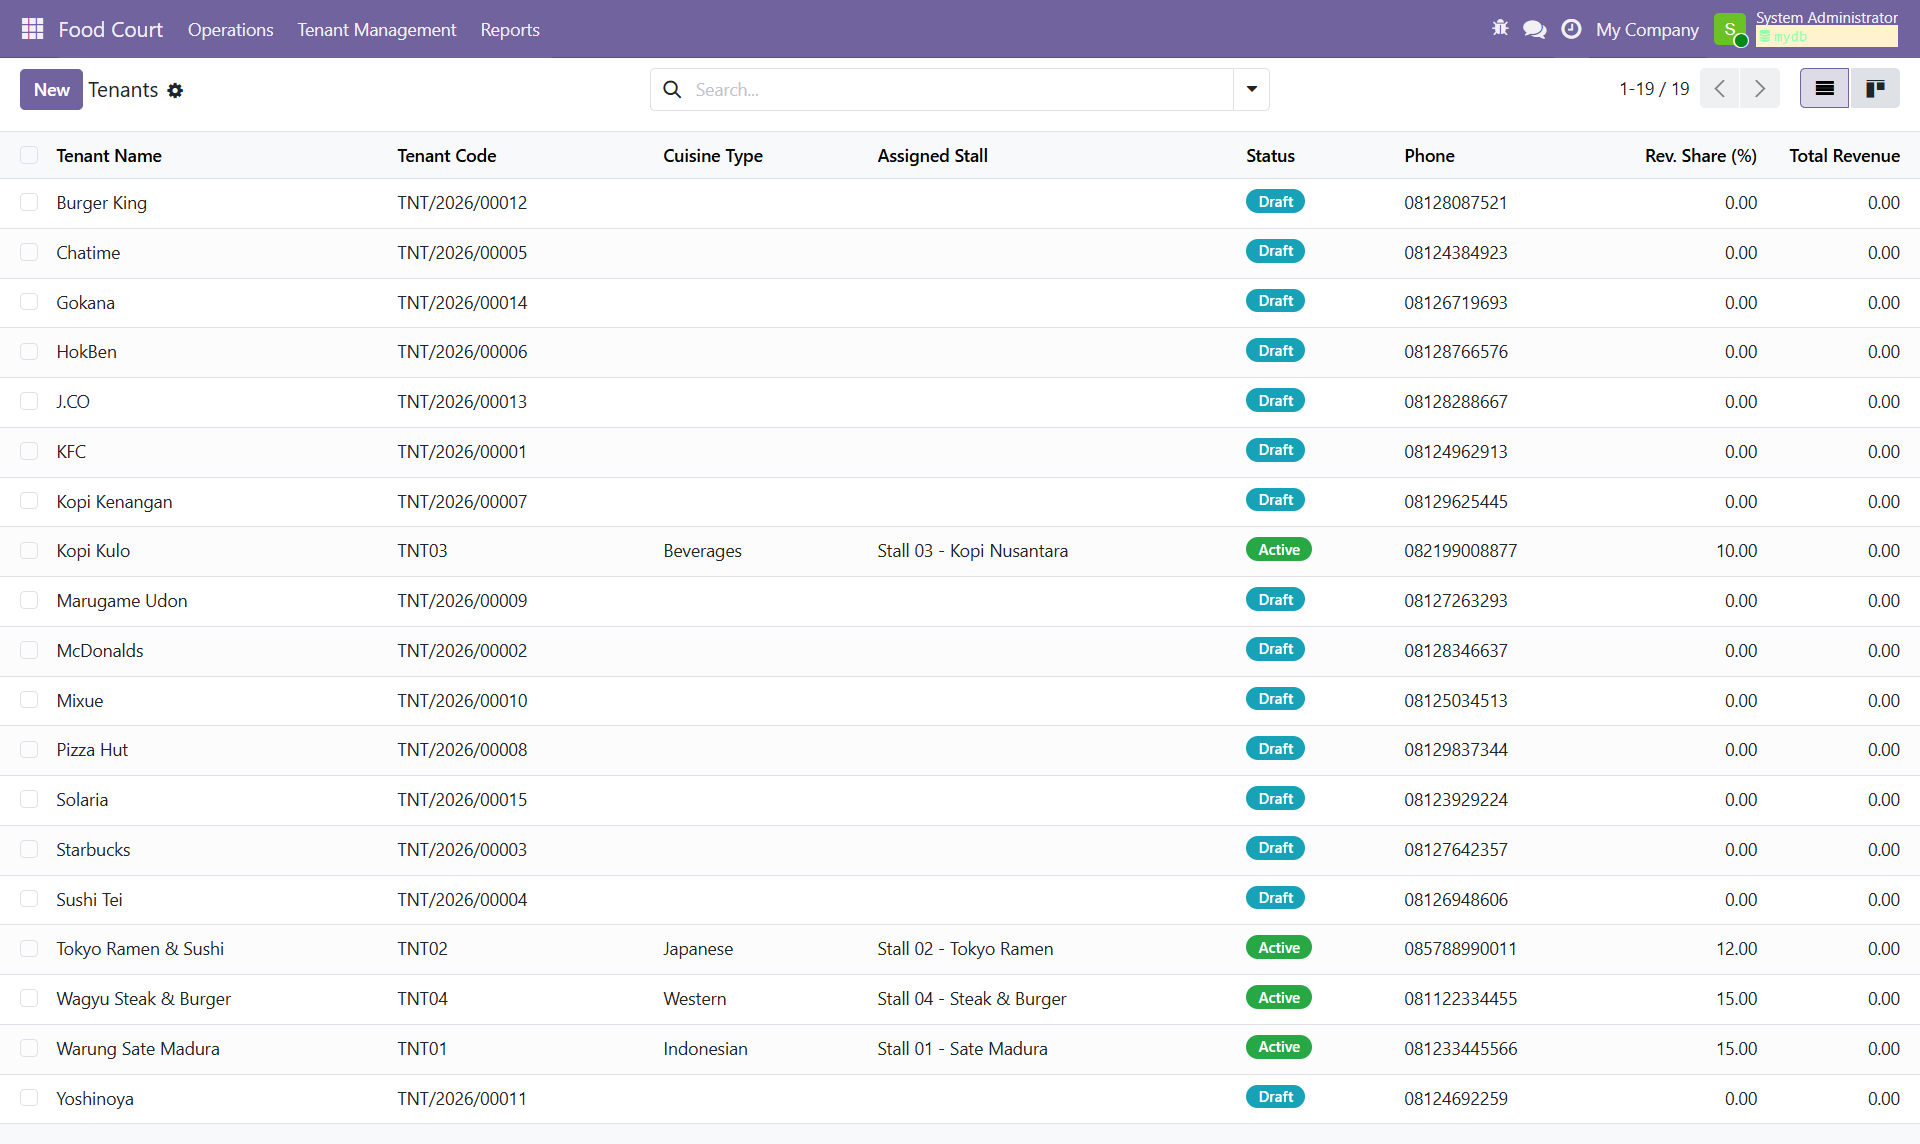
\includegraphics[width=1.0\linewidth]{res/ss_odoo_tenant.png}
    \caption{Tampilan Manajemen Tenant di Backend Odoo}
    \label{fig:ss_odoo_tenant}
\end{figure}

\paragraph{Dasbor Laporan dan Analitik} \mbox{}\\ % \mbox{}\\ digunakan agar teks selanjutnya turun ke baris baru
Odoo menyediakan modul analitik komprehensif yang memungkinkan manajemen untuk mengevaluasi performa operasional \textit{food court} secara *real-time*.

\textbf{Analitik Pendapatan Tenant:}
Tampilan ini menyajikan grafik batang yang membandingkan total pendapatan (termasuk pajak) dari masing-masing tenant yang beroperasi. Data ini memudahkan admin untuk melihat secara langsung tenant mana yang menghasilkan pendapatan tertinggi pada sistem.
\begin{figure}[htbp]
\centering
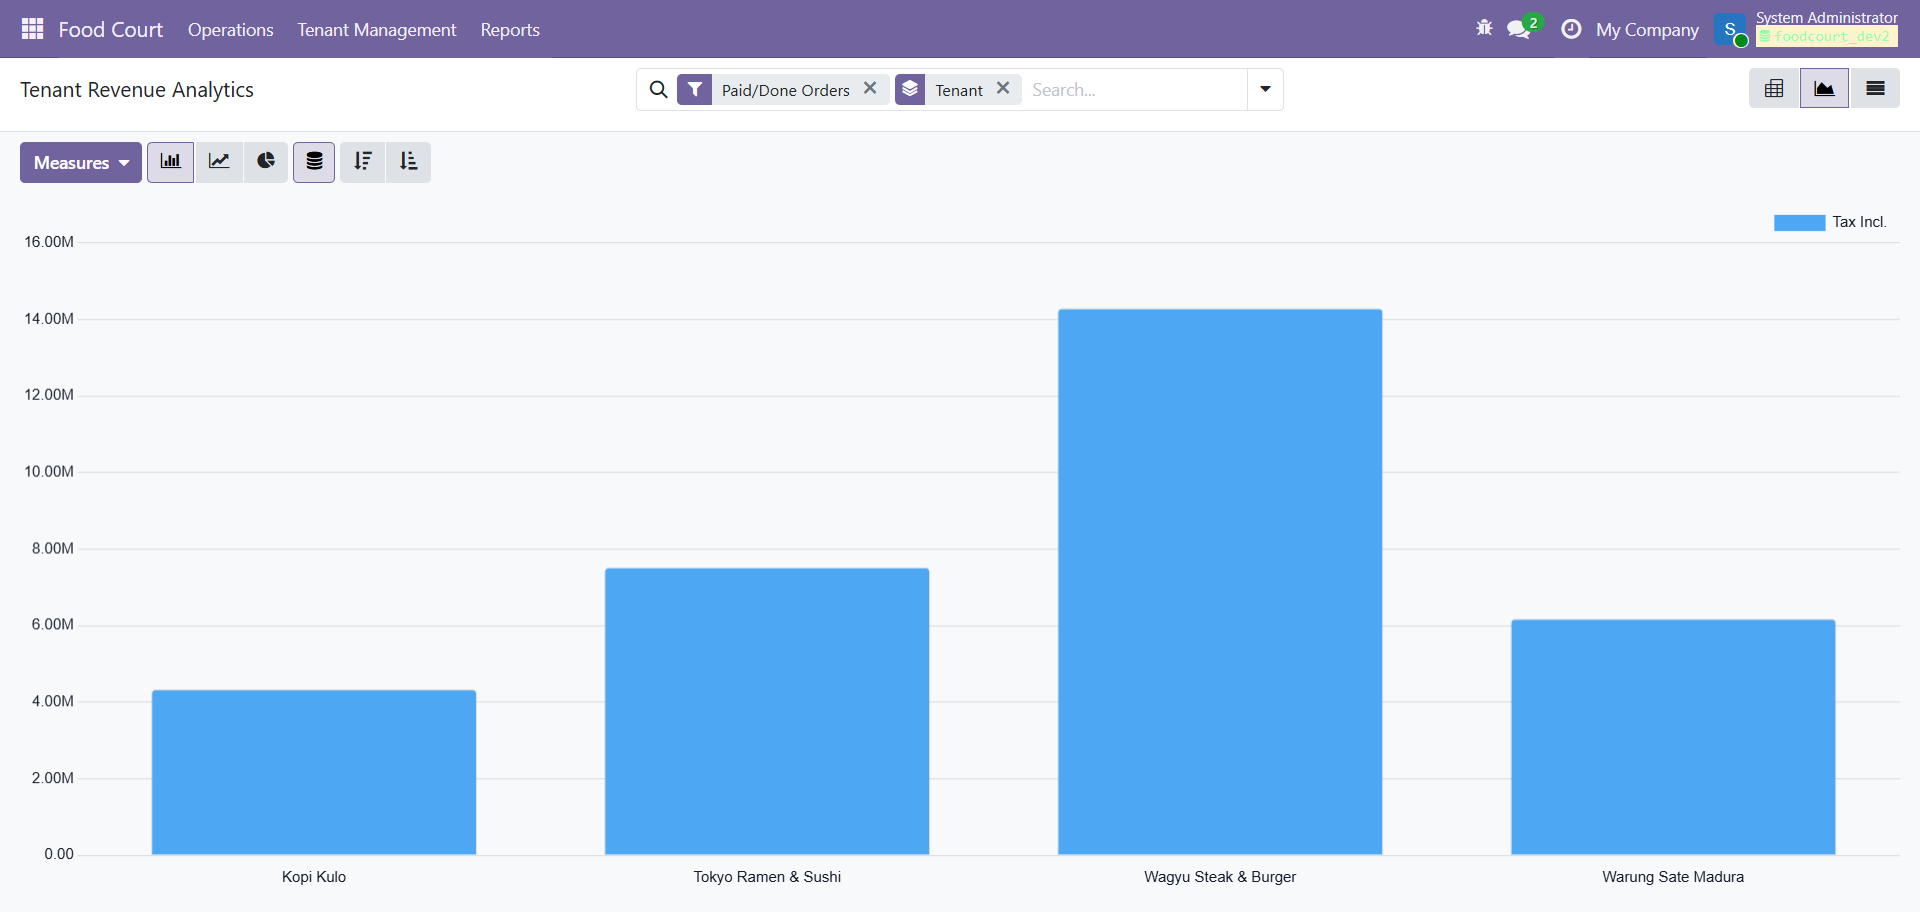
\includegraphics[width=1.0\linewidth]{res/analytics_tenant revenue.png}
\caption{Tampilan Analitik Pendapatan Tenant di Backend Odoo}
\label{fig:analytics_revenue_2}
\end{figure}

\textbf{Kontribusi Penjualan Tenant:}
Grafik lingkaran (\textit{pie chart}) ini memvisualisasikan persentase kontribusi jumlah pesanan dari setiap tenant terhadap keseluruhan transaksi. Tampilan interaktif ini memudahkan admin untuk mengevaluasi pangsa pasar dan performa persentase masing-masing tenant di \textit{food court}.
\begin{figure}[htbp]
\centering
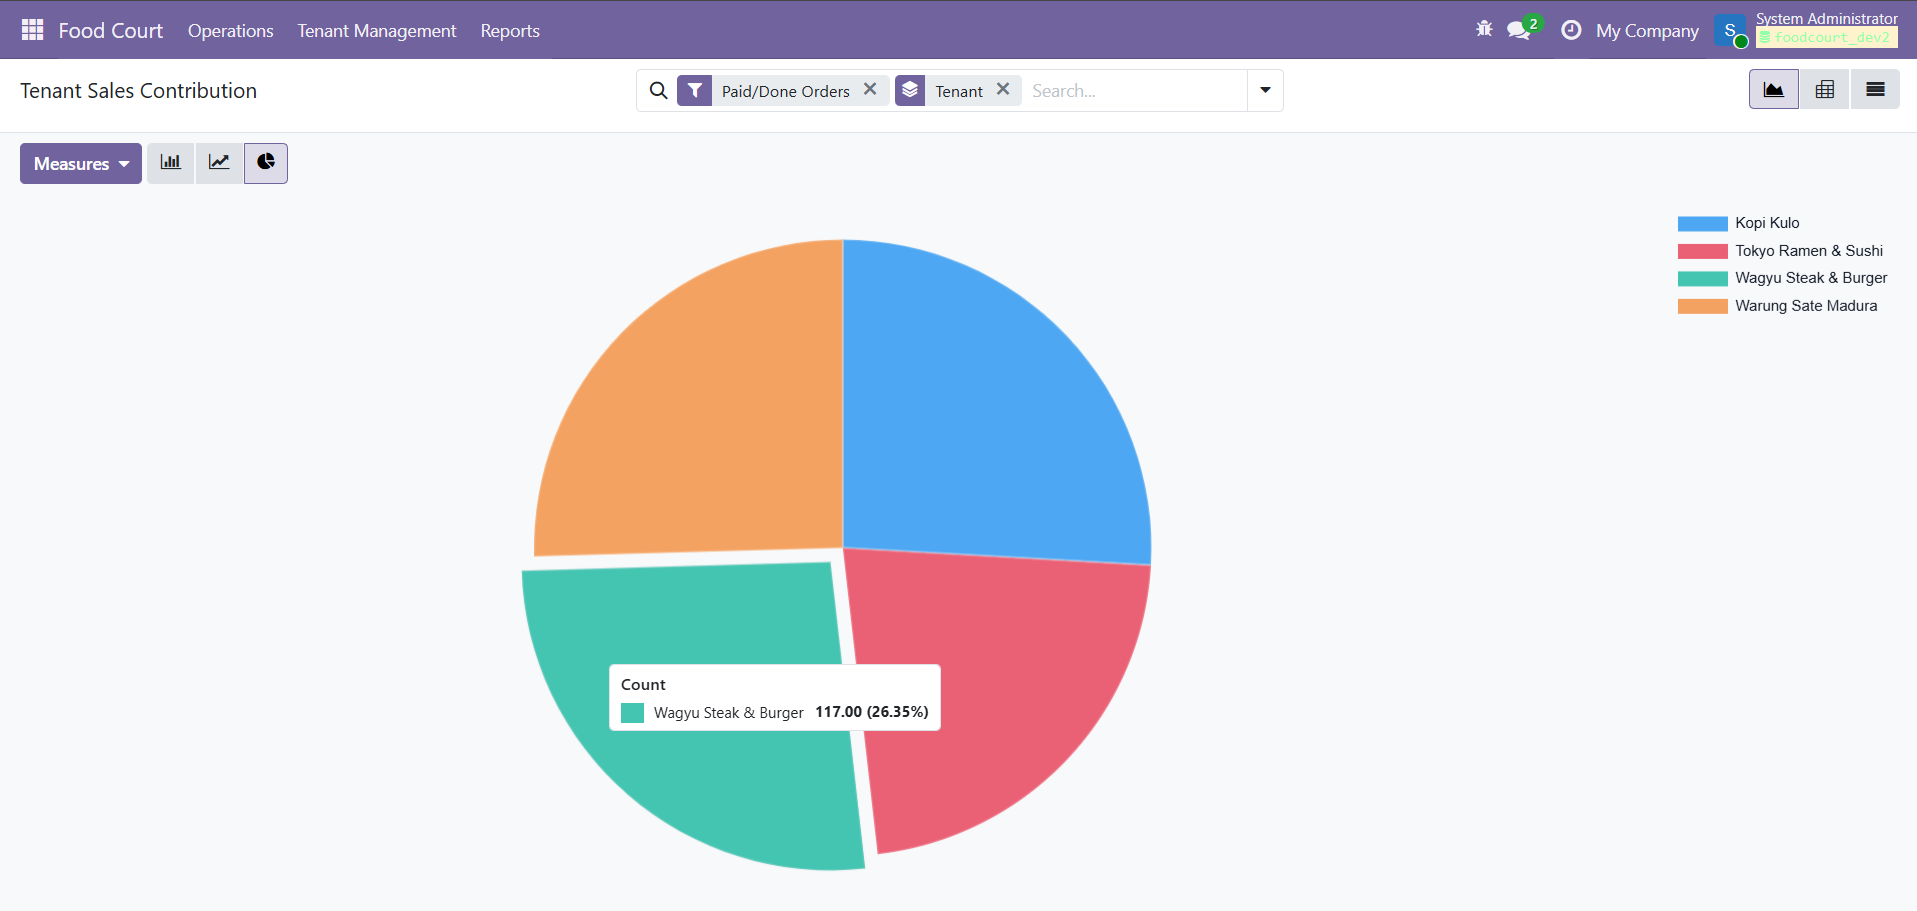
\includegraphics[width=1.0\linewidth]{res/analytics_tenant sales contribution.png}
\caption{Tampilan Pie Chart Kontribusi Penjualan Tenant di Backend Odoo}
\label{fig:analytics_contribution_pie}
\end{figure}

\textbf{Analitik Jumlah Tamu (Number of Guests):}
Laporan ini menggunakan grafik batang untuk menampilkan fluktuasi total jumlah tamu yang hadir berdasarkan data reservasi harian. Informasi ini sangat berguna bagi manajemen untuk memperkirakan volume pengunjung dan menyesuaikan kebutuhan staf pelayanan di lapangan.
\begin{figure}[htbp]
\centering
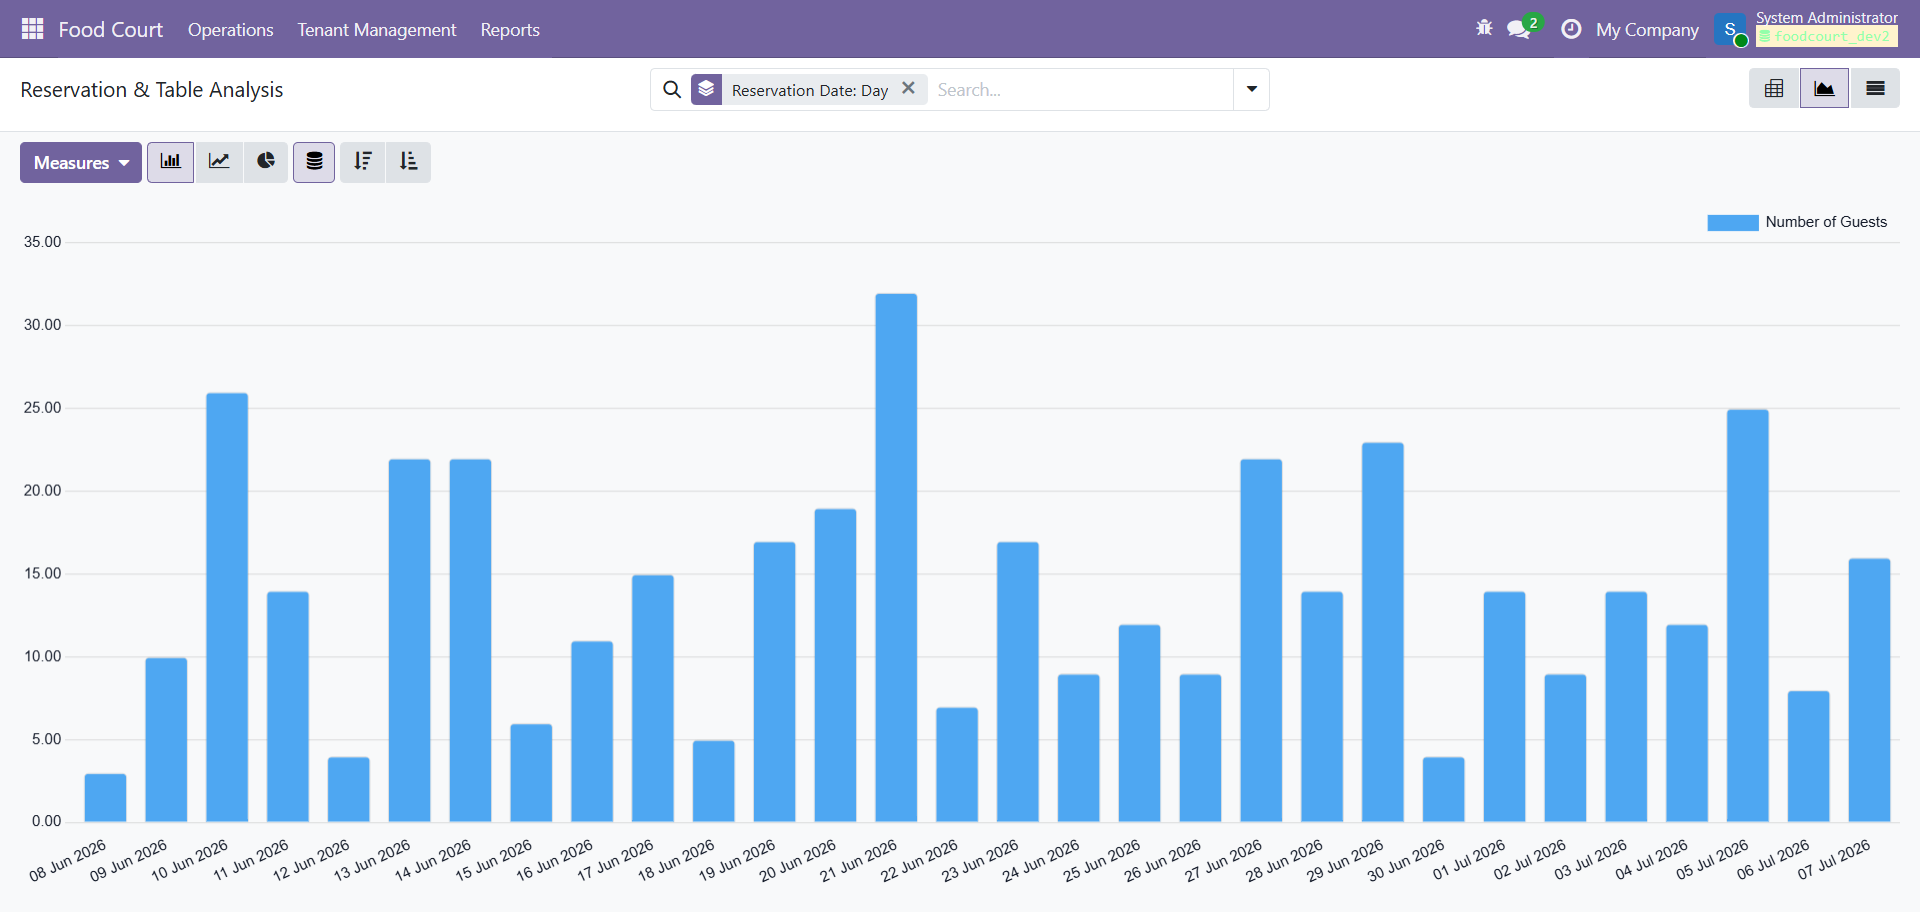
\includegraphics[width=1.0\linewidth]{res/analytics_number of guests.png}
\caption{Tampilan Analitik Jumlah Tamu Harian di Backend Odoo}
\label{fig:analytics_guests}
\end{figure}

\textbf{Tren Reservasi Harian:}
Admin dapat memantau tren jumlah reservasi aktif dari hari ke hari melalui grafik area (\textit{area chart}). Tampilan ini membantu manajemen dalam mengenali pola kunjungan, melihat puncak keramaian pada tanggal tertentu, dan mengevaluasi efektivitas layanan.
\begin{figure}[htbp]
\centering
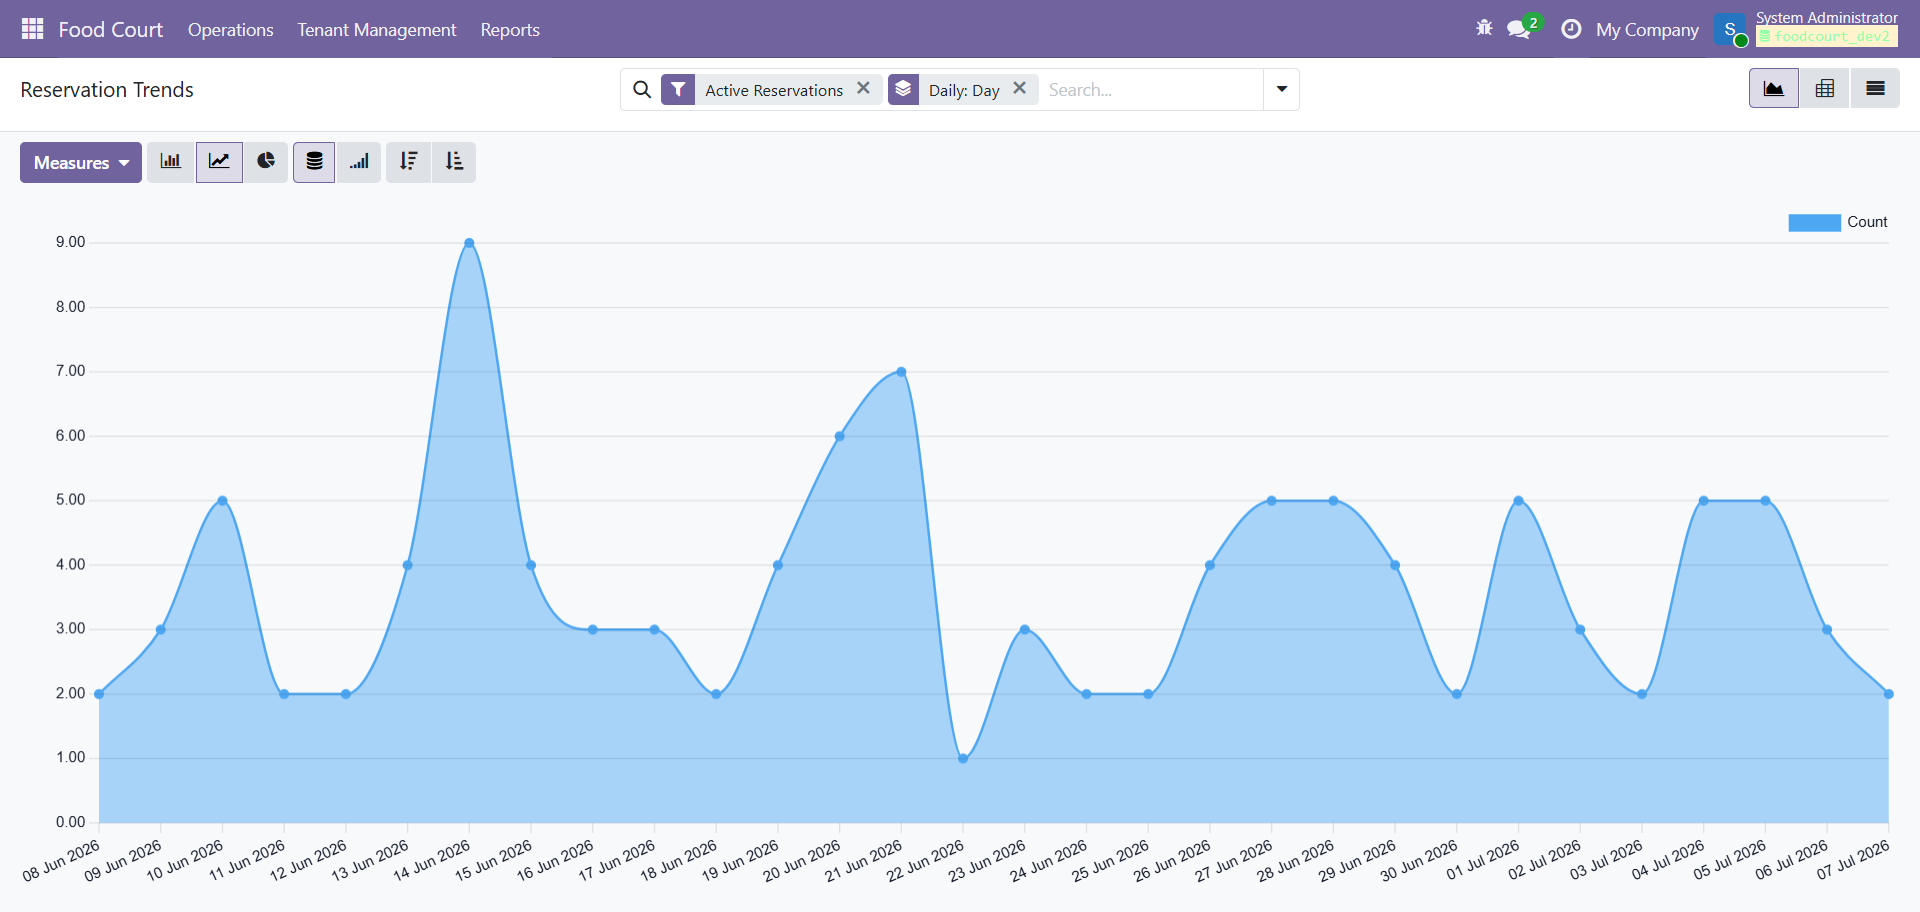
\includegraphics[width=1.0\linewidth]{res/analytics_reservation trends.png}
\caption{Tampilan Tren Reservasi Harian di Backend Odoo}
\label{fig:analytics_trends_2}
\end{figure}

\textbf{Analitik Okupansi Meja:}
Tampilan ini menggunakan grafik batang bertumpuk (\textit{stacked bar chart}) yang dipadukan dengan grafik garis untuk menganalisis tingkat okupansi meja berdasarkan jam operasional dan hari dalam seminggu. Hal ini memudahkan penentuan waktu sibuk (\textit{peak hours}) secara komprehensif.
\begin{figure}[htbp]
\centering
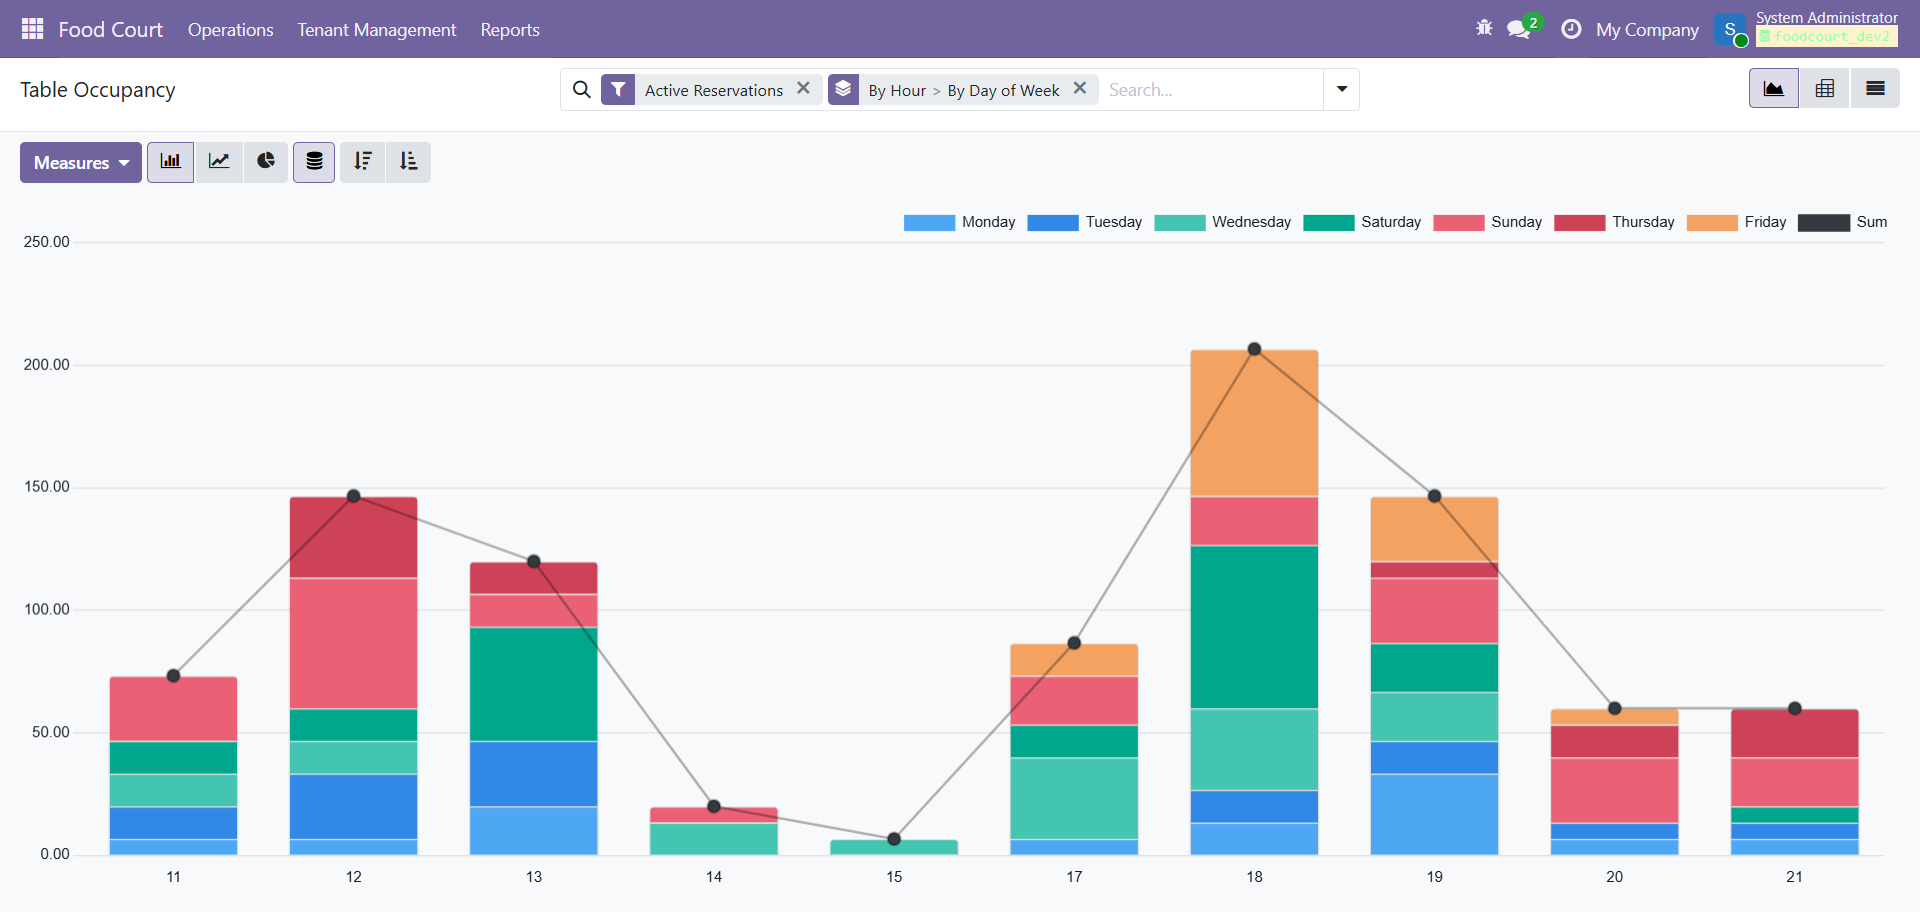
\includegraphics[width=1.0\linewidth]{res/analytics_table occupancy.png}
\caption{Tampilan Analitik Okupansi Meja di Backend Odoo}
\label{fig:analytics_occupancy_2}
\end{figure}

\section{PENGUJIAN SISTEM}

Pengujian sistem dilakukan menggunakan metode \textit{Black-Box Testing}, yaitu pengujian yang berfokus pada fungsionalitas sistem dari sudut pandang pengguna tanpa memperhatikan struktur kode internal. Pendekatan ini dipilih karena sesuai dengan tujuan verifikasi, yakni memastikan bahwa keluaran sistem sesuai dengan kebutuhan fungsional yang telah didefinisikan pada tahap analisis, terlepas dari bagaimana implementasi kode di dalamnya dilakukan.

\subsection{Skenario dan Hasil Pengujian}
Skenario pengujian difokuskan pada alur bisnis inti sistem, mulai dari proses pemesanan oleh pelanggan di sisi \textit{Web Frontend} hingga penyelesaian reservasi dan proses otomatis di sisi \textit{Backend} Odoo. Setiap skenario mewakili satu fungsi kritis yang apabila gagal akan berdampak langsung pada keberjalanan proses bisnis. Kolom \textit{Hasil Pengujian} pada tabel berikut merupakan keluaran aktual yang diamati saat skenario dieksekusi.

\begin{table*}[htbp]
\caption{Skenario dan Hasil Pengujian Sistem Reservasi Food Court}
\label{tab:test_scenarios}
\centering
\footnotesize
\begin{tabularx}{\textwidth}{|
>{\centering\arraybackslash}p{0.7cm}|
>{\raggedright\arraybackslash}p{2.4cm}|
>{\raggedright\arraybackslash}p{2.5cm}|
>{\raggedright\arraybackslash}X|
>{\raggedright\arraybackslash}X|
>{\centering\arraybackslash}p{1.2cm}|}
\hline
\textbf{ID} & \textbf{Skenario} & \textbf{Prasyarat} & \textbf{Hasil yang Diharapkan} & \textbf{Hasil Pengujian} & \textbf{Status} \\
\hline
TC01 & Pencarian meja berdasarkan waktu & Server Next.js dan Odoo aktif, data meja tersedia & Sistem menampilkan denah lantai dengan meja yang berstatus tersedia sesuai parameter waktu yang dipilih & Denah lantai berhasil ditampilkan; meja yang sudah direservasi pada slot waktu tersebut ditandai berbeda dengan warna redup & Sukses \\
\hline
TC02 & Pemilihan meja pada denah interaktif & Halaman booking berada di Tahap 2 & Meja yang diklik berubah tampilan menjadi terpilih, dan informasi kapasitas kursi diperbarui & Meja berubah warna menjadi warna aksen terpilih; panel informasi di bawah peta menampilkan kapasitas meja dan perbandingan terhadap jumlah tamu & Sukses \\
\hline
TC03 & Penambahan menu \textit{pre-order} & Halaman booking berada di Tahap 3, menu tersedia & Kuantitas item bertambah, total harga \textit{pre-order} diperbarui secara langsung & Kuantitas item bertambah setiap kali tombol ``+'' ditekan; panel total di bagian bawah halaman langsung memperbarui nominal tanpa \textit{reload} & Sukses \\
\hline
TC04 & Pengiriman reservasi oleh pelanggan terdaftar & Pelanggan sudah \textit{login}, berada di Tahap 4 & Reservasi berhasil tersimpan di Odoo, pelanggan diarahkan ke halaman \textit{dashboard} riwayat & Rekaman reservasi baru muncul di Odoo dengan status \textit{Draft}; pelanggan diarahkan ke halaman \texttt{/dashboard} yang menampilkan reservasi baru tersebut & Sukses \\
\hline
TC05 & Konfirmasi reservasi oleh admin & Reservasi berstatus \textit{Draft} tersedia di Odoo & Status reservasi berubah menjadi \textit{Confirmed}, status meja terkait berubah menjadi \textit{Reserved} & Status berubah sesuai harapan; e-mail konfirmasi terkirim otomatis ke alamat pelanggan; tombol ``Confirm'' berubah menjadi tidak aktif setelah diklik & Sukses \\
\hline
TC06 & Proses \textit{check-in} tamu & Reservasi berstatus \textit{Confirmed} & Status berubah menjadi \textit{Checked In}, meja berubah menjadi \textit{Occupied}, dan pesanan POS otomatis terbuat dari data \textit{pre-order} & Rekaman \texttt{pos.order} baru terbuat secara otomatis dengan baris-baris pesanan sesuai data \textit{pre-order}; status meja berubah menjadi \textit{Occupied} di tampilan denah lantai Odoo & Sukses \\
\hline
TC07 & Penyelesaian reservasi & Reservasi berstatus \textit{Checked In} & Status reservasi berubah menjadi \textit{Completed}, meja kembali berstatus \textit{Available} & Status berubah menjadi \textit{Completed}; meja kembali berstatus \textit{Available} sehingga dapat dipilih kembali pada reservasi berikutnya & Sukses \\
\hline
TC08 & Pencegahan pemesanan ganda (\textit{double booking}) & Meja A sudah direservasi pada rentang jam 12:00–13:00 & Sistem menolak pembuatan reservasi dan menampilkan pesan \textit{error} bahwa meja sudah terpesan & Odoo mengembalikan \textit{ValidationError}; pesan \textit{error} diteruskan ke antarmuka Next.js dan ditampilkan kepada pengguna; reservasi baru tidak tersimpan & Sukses \\
\hline
TC09 & Pembayaran \textit{pre-order} via Midtrans & Reservasi dengan item \textit{pre-order} berhasil dibuat & Midtrans mengirimkan notifikasi \textit{webhook}, status reservasi di Odoo diperbarui menjadi \textit{Confirmed} secara otomatis & Halaman Midtrans Snap terbuka dengan nominal yang sesuai; setelah pembayaran diselesaikan menggunakan kartu uji coba, \textit{webhook} diterima dan status reservasi di Odoo berubah menjadi \textit{Confirmed} tanpa intervensi manual & Sukses \\
\hline
TC10 & Pembatalan otomatis pembayaran kadaluarsa & Reservasi berstatus \textit{Pending Payment} sudah ada lebih dari 15 menit & Status reservasi berubah menjadi \textit{Cancelled}, meja kembali tersedia, dan catatan pembatalan otomatis tercatat di \textit{log} aktivitas & Setelah \textit{cron job} dijalankan secara manual, reservasi yang melewati batas waktu diubah menjadi \textit{Cancelled}; meja kembali tersedia; \textit{log} aktivitas mencatat pesan ``Otomatis dibatalkan karena pembayaran tidak diselesaikan'' & Sukses \\
\hline
\end{tabularx}
\end{table*}

\subsection{Analisis Hasil Pengujian}
Berdasarkan eksekusi seluruh skenario pada Tabel~\ref{tab:test_scenarios}, semua sepuluh skenario (TC01–TC10) menghasilkan output yang sesuai dengan yang diharapkan, sehingga tingkat keberhasilan pengujian mencapai \textbf{100\%} (10 dari 10 skenario berhasil).

Beberapa temuan spesifik yang diperoleh selama pengujian diuraikan sebagai berikut:

\textbf{Alur Pemesanan Frontend (TC01–TC04).}
Keseluruhan alur pemesanan empat tahap berjalan secara mulus tanpa gangguan. Mekanisme \textit{state persistence} berbasis \texttt{localStorage} terbukti berfungsi dengan baik: data formulir yang telah diisi pada tahap sebelumnya tetap tersimpan ketika pengguna berpindah antar tahap, sehingga tidak ada data yang hilang. Pada TC03, pembaruan total harga \textit{pre-order} berlangsung secara \textit{real-time} tanpa perlu memuat ulang halaman, yang memberikan pengalaman pengguna yang responsif.

\textbf{State Machine Reservasi di Odoo (TC05–TC07).}
Transisi status reservasi berjalan sesuai dengan desain \textit{state machine} yang telah didefinisikan. Pada TC05, selain perubahan status, sistem juga secara otomatis mengirimkan e-mail konfirmasi kepada pelanggan, yang mengonfirmasi bahwa integrasi \textit{mail template} Odoo berfungsi dengan benar. Pada TC06, pembuatan pesanan POS secara otomatis dari data \textit{pre-order} adalah fitur paling kritis dalam integrasi antara modul \texttt{foodcourt} dan modul \texttt{point\_of\_sale}, dan fitur ini terbukti berjalan tanpa \textit{error}.

\textbf{Integritas Data dan Validasi Bisnis (TC08).}
Mekanisme pencegahan \textit{double booking} yang diimplementasikan melalui metode \texttt{\_check\_table\_availability()} berhasil menolak seluruh percobaan pembuatan reservasi yang bertumpang-tindih. Pesan galat yang dikembalikan oleh Odoo berhasil diteruskan dan ditampilkan di antarmuka pengguna, sehingga pengguna mendapatkan informasi yang jelas mengenai penyebab kegagalan.

\textbf{Integrasi Pihak Ketiga dan Proses Otomatis (TC09–TC10).}
Alur pembayaran \textit{end-to-end} melalui Midtrans Snap (TC09) berjalan sesuai desain. Notifikasi \textit{webhook} dari Midtrans berhasil diterima oleh \textit{endpoint} \texttt{/api/webhooks} dan memperbarui status reservasi di Odoo tanpa memerlukan tindakan manual dari admin, yang mengkonfirmasi keandalan arsitektur integrasi pihak ketiga. Pada TC10, \textit{cron job} pembatalan otomatis berhasil mengidentifikasi dan membatalkan reservasi yang melewati batas waktu pembayaran, serta membebaskan slot meja yang sebelumnya terkunci, sehingga mencegah terjadinya \textit{resource lock} yang dapat menghambat operasional sistem.

\section{KESIMPULAN DAN SARAN}

\subsection{Kesimpulan}
Berdasarkan keseluruhan proses analisis, perancangan, implementasi, dan pengujian yang telah dilakukan, dapat ditarik beberapa kesimpulan sebagai berikut:

\begin{enumerate}
    \item Sistem reservasi terpusat berhasil dibangun dengan mengintegrasikan \textit{Web Frontend} (Next.js) dan \textit{Backend} ERP (Odoo 19) melalui protokol XML-RPC. Pendekatan arsitektur \textit{decoupled} ini memungkinkan pelanggan melakukan reservasi secara mandiri melalui antarmuka web, sementara seluruh data tersimpan dan dikelola secara terpusat di Odoo, sehingga menggantikan metode pencatatan manual yang sebelumnya rentan terhadap kesalahan dan kehilangan data.
    
    \item Permasalahan antrean dan ketidakpastian pelanggan diatasi melalui fitur pemesanan bertahap (\textit{multi-step booking}) yang memungkinkan pelanggan untuk memesan meja dan melakukan \textit{pre-order} makanan sebelum datang ke lokasi. Dengan adanya fitur ini, pelanggan memperoleh kepastian ketersediaan tempat duduk tanpa perlu mengantre di tempat.
    
    \item Pemantauan ketersediaan meja secara \textit{real-time} diwujudkan melalui komponen peta denah lantai interaktif yang menampilkan status setiap meja (tersedia, terpesan, atau terisi) berdasarkan data langsung dari Odoo. Mekanisme pencegahan pemesanan ganda (\textit{double booking}) diimplementasikan melalui validasi server-side yang memastikan tidak ada dua reservasi aktif pada meja dan slot waktu yang sama.
    
    \item Koordinasi digital antara tenant, kasir, dan manajemen tercapai melalui modul kustom \texttt{foodcourt} yang terintegrasi dengan modul bawaan Odoo (POS Restaurant, Contacts, dan Invoicing). Saat kasir melakukan \textit{check-in} tamu, pesanan POS terbuat secara otomatis dari data \textit{pre-order}, sehingga menghilangkan kebutuhan pencatatan ulang. Fitur analitik berbasis \textit{computed field} juga memungkinkan manajemen memantau performa setiap tenant secara langsung.
    
    \item Pencegahan \textit{human error} dan dokumentasi data ditangani melalui \textit{state machine} reservasi tujuh kondisi yang mengatur transisi status secara ketat, serta tiga \textit{cron job} yang secara otomatis membatalkan pembayaran kadaluarsa, menandai \textit{no-show}, dan mengirimkan pengingat. Integrasi pembayaran digital melalui Midtrans Snap memastikan keamanan transaksi, karena total tagihan dihitung di sisi server (Odoo) dan diverifikasi melalui notifikasi \textit{webhook}.
\end{enumerate}

Pengujian sistem menggunakan metode \textit{Black-Box Testing} dengan sepuluh skenario yang mencakup seluruh alur bisnis inti menghasilkan tingkat keberhasilan 100\%, yang membuktikan bahwa sistem telah memenuhi kebutuhan fungsional yang didefinisikan.

\subsection{Saran}
Beberapa saran untuk pengembangan sistem di masa mendatang adalah sebagai berikut:

\begin{enumerate}
    \item \textbf{Aplikasi Mobile.} Mengembangkan aplikasi \textit{mobile} berbasis React Native atau Flutter untuk menjangkau segmen pelanggan yang lebih luas, dengan fitur notifikasi \textit{push} untuk pengingat reservasi.
    
    \item \textbf{Dukungan Multi-Outlet.} Memperluas sistem agar mampu mengelola beberapa lokasi \textit{food court} secara terpusat dalam satu \textit{instance} Odoo, dengan memanfaatkan fitur \textit{multi-company} bawaan Odoo.
    
    \item \textbf{Dasbor Analitik Lanjutan.} Membangun halaman \textit{dashboard} analitik khusus di sisi \textit{Web Frontend} yang menampilkan visualisasi data (grafik tren penjualan, \textit{heatmap} jam sibuk, dan peringkat menu terlaris) agar dapat diakses oleh manajemen tanpa perlu masuk ke antarmuka Odoo.
    
    \item \textbf{Sistem Ulasan dan Rating.} Menambahkan fitur umpan balik pelanggan setelah reservasi selesai, sehingga manajemen dapat memantau kualitas pelayanan setiap tenant secara berkelanjutan.
        
    \item \textbf{Optimasi Performa.} Menerapkan mekanisme \textit{caching} pada sisi API (misalnya Redis) untuk mengurangi frekuensi pemanggilan XML-RPC ke Odoo pada data yang jarang berubah seperti daftar menu dan denah lantai, guna meningkatkan kecepatan respons sistem saat beban tinggi.
\end{enumerate}

\begin{thebibliography}{00}
\bibitem{b1} J. Rahmadoni, U. Hanifa, S. N. A. Tanjung, dan U. A. Guciano, “Implementasi ERP Dolibarr untuk sistem pembelian penjualan barang, dan manajemen gudang pada Budi Mulya Mart,” TEKNOSI: Jurnal Nasional Teknologi dan Sistem Informasi, vol. 9, no. 2, pp. 173–181, Sep. 2023.
\bibitem{b2} M. K. Azmi, “Analisis perbandingan kinerja keuangan sebelum dan sesudah implementasi Enterprise Resource Planning (ERP) (Studi kasus pada PT. Semen Indonesia (Persero) Tbk),” Skripsi, Jurusan Akuntansi, Universitas Islam Indonesia, Yogyakarta, 2017.
\bibitem{b3} M. Herman, M. R. Hadiansah, F. A. Tarihoran, M. A. Nurrahman, I. T. Hasibuan, M. Siregar, dan M. A. Ardi, “Analisis dan pemodelan proses bisnis distribusi suku cadang otomotif pada PT. XYZ menggunakan BPMN,” OKTAL: Jurnal Ilmu Komputer dan Sains, vol. 5, no. 1, pp. 176–184, Jan. 2026.
\bibitem{b4} N. R. A. Alamsyah, I. Aknuranda, dan A. R. Perdanakusuma, “Pemodelan dan analisis proses bisnis dengan Business Process Model and Notation (BPMN), Why-Why Analysis, dan Waste Analysis pada industri kreatif (Studi kasus: Studio Inhaus),” Jurnal Pengembangan Teknologi Informasi dan Ilmu Komputer (J-PTIIK), vol. 9, no. 5, hlm. 1102–1110, Mei 2025.
\bibitem{b5} C. I. Kurnia, H. Tanuwijaya, dan T. Sagirani, “Sistem informasi food court pada pusat perbelanjaan Smart Surabaya,” Jurnal Sistem Informasi dan Komputer Akuntansi (JSIKA), vol. 2, no. 2, pp. 85–94, Mei 2013.
\bibitem{b6} A. H. Salma, M. A. Latif, M. M. Afriza, N. L. Rizqiyanto, dan Supriyono, “Implementasi Enterprise Resource Planning Berbasis Odoo untuk Meningkatkan Efisiensi Operasional Menggunakan Analisis Deskriptif Komparatif,” Journal Global Technology Computer, vol. 5, no. 1, pp. 63–74, Des. 2025.
\bibitem{b7} M. A. Ramadhan, M. K. Sabariah, dan S. Y. Puspitasari, “Pengembangan Frontend Sistem Informasi Layanan Tekos Berbasis Web Menggunakan Framework NextJS,” e-Proceeding of Engineering, vol. 11, no. 4, pp. 5138–5144, Agu. 2024.
\bibitem{b8} N. Fahreza, A. P. Kharisma, dan Marji, “Analisis Perbandingan Performa Rendering Next.js dan SvelteKit pada Aplikasi E-commerce Berdasarkan Metrik Web Vitals,” Jurnal Pengembangan Teknologi Informasi dan Ilmu Komputer (J-PTIIK), vol. 9, no. 10, Okt. 2025.

\end{thebibliography}
\vspace{12pt}


\end{document}
